%%%%%%%%%%%%%%%%%%%%%%%%%%%%%%%%%%%%%%%%%
% Doctoral Thesis 
% LaTeX Template
%
% This template has been downloaded from:
% http://www.latextemplates.com
%
% Note:
% Make sure to edit document variables in the Thesis.cls file
%
%%%%%%%%%%%%%%%%%%%%%%%%%%%%%%%%%%%%%%%%%

%----------------------------------------------------------------------------------------
%	PACKAGES AND OTHER DOCUMENT CONFIGURATIONS
%----------------------------------------------------------------------------------------

\documentclass[11pt, a4paper, oneside]{Thesis} % Paper size, default font size and one-sided paper

\graphicspath{{Pictures/}} % Specifies the directory where pictures are stored
\usepackage[square, comma, sort&compress]{natbib} % Use the natbib reference package - read up on this to edit the reference style; if you want text (e.g. Smith et al., 2012) for the in-text references (instead of numbers), remove 'numbers' 
\usepackage{flexisym}
\usepackage{pdfpages}
\usepackage{epstopdf}
\usepackage{epsfig}
%\usepackage{multicol}
%\usepackage{pgfgantt}% http://ctan.org/pkg/pgfgantt
\hypersetup{urlcolor=blue, colorlinks=true} % Colors hyperlinks in blue - change to black if annoying
\title{\ttitle} % Defines the thesis title - don't touch this

\begin{document}

\frontmatter % Use roman page numbering style (i, ii, iii, iv...) for the pre-content pages

\setstretch{1.3} % Line spacing of 1.3

% Define the page headers using the FancyHdr package and set up for one-sided printing
\fancyhead{} % Clears all page headers and footers
\rhead{\thepage} % Sets the right side header to show the page number
\lhead{} % Clears the left side page header

\pagestyle{fancy} % Finally, use the "fancy" page style to implement the FancyHdr headers

\newcommand{\HRule}{\rule{\linewidth}{0.5mm}} % New command to make the lines in the title page

% PDF meta-data
\hypersetup{pdftitle={\ttitle}}
\hypersetup{pdfsubject=\subjectname}
\hypersetup{pdfauthor=\authornames}
\hypersetup{pdfkeywords=\keywordnames}

%----------------------------------------------------------------------------------------
%	TITLE PAGE
%----------------------------------------------------------------------------------------

\begin{titlepage}
\begin{center}

\textsc{\LARGE \univname}\\[1.5cm] % University name
\textsc{\Large Transfer Report}\\[0.5cm] % Thesis type

\HRule \\[0.4cm] % Horizontal line
{\huge \bfseries \ttitle}\\[0.4cm] % Thesis title
\HRule \\[1.5cm] % Horizontal line
 
\begin{minipage}{0.4\textwidth}
\begin{flushleft} \large
\emph{Author:}\\
%\href{http://www.johnsmith.com} 
{\authornames} % Author name - remove the \href bracket to remove the link
\end{flushleft}
\end{minipage}
\begin{minipage}{0.4\textwidth}
\begin{flushright} \large
\emph{Supervisor:} \\
%\href{http://www.jamessmith.com}
{\supname} % Supervisor name - remove the \href bracket to remove the link  
\end{flushright}
\end{minipage}\\[3cm]
 
%\large \textit{A thesis submitted in fulfilment of the requirements\\ for the degree of \degreename}\\[0.3cm] % University requirement text
\large \textit{A report submitted in fulfilment of the requirements\\ for the \degreename}\\[0.3cm] % University requirement text
\textit{in the}\\[0.4cm]
\groupname\\\deptname\\[2cm] % Research group name and department name
 
{\large \today}\\[4cm] % Date
%\includegraphics{Logo} % University/department logo - uncomment to place it
 
\vfill
\end{center}

\end{titlepage}

%----------------------------------------------------------------------------------------
%	DECLARATION PAGE
%	Your institution may give you a different text to place here
%----------------------------------------------------------------------------------------

%\Declaration{

%\addtocontents{toc}{\vspace{1em}} % Add a gap in the Contents, for aesthetics

%I, \authornames, declare that this thesis titled, '\ttitle' and the work presented in it are my own. I confirm that:

%\begin{itemize} 
%\item[\tiny{$\blacksquare$}] This work was done wholly or mainly while in candidature for a research degree at this University.
%\item[\tiny{$\blacksquare$}] Where any part of this thesis has previously been submitted for a degree or any other qualification at this University or any other institution, this has been clearly stated.
%\item[\tiny{$\blacksquare$}] Where I have consulted the published work of others, this is always clearly attributed.
%\item[\tiny{$\blacksquare$}] Where I have quoted from the work of others, the source is always given. With the exception of such quotations, this thesis is entirely my own work.
%\item[\tiny{$\blacksquare$}] I have acknowledged all main sources of help.
%\item[\tiny{$\blacksquare$}] Where the thesis is based on work done by myself jointly with others, I have made clear exactly what was done by others and what I have contributed myself.\\
%\end{itemize}
 
%Signed:\\
%\rule[1em]{25em}{0.5pt} % This prints a line for the signature
 
%Date:\\
%\rule[1em]{25em}{0.5pt} % This prints a line to write the date
%}

%\clearpage % Start a new page

%----------------------------------------------------------------------------------------
%	QUOTATION PAGE
%----------------------------------------------------------------------------------------

%When one admits that nothing is certain one must, I think, also admit that some things are much more 
%nearly certain than others.
%Bertrand Russell

%\pagestyle{empty} % No headers or footers for the following pages

%\null\vfill % Add some space to move the quote down the page a bit

%\textit{``Iudicium Posterium Discipulus Est Prioris"}

%\begin{flushright}
%Neil D. Lawrence
%\end{flushright}

%\vfill\vfill\vfill\vfill\vfill\vfill\null % Add some space at the bottom to position the quote just right

%\clearpage % Start a new page

%----------------------------------------------------------------------------------------
%	ABSTRACT PAGE
%----------------------------------------------------------------------------------------

\addtotoc{Abstract} % Add the "Abstract" page entry to the Contents

\abstract{\addtocontents{toc}{\vspace{1em}} % Add a gap in the Contents, for aesthetics

%The Thesis Abstract is written here (and usually kept to just this page). The page is kept centered vertically so can expand into the blank space above the title too\ldots
In molecular biology and genetics, a transcription factor is a protein that binds to specific DNA
sequences and controls the flow of genetic information from DNA to mRNA. To develop models of 
cellular processes, quantitative estimation of the regulatory relationship between 
transcription factors and genes is a basic requirement. But quantitative estimation is complex 
due to some reasons. Many of the transcription factors' activity and their own transcription 
level are post transcriptionally modified; very often the levels of the transcription factors' 
expressions are low and also contain noise. So, from the expression levels of their target 
genes it is useful to infer the activity of the transcription factors. Here we develop a 
Gaussian process based regression to infer the exact TFAs from a 
combination of mRNA expression level and DNA protein binding measurement.
}

\clearpage % Start a new page

%----------------------------------------------------------------------------------------
%	ACKNOWLEDGEMENTS
%----------------------------------------------------------------------------------------

%\setstretch{1.3} % Reset the line-spacing to 1.3 for body text (if it has changed)

%\acknowledgements{\addtocontents{toc}{\vspace{1em}} % Add a gap in the Contents, for aesthetics

%The acknowledgements and the people to thank go here, don't forget to include your project advisor\ldots
%}
%\clearpage % Start a new page

%----------------------------------------------------------------------------------------
%	LIST OF CONTENTS/FIGURES/TABLES PAGES
%----------------------------------------------------------------------------------------

\pagestyle{fancy} % The page style headers have been "empty" all this time, now use the "fancy" headers as defined before to bring them back

\lhead{\emph{Contents}} % Set the left side page header to "Contents"
\tableofcontents % Write out the Table of Contents

\lhead{\emph{List of Figures}} % Set the left side page header to "List of Figures"
\listoffigures % Write out the List of Figures

\lhead{\emph{List of Tables}} % Set the left side page header to "List of Tables"
\listoftables % Write out the List of Tables

%----------------------------------------------------------------------------------------
%	ABBREVIATIONS
%----------------------------------------------------------------------------------------

%\clearpage % Start a new page

%\setstretch{1.5} % Set the line spacing to 1.5, this makes the following tables easier to read

%\lhead{\emph{Abbreviations}} % Set the left side page header to "Abbreviations"
%\listofsymbols{ll} % Include a list of Abbreviations (a table of two columns)
%{
%\textbf{LAH} & \textbf{L}ist \textbf{A}bbreviations \textbf{H}ere \\
%\textbf{Acronym} & \textbf{W}hat (it) \textbf{S}tands \textbf{F}or \\
%}

%----------------------------------------------------------------------------------------
%	PHYSICAL CONSTANTS/OTHER DEFINITIONS
%----------------------------------------------------------------------------------------

%\clearpage % Start a new page

%\lhead{\emph{Physical Constants}} % Set the left side page header to "Physical Constants"

%\listofconstants{lrcl} % Include a list of Physical Constants (a four column table)
%{
%Speed of Light & $c$ & $=$ & $2.997\ 924\ 58\times10^{8}\ \mbox{ms}^{-\mbox{s}}$ (exact)\\
% Constant Name & Symbol & = & Constant Value (with units) \\
%}

%----------------------------------------------------------------------------------------
%	SYMBOLS
%----------------------------------------------------------------------------------------

%\clearpage % Start a new page

%\lhead{\emph{Symbols}} % Set the left side page header to "Symbols"

%\listofnomenclature{lll} % Include a list of Symbols (a three column table)
%{
%$a$ & distance & m \\
%$P$ & power & W (Js$^{-1}$) \\
%% Symbol & Name & Unit \\

%& & \\ % Gap to separate the Roman symbols from the Greek

%$\omega$ & angular frequency & rads$^{-1}$ \\
% Symbol & Name & Unit \\
%}

%----------------------------------------------------------------------------------------
%	DEDICATION
%----------------------------------------------------------------------------------------

%\setstretch{1.3} % Return the line spacing back to 1.3

%\pagestyle{empty} % Page style needs to be empty for this page

%\dedicatory{For/Dedicated to/To my\ldots} % Dedication text

%\addtocontents{toc}{\vspace{2em}} % Add a gap in the Contents, for aesthetics

%----------------------------------------------------------------------------------------
%	THESIS CONTENT - CHAPTERS
%----------------------------------------------------------------------------------------

\mainmatter % Begin numeric (1,2,3...) page numbering

\pagestyle{fancy} % Return the page headers back to the "fancy" style

% Include the chapters of the thesis as separate files from the Chapters folder
% Uncomment the lines as you write the chapters

% Chapter 1

\chapter{Introduction} % Main chapter title

\label{Chapter1} % For referencing the chapter elsewhere, use \ref{Chapter1} 

\lhead{Chapter 1. \emph{Introduction}} % This is for the header on each page - perhaps a shortened title

%----------------------------------------------------------------------------------------

\section{System Biology}
The prime goal of Biology is to get the insight of various principle and detail of biological systems. More than 
six decade ago, Watson and Crick discover the structure of DNA (\cite{Watson:1953}) and radically changed the way of 
study and development of biology and biological systems. They explained the biological phenomena with the help of
molecular basis. This new concept help to explain different aspect of biology like heredity, different disease,
various evolutionary aspects as well as development with more firm theoretical ground. Since then, biology became
a framework of knowledge governed by some basic and fundamental laws of physics.

Due to the enormous advancement of molecular biology, at present we have in-depth knowledge of elementary processes 
like evolution, heredity, disease, development etc. These mechanisms also includes other biological features like 
replication, transcription, translation, and so on. Accomplishment of symbolic DNA sequencing helped to reveal
large number of genes and their transcriptional products. DNA sequences for many organisms like \textit{Mycoplasma,
Plasmodium falciparum, Saccharomyces cerevisiae, \textit{Caenorhabditis elegans}, Drosophila melanogaster, Homo sapiens}
and many more have been fully identified. Due to the advancement of different methods gene expression profile are 
available at the mRNA level. Even measurement of protein level and their different subsequent actions are also making
progress. 

Undoubtedly understanding at the molecular level will accelerate to understand the biological systems but these
knowledge isn't sufficient to understand biological systems as systems. Genes and protein are few components of a 
whole system. It is necessary to understand what constitute the system, but even only this knowledge is not sufficient to
understand the complete system. System biology is a new field of biology to acquire understanding up to system level
of biological system (\cite{Kitano:2000}). 

The extent of the area of system biology is very broad and various technique may be may be required for each individual 
research target. Very often it demands combined effort from multiple discipline research area like molecular biology, 
high-precision measurement technology, mathematics, computer science, control theory and other engineering and 
scientific field. \cite{Kitano:2002} mentioned the main four key areas to carried out the research: $(1)$ genomics
and other molecular biology research, $(2)$ various technology for comprehensive and high-precision measurements,
$(3)$ computational studies, such as bioinformatics, modelling and simulation, software tools, and 
$(4)$ analysis of the dynamics of the systems. This clearly depicts requirement of multi-disciplinary research effort
to get the knowledge of biological systems as systems. The abstract concept of system yet more than a collection 
of multi-disciplinary research components. To obtain the proper insight of system beside the detail description of
the components it is also essential to know what happens during the period or processes when any stimuli and/or 
disruptions take place.

Identification of the system structure is the primary requirement to understand biological system. Some of the key 
structure might be different regulatory relationship of genes and interactions with protein that shows the metabolism
pathway and signal transduction, physical structure of chromatin, cells, organisms and other components. Though it is 
very critical to monitor biological processes in bulk using high-throughput DNA micro-array, real-time polymerase 
chain reaction (RT-PCR), protein chips and other methods thereafter methods to identify genes and metabolism network
have to be established. Once a system structure is established up to a certain degree, it is required to find out
the behaviour. To understand the behaviour properly a number of analysis method can be used. For example, if we want
to know the sensitivity of a specified behaviour against some external perturbations, and its time to return its
normal state since the stimuli take place. This type of analysis provides the system level characteristics as well as
uncover important insights of medical treatments by revealing cell response to certain chemical affinities. 

To apply the knowledge obtained from system structure and behaviour understanding, further research is required to 
control the state of the biological systems. All these phases leads toward the establishment of technologies those
allow us to design biological system which can provide cures for different diseases. Even some futuristic example
could be organ cloning technique for the treatment of diseases what require organ transplants or building 
biological materials for engineering specially robotics having self-sustaining and self-repairing capabilities.

\section{Dynamic Mathematical model: what and why in System biology?}
Any models are abstractions of reality. Models mostly designed to focus of specific aspects of the objects for
certain kind of study. usually other aspects are abstracted away. Biologists almost regularly making use of tangible
'real world' models. Some of them are very simple like molecular ball-and-stick, again some of them are complex
such as animal disease model or model organisms. They also use 'conceptual models'. These conceptual models
usually take the form of verbal descriptions of the system and communicate by diagrams. These diagrams are
usually constructed with a set of components and the ways they interact with each other. While representing 
knowledge of cellular or different other processes, these interaction diagrams, or 'cartoon' models may play a 
central role (\cite{Ingalls:2012}).

\begin{figure}[b]
	\centering
		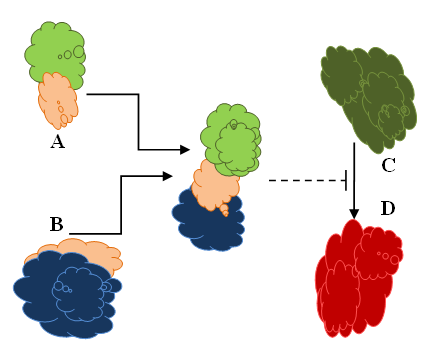
\includegraphics[scale=.45]{diagrams/ProtienProtien.PNG}
		\rule{35em}{0.5pt}
	\caption{A ‘cartoon’ model of protein protein interaction. Two different molecular species A and B bind to
		 form a complex molecular. The newly formed complex hinder the rate at which molecules of species 
		 C are transformed to species D.}
	\label{fig:Protein protein interaction}
\end{figure}

A major drawback of these cartoon models is that while considering system behaviour they could be significantly 
ambiguous. It even more, if there is any interaction network related with feedback. Complexity increases even
further when the number of components and their corresponding interactions in the network grows. Sometimes it
become very difficult to get the intuitive understanding of the system behaviour. But a mathematical model or
description of the same model can eliminate uncertainty of the model behaviour. The mathematical model will 
consider the quantitative representation of individual interaction of the cartoon model. 
In Figure \ref{fig:Protein protein interaction} species A and B bind to form a new complex. 
The newly formed complex hinder the rate at which molecules of species C are transformed to species D.
A numerical description of the process is required to quantify the interaction. 
Though for simple cases only equilibrium condition is enough, but in many other cases binding and 
unbinding rates might be also required. The cartoon model or traditional knowledge cannot provide a quantitative
description rather a qualitative explanation of the molecular interaction. But a well studied mechanisms with
sufficient data might be capable to show the quantitative characteristics. The interaction diagram with
related quantitative data can be used to develop a dynamic mathematical model. This kind of model consists
a number of equations that describe the systems behaviour over time. This behaviour is termed as ``system's dynamic 
behaviour''. These models are usually \textit{mechanistic}, as they explain the mechanisms of molecular interaction
with some laws of physics and chemistry as well as mathematics. Any of the part of the mechanistic model actually
represent the real observed system. Any change in the mechanistic model's component will also mimic to the real
system. So, model simulation (\textit{in silico} experiments) can be used to predict system behaviour. Some numerical
software built with different programming language are used for this simulation purposes. 

As mathematical model is a hypothesis, so the outcome or result of the model hypothesis are also hypothesis.
Though the real cellular behaviour definitively cannot predict by simulation, but they can be invaluable for 
further experimental design by showing the promising paths for further investigation, or by showing the 
inconsistencies between the real laboratory observations and our understanding about the model or system.

\section{The Systeome Project}
"Systeome" is an collection of system profile for all genetic variations and environmental stimuli response. 
A system profile consists of a set of information about the properties of the system
including structure, behaviour, analysis of result such as bifurcation diagram or phase portfolio. The structure
of the system should include structure of gene and metabolic networks and its physical structure, associated constants,
and their properties (\cite{Kitano:2002}).

Systeome is not just a simple cascade map rather it assumes different active and dynamic solutions, simulations as
well as profiling of various system status. The Systeome project might be established with dealing all aspects for
profiling the Systeome of yeast, \textit{C. elegans, Drosophila,} mouse and finally human.
The primary goal of the Human Systeome project is defined as-
``To complete a detailed and comprehensive simulation model of the human cell at an estimated error margin of 
20 percent by the year 2020, and to finish identifying the system profile for all genetic variations, 
drug responses, and environmental stimuli by the year 2030''(\cite{Kitano:2002}).

This is a highly ambitious project, and requires several milestones. Some pilot projects will lead toward the final
goal. Initial pilot projects are using yeast for the simplicity of structure and subsequent behaviour.
\textit{C.elegans} have comparatively complex system structure and so is their behaviour. Beside such pilot projects
concurrently the Human Systeome project shall be commenced.

The futuristic impact of this project will be very wide spread as well as far-reaching. These will be the baseline
and standard asset for any further biological research to provide fundamental diagnostics and prediction for a variety
of medical practice. This Systeome project involves many other major engineering projects for developing the 
measurements, as well as software platform.

\section{\textit{Caenorhabditis elegans}}
\textit{Caenorhabditis elegans} is a nonparasitic, soil dwelling, small nematode worm. \textit{C. elegans} and 
other \textit{Caenorhabditis} species are found through all over the world. It can easily colonize 
mostly in the rotting materials with other microorganism. 
\textit{C. elegans} is easy to maintain in the petri dishes at the laboratory. At $25\,^{\circ}{\rm C}$
\textit{C. elegans} completeits life cycle in just 2.5 days from fertilized embryos to egg-laying 
adult through 4 larval stages. Its typical life span is 2-3 weeks. In 1965, Sydney Brenner 
introduced \textit{Caenorhabditis elegans} as a model organism to study the behaviour and development 
of animal (\cite{Brenner:1974}).

\textit{C. elegans} is a relatively new addition as a model organism but its biological characteristics 
and property already been studied to an extraordinary level. The anatomical characteristics and 
detail development of this nematode was facilitated by its simple body plan. Its an eukaryote and
it shares cellular and molecular structures and control pathways with higher organism. \textit{C. elegans}
is multicellular, an adult wild type  consist of 959 somatic cells and among these 302 are neurons
(\cite{Sulston:1977, Palikaras:2013}). Its developmental process like embryogenesis, morphogenesis 
goes through a complex process to growth to an adult. Yet monitoring of the cellular process 
and recording of cell division pattern is comparatively easier as its body is transparent. 
C Elegan's complete cell lineage at the electron microscopy level has been completed. 
Its already been established and this cell lineage is remarkably invariant between animal to
animal (\cite{Brenner:1974, Byerly:1976, Sulston:1980, Wood:1988}).

\begin{figure}[htbp]
	\centering
		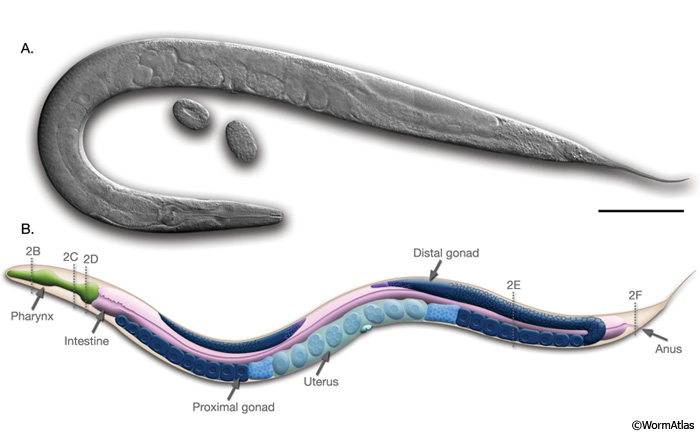
\includegraphics[width=8cm,keepaspectratio]{diagrams/introfig1lr.jpg}
		%\includegraphics[width=10cm,height=3cm,keepaspectratio]{diagrams/introfig5.jpg}
		%\includegraphics{diagrams/Electron.pdf}
		\rule{35em}{0.5pt}
	\caption[Anatomy of an adult]{Anatomy of an adult hermaphrodite(\textit{C.elegans}). 
	A. DIC image of an adult hermaphrodite, left lateral side. Scale bar 0.1 mm. 
	B. Schematic drawing of anatomical structures, left lateral side 
	%(Courtesy of WormAtlas \href{http://www.wormatlas.org/hermaphrodite/introduction/IMAGES/introfig1leg.htm}{here}).}
	(Courtesy of WormAtlas \url{http://www.wormatlas.org/hermaphrodite/introduction/IMAGES/introfig1leg.htm}).}
	\label{fig:anatomy}
\end{figure}

To elucidate pathways and processes relevant to human biology 
and disease C. Elegans is using as a vital model. There are between $\sim20,250$ to $\sim21,700$ 
predicted protein-coding genes in \textit{C. elegans} (\cite{Gerstein:2010}).
Using four different orthology-prediction methods \cite{Daniel:2011} assayed four methods 
to compile a list of \textit{C. elegans} orthologs of human genes. 
A  list of 7,663 unique protein-coding genes were resulted in that list and this
represents $\sim38\%$ of the 20,250 protein-coding genes predicted in \textit{C. elegans}. When human genes 
introduced into \textit{C. elegans} human genes replaced their homologs. On the contrary, many \textit{C. elegans}
genes can function with great deal of similarity to human like mammalian genes. So, 
the biological insight acquire from \textit{C. elegans} may be directly applicable to more 
complex organism like human.

\section{Transcription}

All the process in the body take places through some proteins. So, cells needs protein continuously. 
On the consequences, protein are required to be manufactured at every moment in the body. Inside cell 
protein is manufactured from the DNA. When any cells in the body is in need of protein, a special signal 
is sent to the DNA using hormones. Then proteins reside in DNA start to manufacture based on the 
received codes. The way that the enzymes finds the information required for protein construction is 
extremely complicated.

DNA (Deoxyribonucleic acid) transcription is a process that involves the transcribing of 
genetic information from DNA to a complementary RNA (Ribonucleic acid). Protein is produced 
from the copy of DNA by the transcription process. This production of proteins and enzymes 
are controlled by the coding of cellular activity. Even the conversion of DNA to proteins 
is not straight forward. An RNA polymerase read the sequence of DNA, which produce an 
complementary RNA. DNA consists of four nucleotide bases named adenine (A), guanine (G), 
cytosine (C) and thymine (T) that are paired together (A-T and C-G) to give DNA its double 
helical shape. The major steps to the process of DNA transcription are :


\begin{figure}[tb]
	\centering
		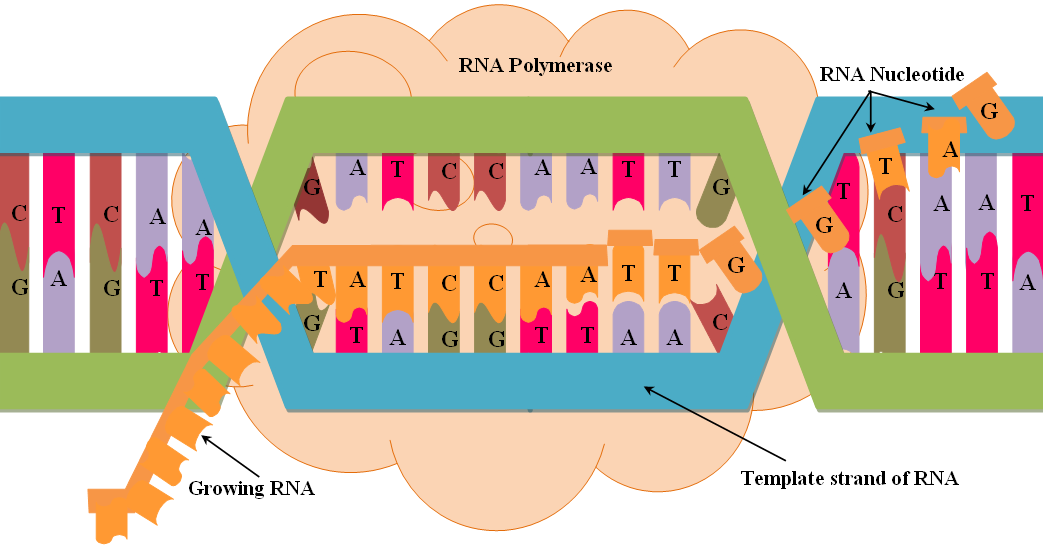
\includegraphics[width=0.7\textwidth,keepaspectratio]{diagrams/Transcription.png}
		%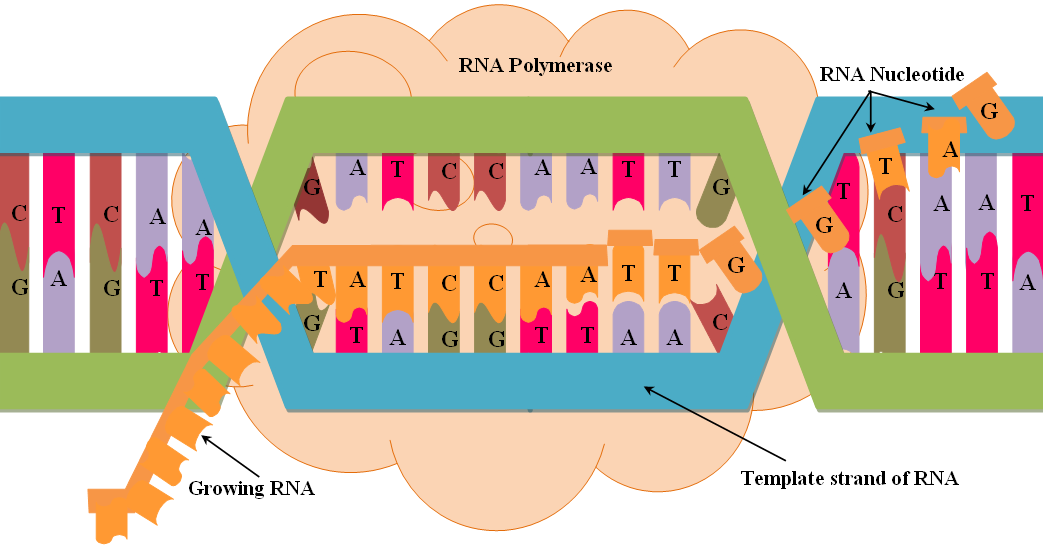
\includegraphics[width=\textwidth,keepaspectratio]{diagrams/Transcription.png}
		\rule{35em}{0.5pt}
	\caption{DNA Transcription}
	\label{fig:transcription}
	%\caption[Anatomy of an adult]{DNA Transcribed in mRNA and mRNA Translated in to Protein
	%(Courtesy of WormAtlas \href{http://www.wormatlas.org/hermaphrodite/introduction/IMAGES/introfig1leg.htm}{here}).}
	%(Courtesy of Perason Education \url{http://www.????.htm}).}
	%\label{fig:DNAtoProtein}
\end{figure}



\begin{figure}[htbp]
	\centering
		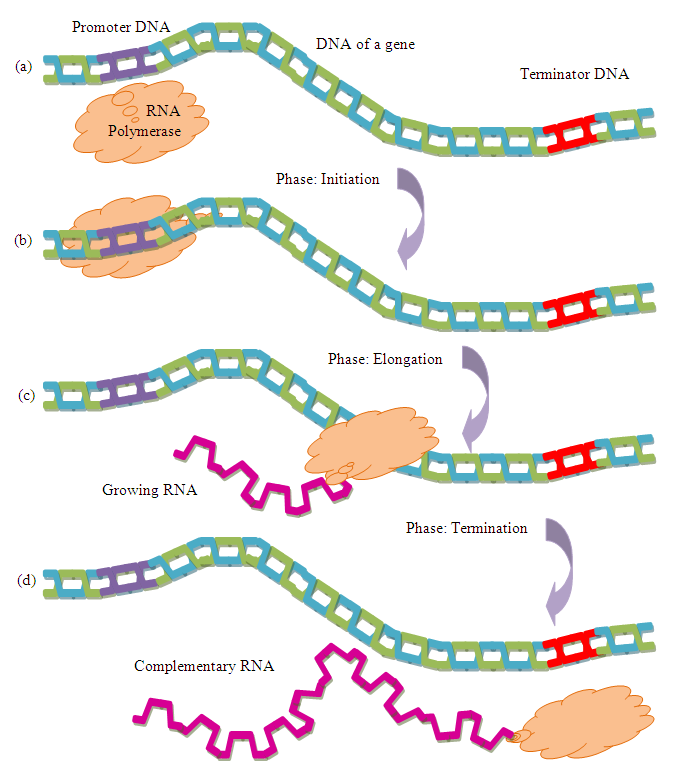
\includegraphics[scale=.6]{diagrams/transcriptionProcess.PNG}
		%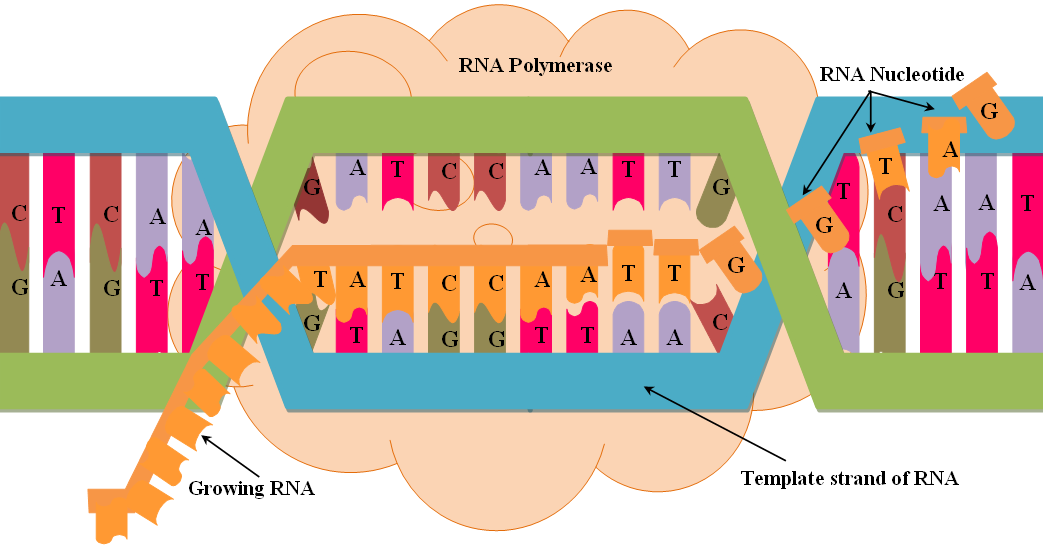
\includegraphics[width=\textwidth,keepaspectratio]{diagrams/Transcription.png}
		\rule{35em}{0.5pt}
	\caption{Transcription Process: DNA Transcribed in mRNA}
	\label{fig:transcriptionProcess}
	%\caption[Anatomy of an adult]{DNA Transcribed in mRNA and mRNA Translated in to Protein
	%(Courtesy of WormAtlas \href{http://www.wormatlas.org/hermaphrodite/introduction/IMAGES/introfig1leg.htm}{here}).}
	%(Courtesy of Perason Education \url{http://www.????.htm}).}
	%\label{fig:DNAtoProtein}
\end{figure}


\textbf{RNA polymerase binds to DNA:} In order to initiate the DNA transcription RNA polymerase and 
sigma factor form a holoenzyme. Transcription process starts at the promoter region of a 
double-stranded DNA. Sigma factor can recognize the DNA and its promoter region. 

\textbf{Elongation:} A sequence specific DNA binding factors called transcription factors then unwind 
the DNA strand. Elongation of the transcript then continues by the RNA polymerase and a 
sequence of chain is opened up. A messenger RNA (mRNA) is formed when RNA polymerase transcribe 
into a single stranded RNA polymer from a single strand of DNA.

\textbf{Termination:} RNA polymerase moves along the DNA unwinding its double helical form until it 
reaches the terminator sequence. At that point, RNA polymerase detaches from the DNA and 
releases the mRNA polymer. In this way DNA double helix is opened, transcribed and reclosed 
with minimum stress on the DNA molecule. At any certain time many RNA polymerase can transcribe 
a single DNA sequence, which can manufacture a large quantity of protein at once. 

\begin{figure}[]
	\centering
		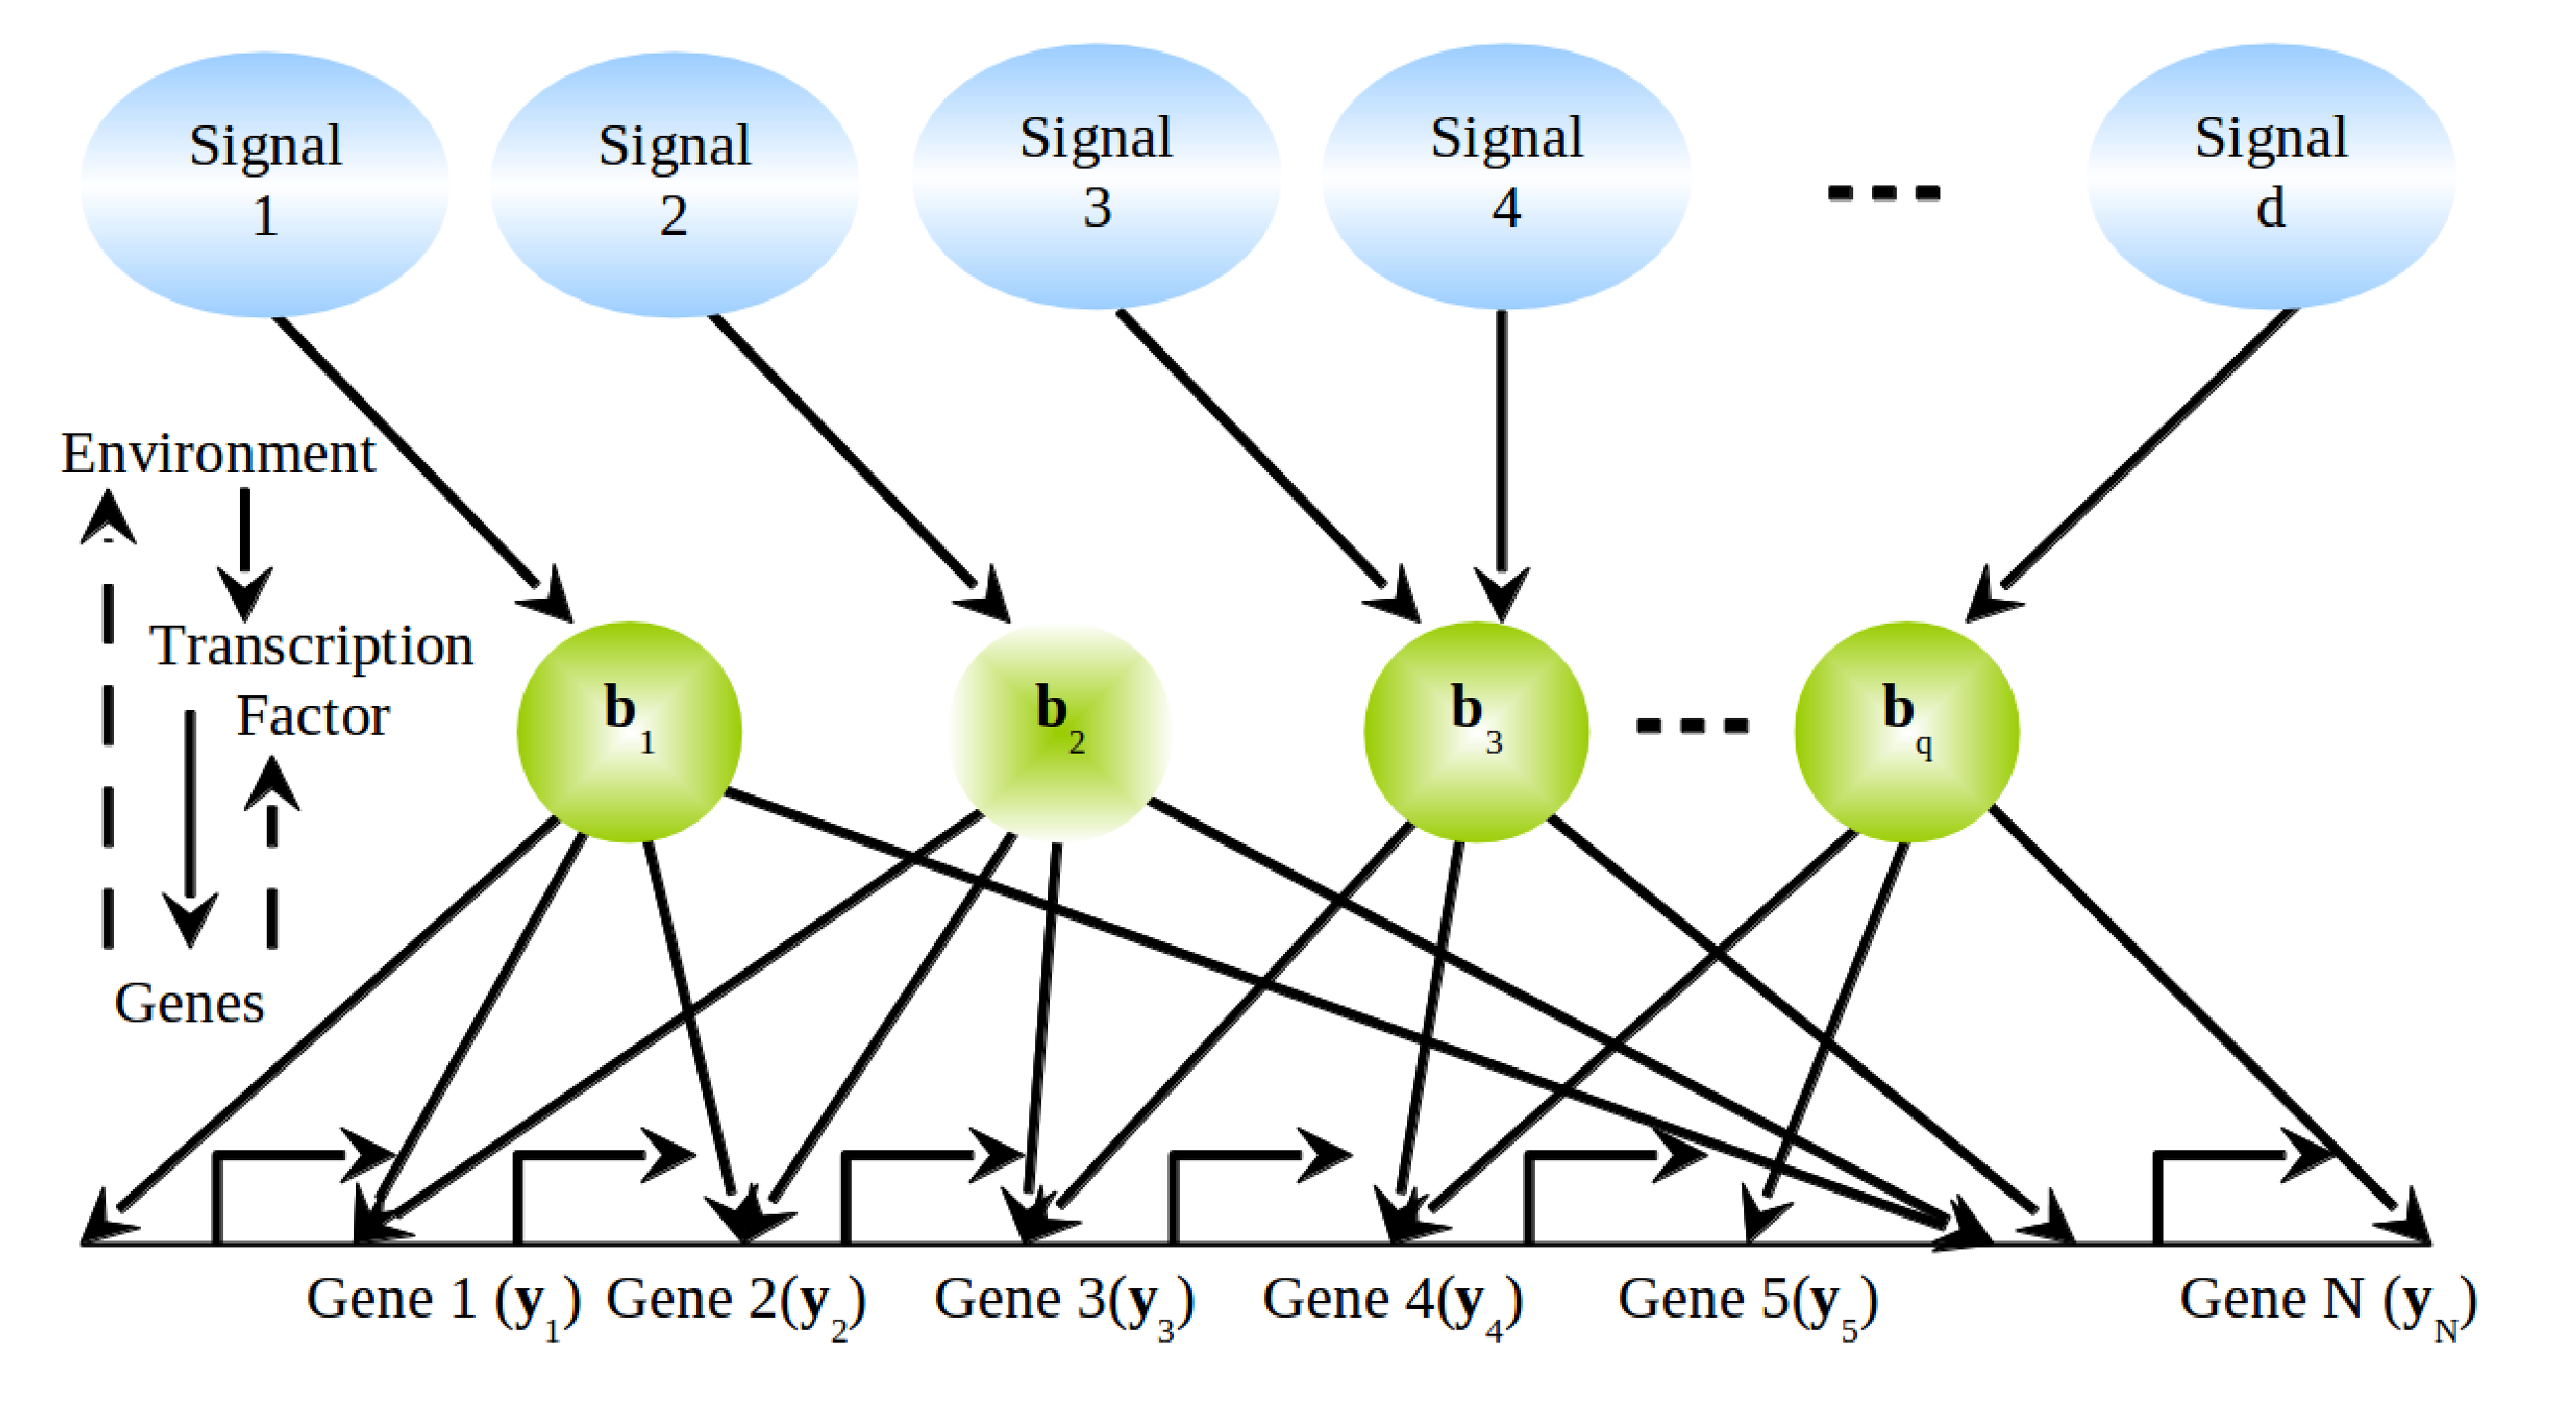
\includegraphics[width=\textwidth,keepaspectratio]{diagrams/MappingEnvironmentalSignal.eps}
		\rule{35em}{0.5pt}
	\caption[The mapping between environmental signal, transcription factor 
	inside the cell the genes that they regulate]{The mapping between environmental signal, transcription factor 
	inside the cell the genes that they regulate.}
	\label{fig:MappingEnvironmentalSignal}
\end{figure}

\section{Transcription Factor}
A transcription factor is a protein that binds to DNA sequences and controls the flow of genetic 
information coding from DNA to mRNA (\cite{karin:1990, Latchman:1997}). Transcription 
factors can both promote or block the transcription process and act as an activator 
or repressor respectively (\cite{Lee:2000, Nikolov:1997, Roeder:1996}). 
A transcription factors may contain one or more DNA-binding domains. These binding domains 
attach to specific sequences of DNA adjacent to the genes that they regulate. Though 
some other protein such as coactivators, deacetylases, chromatin remodelers, kinases, histone 
acetylases, and methylases also play crucial roles in gene regulation but due to lack 
of DNA-binding domains they are not classified as transcription factors 
(\cite{Mitchell:1989, Ptashne:1997, Brivanlou:2002}). 
Figure \ref{fig:MappingEnvironmentalSignal} describes the mapping (we can also say ``cartoon'' mapping) 
between the environmental signal, transcription factors 
inside the cell, and the gene that they regulate. The environmental signal activates 
specific transcription factor proteins. After the activation the transcription factors 
bind DNA to change the transcription rate (the rate at which mRNA is produced) of 
specific target genes. The mRNA is then translated into protein by the process named translation
(\cite{Alon:2006}). 

\section{Key Research Questions}

Key Research questions:
\begin{itemize} 
\item Can we develop a robust data driven dynamic system for gene specific transcription factor 
 activities using Gaussian process over a mechanistic model?
\item Can we step forward to find out the transcription factor activities from a unicellular 
microorganism to multicellular eukaryote?
\item Is it possible to build some replicate specific robust clusters of the gene expression data for \textit{C. elegans}?
\end{itemize} 

%\subsection{A (not so short) Introduction to \LaTeX{}}

%----------------------------------------------------------------------------------------

% Chapter 2

\chapter{Dynamic Modelling of TFAs} % Main chapter title

\label{Chapter2} % For referencing the chapter elsewhere, use \ref{Chapter3} 

\lhead{Chapter 2. \emph{Dynamic Modelling of TFAs}} % This is for the header on each page - perhaps a shortened title

%----------------------------------------------------------------------------------------

% \section{Literature Review}

In modern molecular biology the biological systems like cells are treated as a complex systems.
The usual conception of the complex system is a very large number of simple but identical elements 
interact to generate the complex behaviour. But the actual behaviour of biological systems are 
different from this conception. A vast number of functionally different and multifunctional 
group of elements act with each other selectively, perhaps nonlinearly to generate coherent 
instead of complex behaviour. Mostly, functions of biological systems depend on a combination of 
the network and specific elements involved. 

Development of molecular biology has discovered a large number of biological facts like sequencing 
genome, protein properties etc. But to explain the biological systems behaviour only these are not sufficient.
Study of cell tissues, organs, organisms etc. are also the systems of components to consider and 
their specific interaction which is defined by the evolution could be more supportive to reach the 
prime goal of biology. Though advancement in more accurate quantitative experimental approach will 
continue, but the detail functional insights of biological systems may not give the exact results 
from purely intuitive basis due to the intrinsic complexity of biological systems. A proper 
combination of experimental and computational approaches is more likely to solve this problem.

In modern molecular biology the organisational and functional activity of gene regulatory network 
is a key experimental and computational challenge.

\section{Gene Expression Data for Genomics }
Living cells contains thousands of genes. These genes codes for one or more protein. Expression of 
these genes are regulated by many of these protein through a very complex regulatory pathway.
Usually this regulation occurred to accommodate the change of the environment, as well as through 
the cell cycle of the development process. %TODO
Gene expression is the process where information contains in the gene is used to synthesis a 
functional gene product. The genetic code stored in the DNA usually expressed or interpreted by 
gene expression which represents the  phenotype. 
These gene expression data are usually stored in DNA microarray or DNA chip which is also known as
biochip. 

\begin{figure}[b]
	\centering
		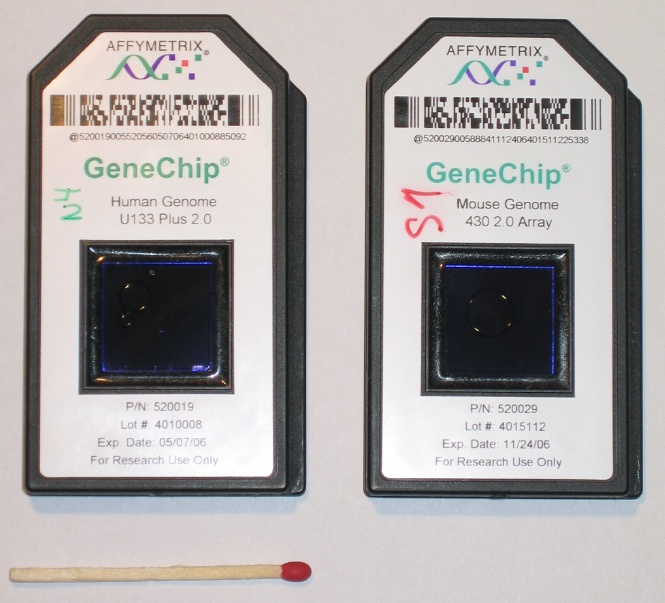
\includegraphics[width=.4\textwidth,keepaspectratio]{diagrams/Affymetrix-microarray.jpg}
		\rule{35em}{0.5pt}
	\caption{Gene Expression Data: Affymetrix Micro Array
	(Image courtesy Wikipedia. 
	\url{http://en.wikipedia.org/wiki/DNA_microarray})}
	\label{fig:Affymetrix-microarray}
\end{figure}
 
Figure \ref{fig:Affymetrix-microarray} shows two Affymetrix chips which contains DNA microarray. 
A match is shown at the bottom for the purpose of size reference of a microarray.
The solid-phase DNA macroarray is usually a collection of ordered microscopic spots called features.
Figure \ref{fig:Gene Expression Microarray} shows the schematic of the gene expression microarray data. 
On a typical Affymetrix microarray there are 6.5 million locations (represented by columns) with 
millions of identical DNA strands in every locations. Every strand construct with 25 probes or bases. 
The microarray is rinsed and washed with fluorescent stain. To accomplish a DNA test, two types of
samples are used one is controlled sample and another is test sample. 
After extracting mRNA from DNA, copied are made from mRNA by reverse transcription. 
Two different fluorescent tagged with cyanide are usually used to differentiate between controlled 
samples and test samples. In general, green is used for controlled copy and red for test copy. 
Then the tagged samples are washed on the microarray. 
DNA is analysed based on matching with the probes on the microarray.
A laser is used to glow the fluorescent molecules. After the hybridisation process
a green spot represents a hybridisation with the controlled targets only, a red spot indicates 
hybridisation with the test targets only, yellow represent hybridisation both with the controlled 
targets and test targets, and black represents hybridisation with the neither samples, i.e. 
no hybridisation. Over the last couple of decades these gene expression data became one of the key 
resource of the biologists to diagnose diseases and drug discovery, gene discovery and determining 
genetic variations, aligning and comparing genetic codes, biomerker development, forensic application, 
functional analysis and also in the field of computational biology.

\cite{Ong:2002} modelled the regulatory pathway in E.coli
from the time series gene expression microarray data by modelling causality, feedback loops or 
hidden variables using a Dynamic Bayesian network and tried to gain the insight of regulatory pathway.
By analysing gene expression data \cite{Friedman:2000} were the first to determine the properties 
of transcriptional program for Baker's yeast using a Bayesian network.

\begin{figure}[t]
	\centering
		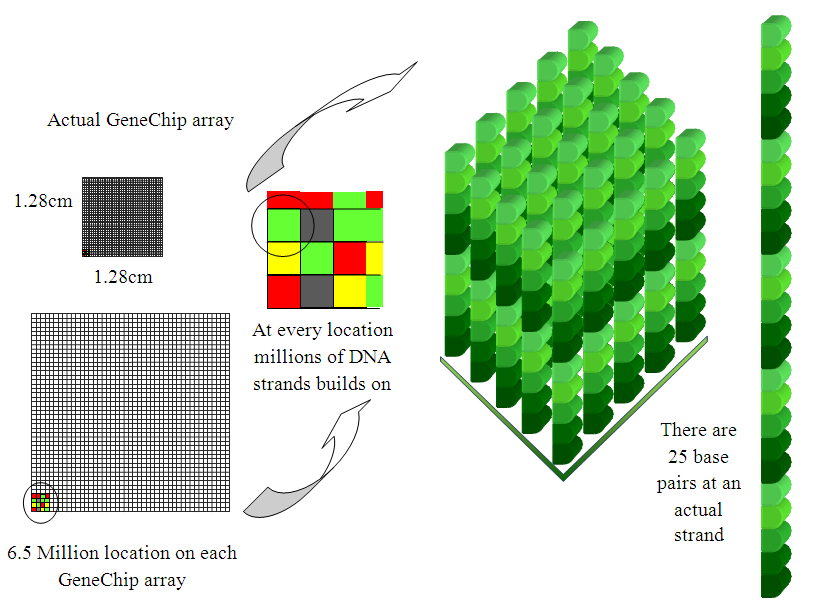
\includegraphics[width=\textwidth,keepaspectratio]{diagrams/GeneExpressionMicroarray.PNG}
		\rule{35em}{0.5pt}
	\caption{Gene Expression Data: Affymetrix Micro Array}
	\label{fig:Gene Expression Microarray}
\end{figure}

Many of the recent studies already established 
the fact that the gene function of regulatory network depends on qualitative as well as 
quantitative aspects of the organisation of the network like high throughput data, including 
genomic sequence, expression profiles and transcription factor.

Among them one of the major challenges is to quantitative measurement and analysis of the 
mechanisms regulating mRNA transcription. Though using high throughput techniques it is 
comparatively easier to measure the output of transcription, but it is experimentally 
very complicated to measure the protein concentration levels of transcription factors and 
chemical affinity to the genes. Very often transcription factors are post-transcriptionally modified. 
So, the actual protein concentration levels and binding affinities could be an unreliable proxy 
of the mRNA expression levels of transcription factors (\cite{Sanguinetti:2006}).

Due to the advancement of the experimental technique lot of interest in recent years has been 
growing to infer information about regulatory activity from target genes. Now biologists can 
acquire the information about the structure of the transcriptional regulatory network.  
\cite{Lee:2002} determined the transcriptional regulatory network of yeast using 
chromatin immunoprecipitation(ChIP). They tried to figure out how yeast transcriptional regulators 
bind to promoter sequences across the genome. By calculating a confidence value (\textit{P} value)
and setting up specific threshold they considered the protein-DNA interactions and artificially
imposes a binding or not binding binary decision for each of the protein- DNA pair.

\section{Connectivity Information}
\cite{Xie:2005} used motif conservation information for higher organisms like human, dog, rat 
and mouse. For promoter analysis they considered a number of network motif 
(also known as transcription factor binding sites) and also some new motifs. These type of data termed as 
connectivity data \cite{Liao:2003} provide information about whether a certain transcription factor 
can bind the promoter region of a gene or not.

\section{Different models of TFAs}
In recent years most methods aim to infer a matrix of transcription factor activities (TFAs).
These TFAs are sum up in a single number at a certain experimental point to find 
the concentration of the transcription factor and its binding affinity to its target genes. 
Many of the researcher used different ways or algorithm to find out these TFAs. 
For example, \cite{Liao:2003} developed a data decomposition technique with dimension reduction and 
introduced ‘network component analysis’. This method takes account of the connectivity information 
by imposing algebraic constraints on the factors. They argued that classical statistical methods
such as principal component analysis and independent component analysis dose not consider the underlying 
network structure while computing low dimensional or hidden representation of a high-dimensional data sets 
like DNA microarray. 

\cite{Alter:2004} used a dimension reduction technique (SVD) to figure out TFAs and also the 
correlation between DNA replication initiation and RNA transcription during the yeast cell cycle. 
Using multivariate regression and backward variable selection 
to identify active transcription factors \cite{Gao:2004} targeted the same; 
\cite{Boulesteix:2005} used partial least squares (PLS) regression to infer the true TFAs 
from a combination of tRNA expression and DNA protein binding measurement. 
A major drawback of the above mentioned methods is that transcription factor activities do not 
hold any information regarding the strength of the regulators interactivity between the 
transcription factor and its different target genes. But it is expected that 
depending on the experimental conditions transcription factor activities can vary from gene to gene. 
Even it is also expected that different transcription factors may bind the same gene. 
In most of the cases, realistic information about the intervals may not be true as they were 
not based on fully probabilistic model. Moreover, false positives are always a problem for 
connectivity data, typically a large portion of Chip data suffers form it 
(\cite{Boulesteix:2005}). 
Furthermore, due to the various cellular process or changes in environmental conditions 
the structure of the regulatory network of the cell can change considerably.
Using regression-based methods it is difficult to track these changes. 
\cite{Nachman:2004} build a probabilistic model, using the basic framework of 
dynamic Bayesian networks using discrete random variables for protein concentrations 
and binding affinities. Though the model was more realistic but the computational complexity for 
genome-wide analysis can be expensive.

\section{Our Goal}
We will propose a dynamic model that extends the linear regression model of \cite{Liao:2003} 
and probabilistic model of \cite{Sanguinetti:2006} to model the distribution of each transcription 
factor acting on each gene. We will model the temporal changes in the gene-specific TFAs from 
time-series gene expression data using Gaussian process (a stochastic process whose consciousness comes from 
random values and where the random variables has a normal distribution and it is associated with every single 
point in a range of times or of space; \textit{Chapter 4} contains detail explanation). 
The covariance structure of the transcription factors will be shared among all genes. 
This approach will lead to a manageable parameter space and figure out useful information about the 
correlation of TFAs.

Initially to build our model we will use two datasets: the classical yeast cell cycle dataset of 
\cite{Spellman:1998} and the yeast metabolic cycle dataset of \cite{Tu:2005}. Both of the data 
sets were used to study the above mentioned models. So, these data will be a source of useful comparisons. 
In both cases the connectivity data will be Chip data (\cite{Lee:2002}; \cite{Harbison:2004}). 
Finally we will use the data set of Caenorhabditis elegans (\textit{C. elegans}) to obtain a deeper insight. 
\textit{C. elegans} was used to build the probabilistic functional gene network Network.


%----------------------------------------------------------------------------------------
%\section{{\color{red}TODO} Regulator density and network motif}
%\cite{Lee:2002} page 800 
% Chapter 3

\chapter{Probabilistic Dynamic Modelling} % Main chapter title

\label{Chapter3} % For referencing the chapter elsewhere, use \ref{Chapter} 

\lhead{Chapter 3. \emph{Probabilistic Dynamic Modelling}} % This is for the header on each page - perhaps a shortened title

%----------------------------------------------------------------------------------------

\section{Probabilistic Modelling}
We have developed our $R$ based tools $chipDyno$ based on the probabilistic approach of \cite{Sanguinetti:2006}.
First we will give a brief introduction of that approach then we will present results.

The logged gene expression measurements are collected in a design matrix , 
$\bold{Y} \in \mathbb{R} ^ { \bold{N} \times \bold{d} }$
where $N$ is the number of genes and $d$ the number of experiments. The connectivity measurements are collected 
in a binary matrix
$\bold{X} \in \mathbb{R} ^ {\bold{N} \times \bold{q}}$, 
where $q$ is the number of transcription factors; element $(i, j)$ of $\textbf{X}$ is one 
if transcription factor $j$ can bind gene $i$, zero otherwise.

In \cite{Sanguinetti:2006}, TFAs are obtained by regressing the gene expressions using the 
connectivity information, giving the following linear model- 
\begin{equation} \label{eq:linear_model}
\bold{y_{n}} = \bold{B_{n}} \bold{x_{n}} + \boldsymbol{\epsilon_{n}}
\end{equation}
Here $n = 1, . . . ,N$ indexes the gene, $\bold{y_{n}}=\bold{Y}(n,:)^T $,
$\bold{x_{n}}=\bold{X}(n,:)^T$ and $\boldsymbol{\epsilon_{n}}$ is an error term. 
The matrix $\bold{B_{n}}$ has $d$ rows and $q$ columns, and models the gene specific TFAs.

As different TFAs for every individual gene will increase number of model parameters drastically. But through
marginalization by prior distribution on the rows of $\bold{B}_n$ these parameters can be dealt. Two plausible 
assumptions for selecting the prior distribution will be helpful to determine the gene specific TFAs.
Firstly, $\bold{b}_{nt}$ has the Markov property and hence gene specific TFA $\bold{b}_{nt} $ at time $t$ depends 
solely on the gene specific TFA at time $(t-1)$ and the second assumption is, the prior distribution to be 
stationary in time.

To satisfy these conditions then there will be two limiting conditions of prior distributions-
Assume all the $\bold{b}_{nt}$ are identical, then the first limiting case will take place. So that
\begin{equation} \label{eq:limit_one_a}
   \bold{b}_{n1} \sim \mathcal{N} ( \boldsymbol{\mu},\bold{\Sigma}), 
\end{equation}
and
\begin{equation} \label{eq:limit_one_b}
   \bold{b}_{n(t+1)} \sim \mathcal{N} ( \bold{b}_{nt},\bold{0})
\end{equation}
If the experimental dataset comes by replicating a condition then this model will be an appropriate model.The second 
limiting case appears when all the $\bold{ b_{nt}}$ are independent and identically distributed-
\begin{equation} \label{eq:limit_two}
   \bold{b}_{nt}\sim \mathcal{N} ( \boldsymbol{\mu},\bold{\Sigma})
\end{equation}
This is the case when experimental dataset comes from independent samples drawn without any temporal order.

\cite{Sanguinetti:2006}  expected a realistic model of time series data to be somewhere in between this two extremes-
\begin{equation} \label{eq:tfa_SanG_update}
  \bold{b}_{n(t+1)} \sim \mathcal{N} (\gamma \bold{b}_{nt} + (1-\gamma)\boldsymbol{\mu},(1-\gamma^2)\bold{\Sigma})
\end{equation}
for $ t= 1, ... , (d-1)$ and $ \bold{b}_{n1} \sim \mathcal{N} ( \boldsymbol{\mu},\bold{\Sigma})$
Where $\gamma$ is a parameter measuring the degree of temporal continuity of the TFAs.
  
If genes are independent for given TFA then the likelihood function is given by:
\begin{equation} \label{eq:likelihood_fnc}
  p\left(\bold{Y|B,X}\right)= \displaystyle \prod_{n \mathop = 1}^{N} p\left(\bold{y}_n|\bold{B}_n,\bold{x}_n\right)
\end{equation}

TFAs can be estimated a posteriori using Bayes’s Theorem-
\begin{equation} \label{eq:Bayes_Theorem}
  p\left(\bold{b}_n|\bold{Y}\right)= \frac {p\left(\bold{Y|b}_n\right) p\left(\bold{b}_n\right)}{p\left(\bold{Y}\right)}
\end{equation}

%----------------------------------------------------------
%----------------------------------------------------------------------------------------
\section{Datasets}
\cite{Sanguinetti:2006} has done their experiments on yeast's cell cycle data of \cite{Spellman:1998} which is a 
unicellular microorganism. One of our research key question was can we step forward to find out the transcription 
factor activities from a unicellular microorganism to multicellular eukaryote. \textit{C. elegans} is a established 
multicellular eukaryotic model organism. To find out the TFA of \textit{C. elegans} basically we had to work with three 
type of datasets. $i).$ Time series data $ii).$ Transcription Factors 
$iii).$ Connectivity information between genes and transcription factors.

\subsection{Time series data}
The gene expression data files came from the Prof. Andrew Cossins's lab, Institute of Integrative Biology, University 
of Liverpool %TODO (Proper reference required!). 
15 Affymetrix single colour GeneChip data on point estimate of expression level came without
estimates of uncertainty level. To extract this data we use the \textit{puma} package (\cite{puma}).
The experimental data had 5 different time points. Apart from the temperature rest of the environmental condition
was same for the consistent result. The experimental data was collected within one day of its
adulthood at the temperature $20\,^{\circ}\mathrm{C}$. To measure the gene response to chill exposure then the
temperature was reduced to $5\,^{\circ}\mathrm{C}$ and experiments were done after one hour, then after 1 day (24 hour), 
then again after 3 days (72 hours) and for final experiments the temperature was set back to $20\,^{\circ}\mathrm{C}$
and data were collected within one day  of rise of temperature. All the experiments were repeated two more times.
i.e. we have 3 independent replicates of similar experiments. Figure \ref{fig:PCA_time_series} shows the PCA 
analysis of the time series data.


\begin{figure}[t]
%\begin{figure}[htbp]
	\centering
		%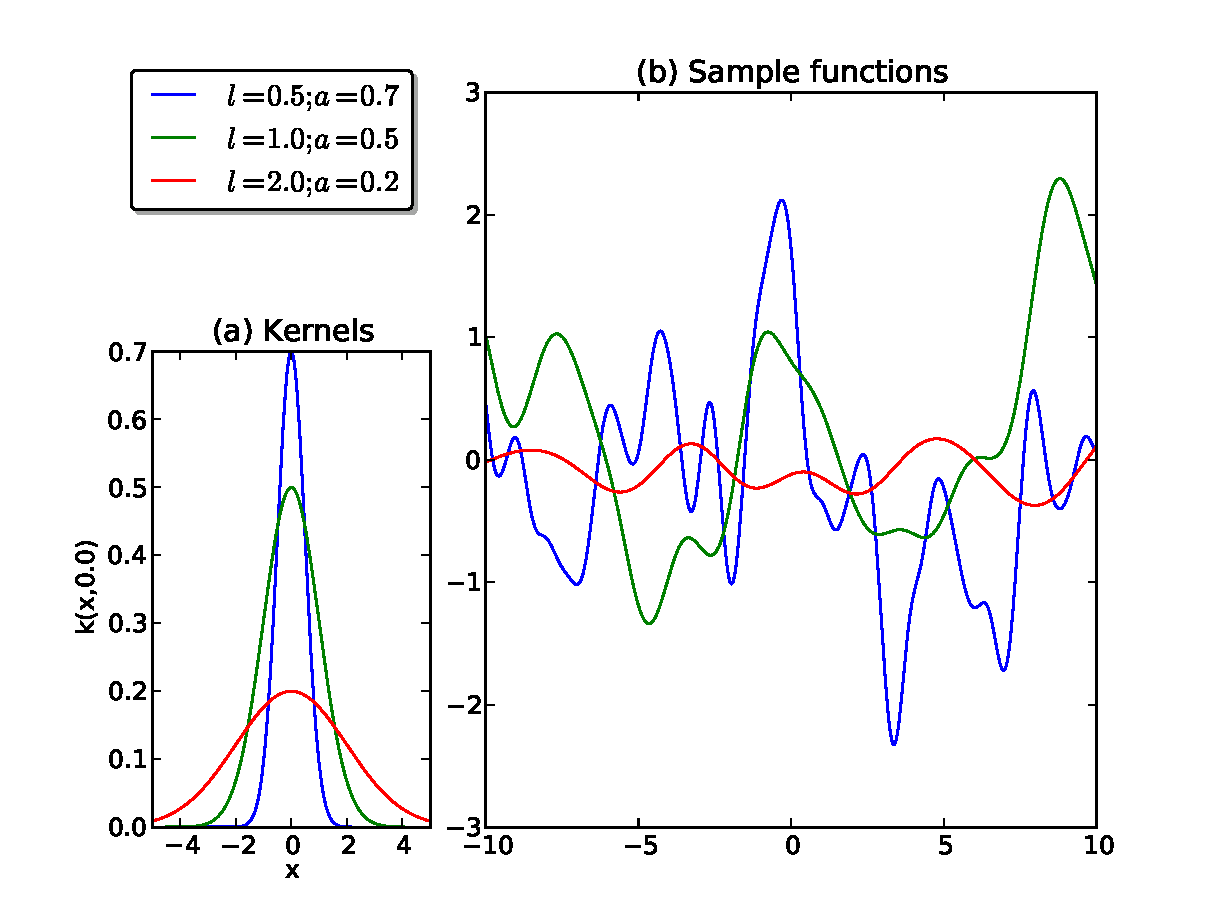
\includegraphics[width=10cm,keepaspectratio]{diagrams/SE_cov.pdf}
		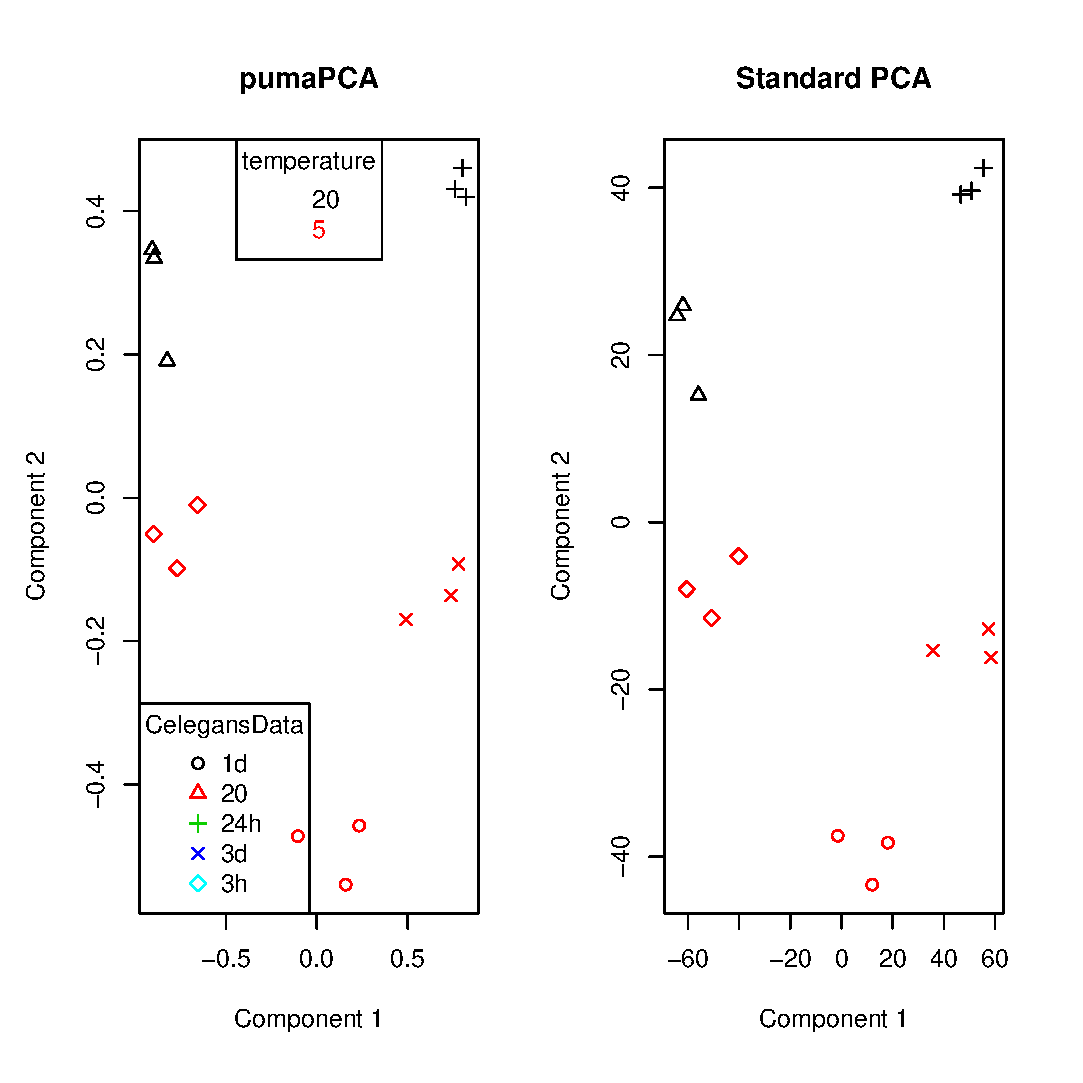
\includegraphics[width=0.7\textwidth,keepaspectratio]{diagrams/PCA2.eps}
		\rule{35em}{0.5pt}
	\caption[Principal component analysis of time series data ]
		{Principal component analysis of gene expression time series data}
	\label{fig:PCA_time_series}
\end{figure}

\subsection{Transcription Factors}
From different data sources we found different number/list of transcription factor. \cite{Inmaculada:2007} 
build a database named \textit{C. elegans} differential gene expression database 
(EDGEdb) which contains the sequence information about 934 predicted transcription factors and
their DNA binding domains. Initially we took these 934 transcription factors for our baseline experimental setup
but we also kept the opening to deal with any number of transcription factor depending on the requirement/ 
update of the sequence information of transcription factors.

\subsection{Connectivity Information}
\cite{WormNet} is a gene network of protein-encoding genes for \textit{C. elegans} based on based on probabilistic function
and modified Bayesian integration. They have considered 15,139 genes and 999,367 linkages between genes 
associated with a log-likelihood score (LLS). These measured scores represents a true functional linkage between a pair 
of genes \cite{Lee:2007}.
The linkage between two genes were measured based on the following evidence codes(\cite{WormNet})-
\begin{itemize}
 \item CE-CC 	Co-citation of worm gene
 \item CE-CX 	Co-expression among worm genes
 \item CE-GN 	Gene neighbourhoods of bacterial and archaeal orthologs of worm genes
 \item CE-GT 	Worm genetic interactions
 \item CE-LC 	Literature curated worm protein physical interactions
 \item CE-PG 	Co-inheritance of bacterial and archaeal orthologs of worm genes
 \item CE-YH 	High-throughput yeast 2-hybrid assays among worm genes
 \item DM-PI 	Fly protein physical interactions
 \item HS-CC 	Co-citation of human genes
 \item HS-CX 	Co-expression among human genes
 \item HS-DC 	Co-occurrence of domains among human proteins
 \item HS-LC 	Literature curated human protein physical interactions
 \item HS-MS 	human protein complexes from affinity purification/mass spectrometry
 \item HS-YH 	High-throughput yeast 2-hybrid assays among human genes
 \item SC-CC 	Co-citation of yeast genes
 \item SC-CX 	Co-expression among yeast genes
 \item SC-DC 	Co-occurrence of domains among yeast proteins
 \item SC-GT 	Yeast genetic interactions
 \item SC-LC 	Literature curated yeast protein physical interactions
 \item SC-MS 	Yeast protein complexes from affinity purification/mass spectrometry
 \item SC-TS 	Yeast protein interactions inferred from tertiary structures of complexes
\end{itemize}

We have constructed the connectivity matrix between genes and associated transcription factors 
from the gene to gene linkage and log-likelihood scores. 
We choose Co-expression among worm genes (CE-CX),
High-throughput yeast 2-hybrid assays among worm genes (CE-YH),
Literature curated human protein physical interactions (HS-LC) and 
High-throughput yeast 2-hybrid assays among human genes (HS-YH) to start our experiments.
But if needed we can consider any of the evidence to reconstruct the connectivity matrix.
From the gene list we have picked the protein-coding genes (i.e. transcription factors) and later 
binarized it. If there is an associated LLS value between a gene and a transcription factor we set the value '1' and 
'0' otherwise.

\section{Result Analysis}
We have developed a $R$ based tool $chipDyno$ for the identification of 
quantitative prediction of regulatory activities of the gene specific TFA through posterior estimation.
The $chipDyno User Guide$ attached at the end of this report explains different functionality 
of this tool and working pathway.

For \textit{C. elegans} gene specific TFA is quite a new experiments. So we didn't find any other result to
consider a baseline and compare our result. 

\begin{figure}[b]
%\begin{figure}[htbp]
	\centering
		%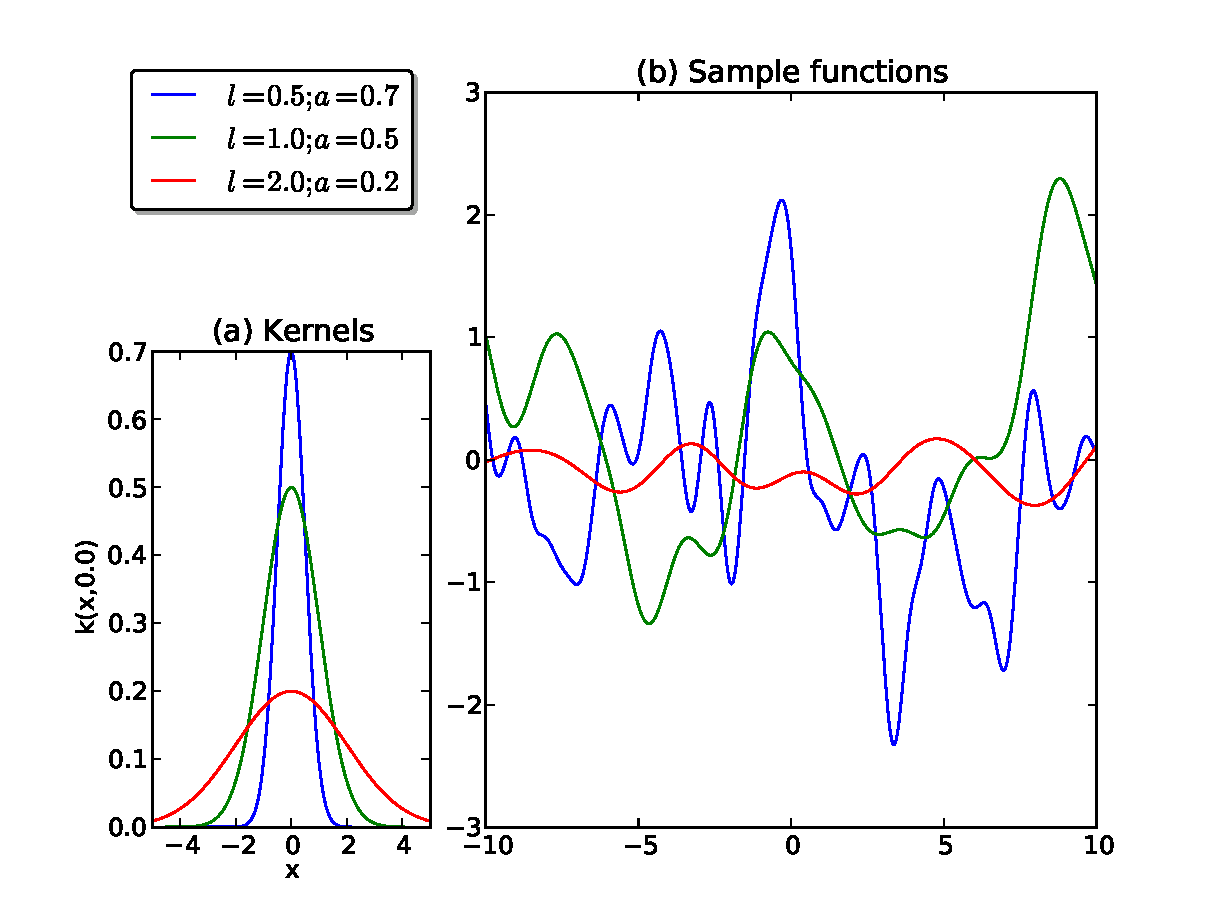
\includegraphics[width=10cm,keepaspectratio]{diagrams/SE_cov.pdf}
		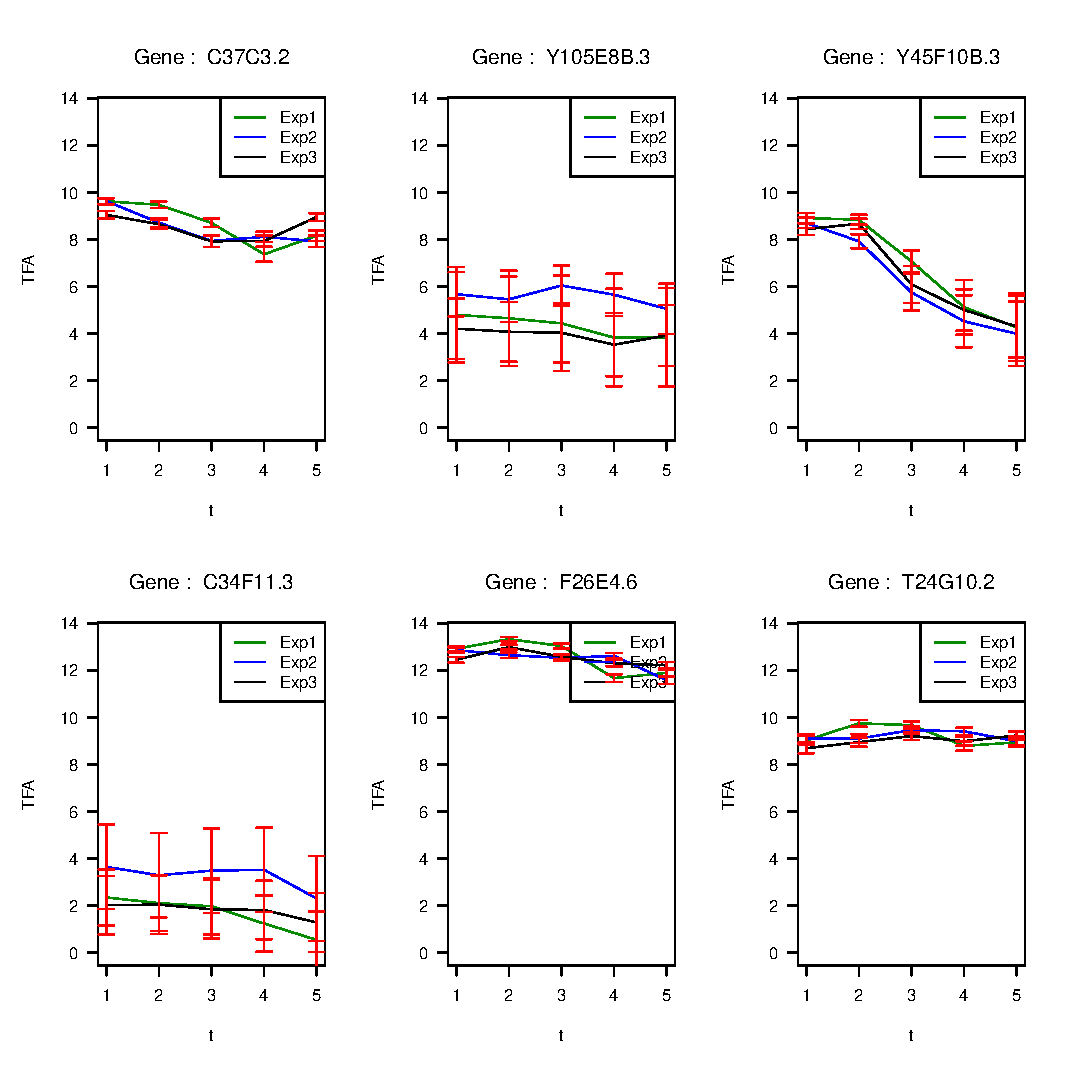
\includegraphics[width=\textwidth,keepaspectratio]{diagrams/ZK370_2_3.eps}
		\rule{35em}{0.5pt}
	\caption[Gene Specific transcription factor activity of ZK370.2]
		{Gene Specific transcription factor activity of ZK370.2}
	\label{fig:TFA_of_of_ZK370.2}
\end{figure}

According to \cite{WormNet} the number of gene of \textit{C. elegans} is 15,139 
and \cite{Inmaculada:2007} presented 934 transcription factors. All the network motif, i.e.
autoregulation, multi-component loop, feedforward loop, single input, multi-input motif, regulator chain
were visible for transcription factor activity. So it was a mammoth task to choose all the transcription
factors and show their activity. Rather we choose some random transcription factor and tried to 
find out its activity on different genes.

\begin{figure}[b]
%\begin{figure}[htbp]
	\centering
		%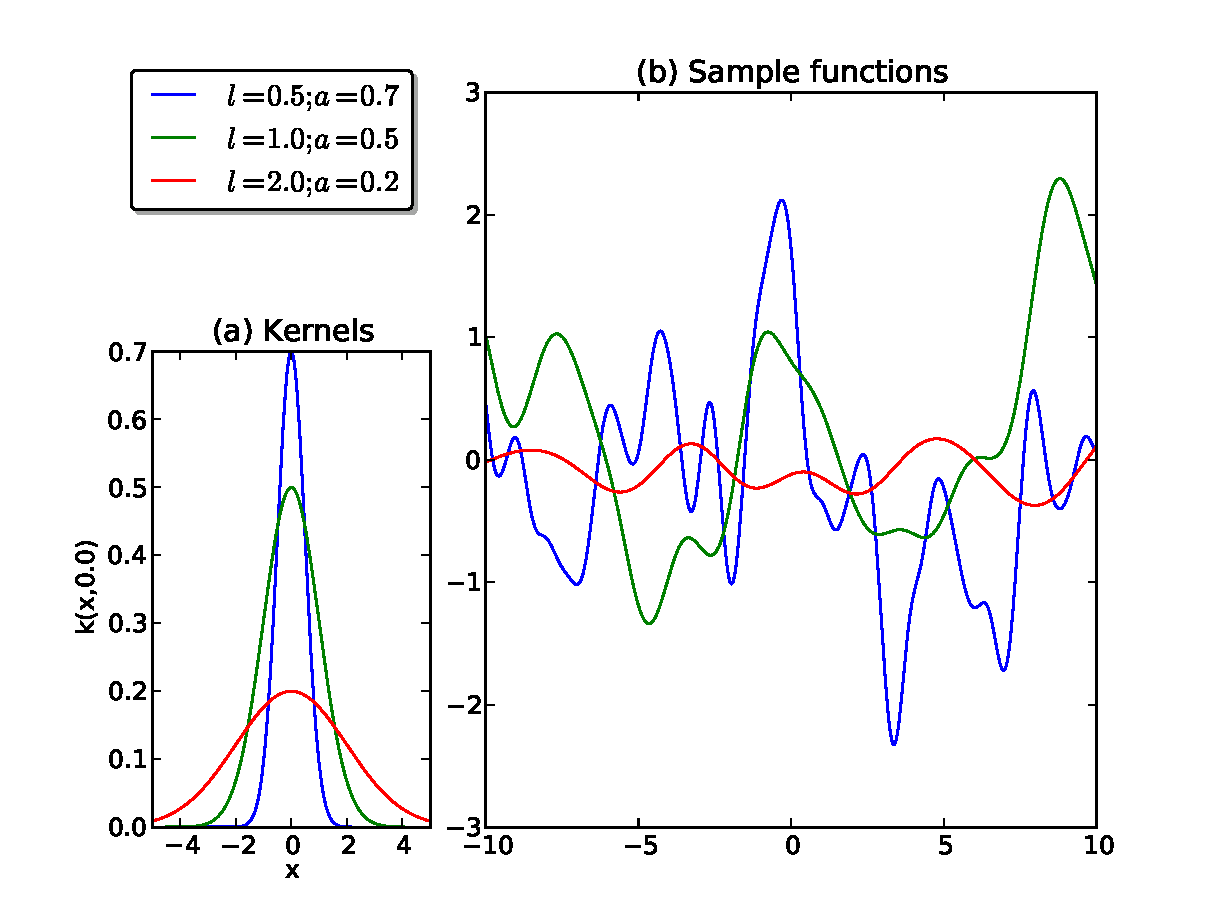
\includegraphics[width=10cm,keepaspectratio]{diagrams/SE_cov.pdf}
		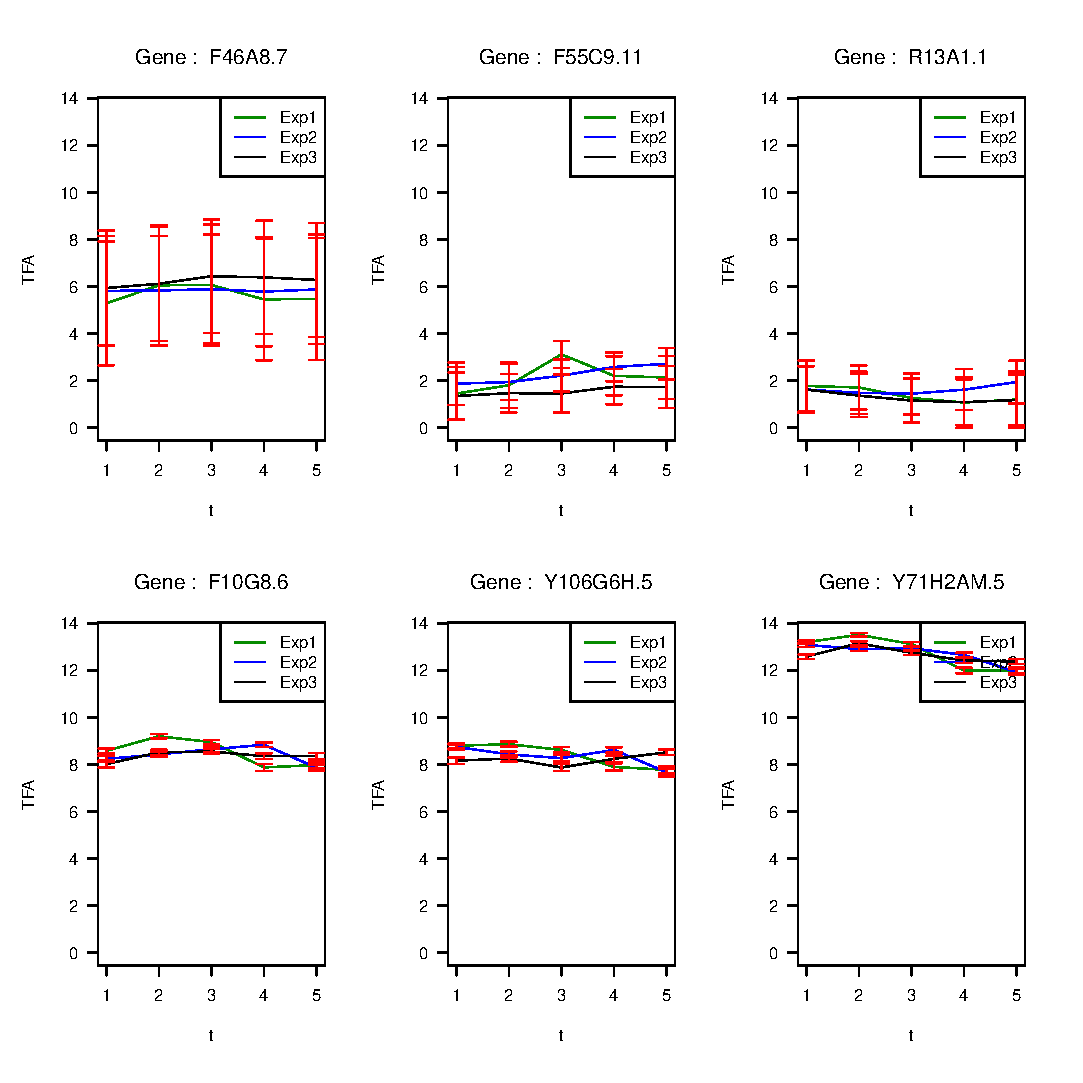
\includegraphics[width=\textwidth,keepaspectratio]{diagrams/T20B12_8_3.eps}
		\rule{35em}{0.5pt}
	\caption[Gene Specific transcription factor activity of T20B12.8.3]
		{Gene Specific transcription factor activity of T20B12.8.3}
	\label{fig:TFA_of_of_T20B12_8_3}
\end{figure}

As a random sample we choose transcription factor ZK370.2 and tried to find its activity on different
genes. Figure \ref{fig:TFA_of_of_ZK370.2} shows that ZK370.2 can act on C37C3.2, Y105E8B.3, Y45F10B.3,
C34F11.3, F26E4.6 and T24G10.2. In the dataset we had three replication of same experimental setup and 
it outcome. We also tried to run our experiments three times and collect the result individually. 
Later we plot all the outcome together.
From the outcome of our experimental result we can say that for some cases (i.e. F26E4.6 and T24G10.2)
the result is very flat and doesn't looks so informative but some of the results represents TFAs varies 
notably over time (i.e. C37C3.2 and Y45F10B.3). 
Perhaps these are the genes which regulates significantly by this transcription
factor. For some cases the error bar is quite high. False positive could be an issue here. The magnitude 
of TFA also differs from one to another.
We picked another random transcription factor T20B12.8.3. Figure \ref{fig:TFA_of_of_T20B12_8_3} shows its
activity on different genes.

\subsection{Gene with multiple regulators}
For the case of multi input motif a single gene could be regulated by multiple transcription factor. Our 
developed tool can determine the posteriori of the relative weight for the different transcription
factors regulating the genes. Table \ref{table:Genes_regulated_by_multiple_TF} shows some examples.
Gene C44B12.5 can be regulated by transcription factor Y116A8C.35 and F33A8.3. While gene
Y105E8B.3 is regulated by T20B12.8, F33A8.3, Y116A8C.35, F11A10.2 and C16A3.7. Though for some cases 
the expression level is quite low and noise margin is significantly high but we can rank these 
gene using \cite{Kalaitzis:2011}.


\begin{table}[htbp!]
	\centering
\begin{tabular}{l l }
      \toprule
      \textbf{Gene Name} & \textbf{Regulators activity} \\
      \midrule
	      {\color{green}C44B12.5} & {\color{blue} Y116A8C.35 }= $ 1.719797 \pm 3.493205 $, \\ 
				    & {\color{blue}F33A8.3} = $ 1.415785 \pm 3.492985$ \\~\\

		{\color{green}Y105E8B.3} & {\color{blue} Y54G2A.1} = $ 0.07157665 \pm 1.2222137 $ \\
		  & {\color{blue} F33D11.12} = $ 0.03861905 \pm 0.7252534 $ \\
 		  & {\color{blue} ZK370.2} = $ -1.20157055 \pm  2.0318513 $\\~\\
		    
	      {\color{green} Y105E8B.3} & {\color{blue} T20B12.8 } = $ 0.25474933 \pm  2.5665869 $ \\
		  			& {\color{blue} F33A8.3 } = $ 0.11619828  \pm  3.5107742 $ \\
 		  			& {\color{blue} Y116A8C.35 } = $ 0.03289664 \pm  3.8071374 $ \\
					& {\color{blue} F11A10.2 } = $ 0.03016348 \pm 1.7737585 $ \\
 		  			& {\color{blue} C16A3.7  } = $ 0.01883489 \pm  $ 0.9431105\\

  \bottomrule
  \end{tabular}
	  \caption[Genes regulated by multiple TF]
		  {Genes regulated by multiple TF}
	  \label{table:Genes_regulated_by_multiple_TF}
\end{table}

\subsection{Different clusters and corresponding active TF}
\cite{Cossins:2007} was also trying to some clusters analysis of the genes based on different
phenotype and its subsequent activities of the cell properties\footnote{The result wasn't published but we came to know 
about it through some discussions.}.
Here are the basic clusters and some of the phenotype properties:

\begin{figure}[]
	\centering
		%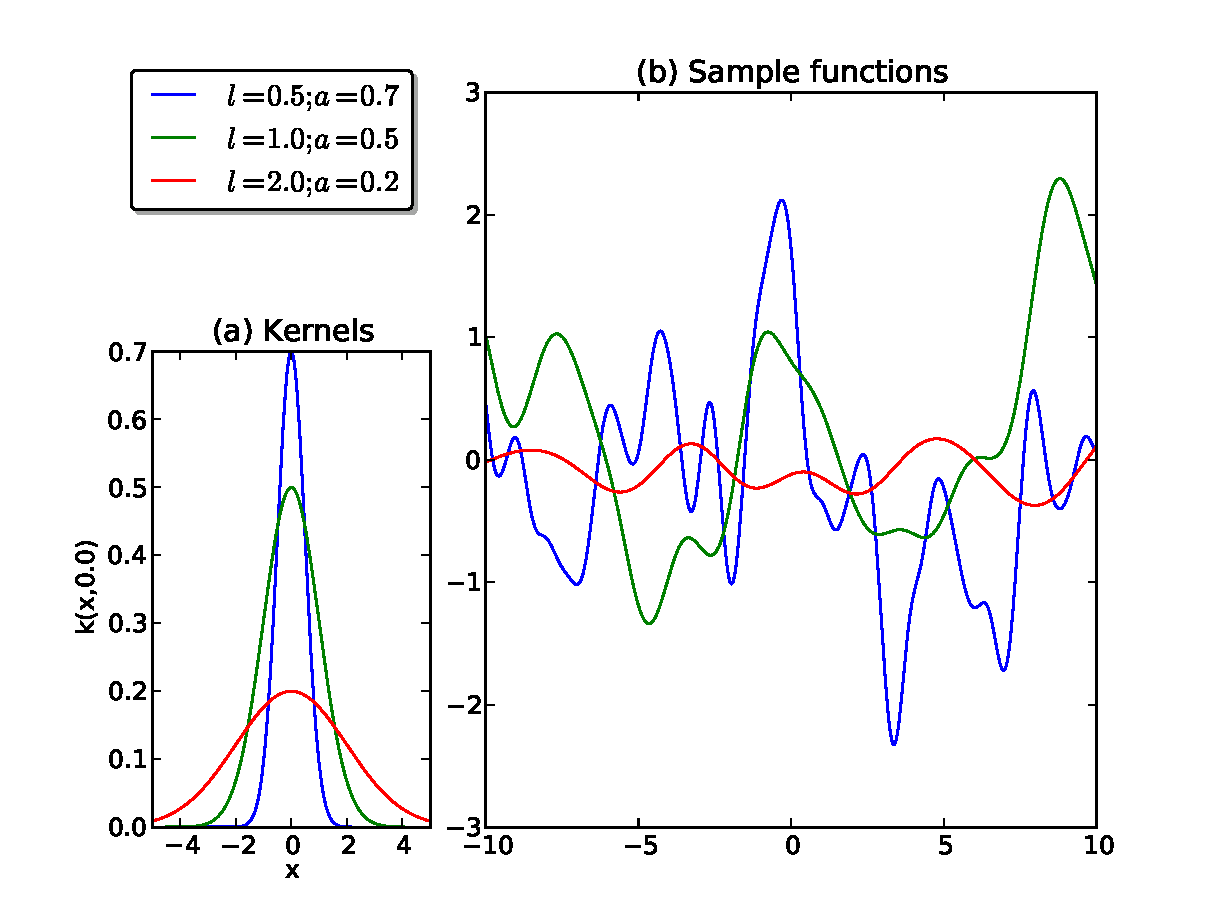
\includegraphics[width=10cm,keepaspectratio]{diagrams/SE_cov.pdf}
		%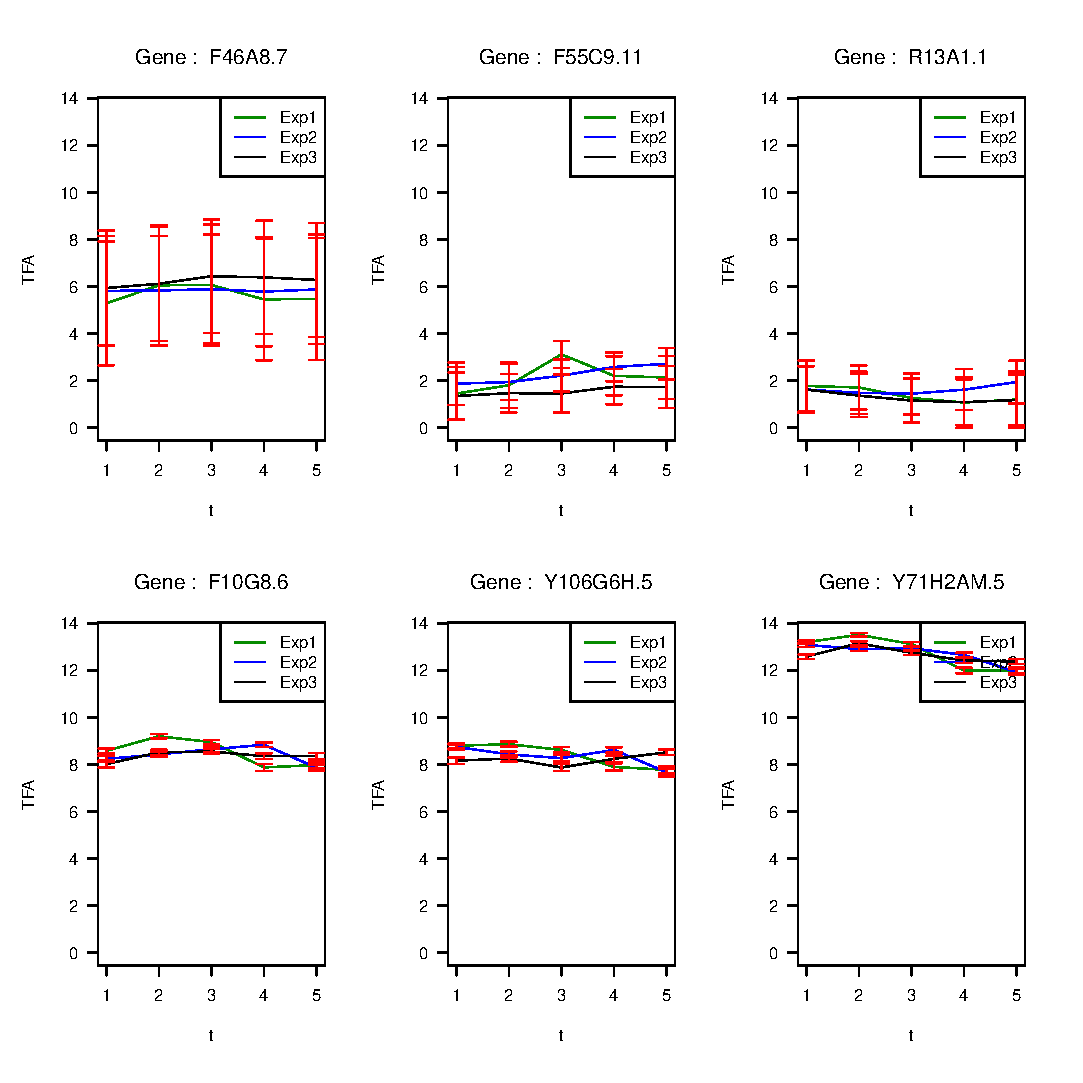
\includegraphics[width=\textwidth,keepaspectratio]{diagrams/T20B12_8_3.eps}
		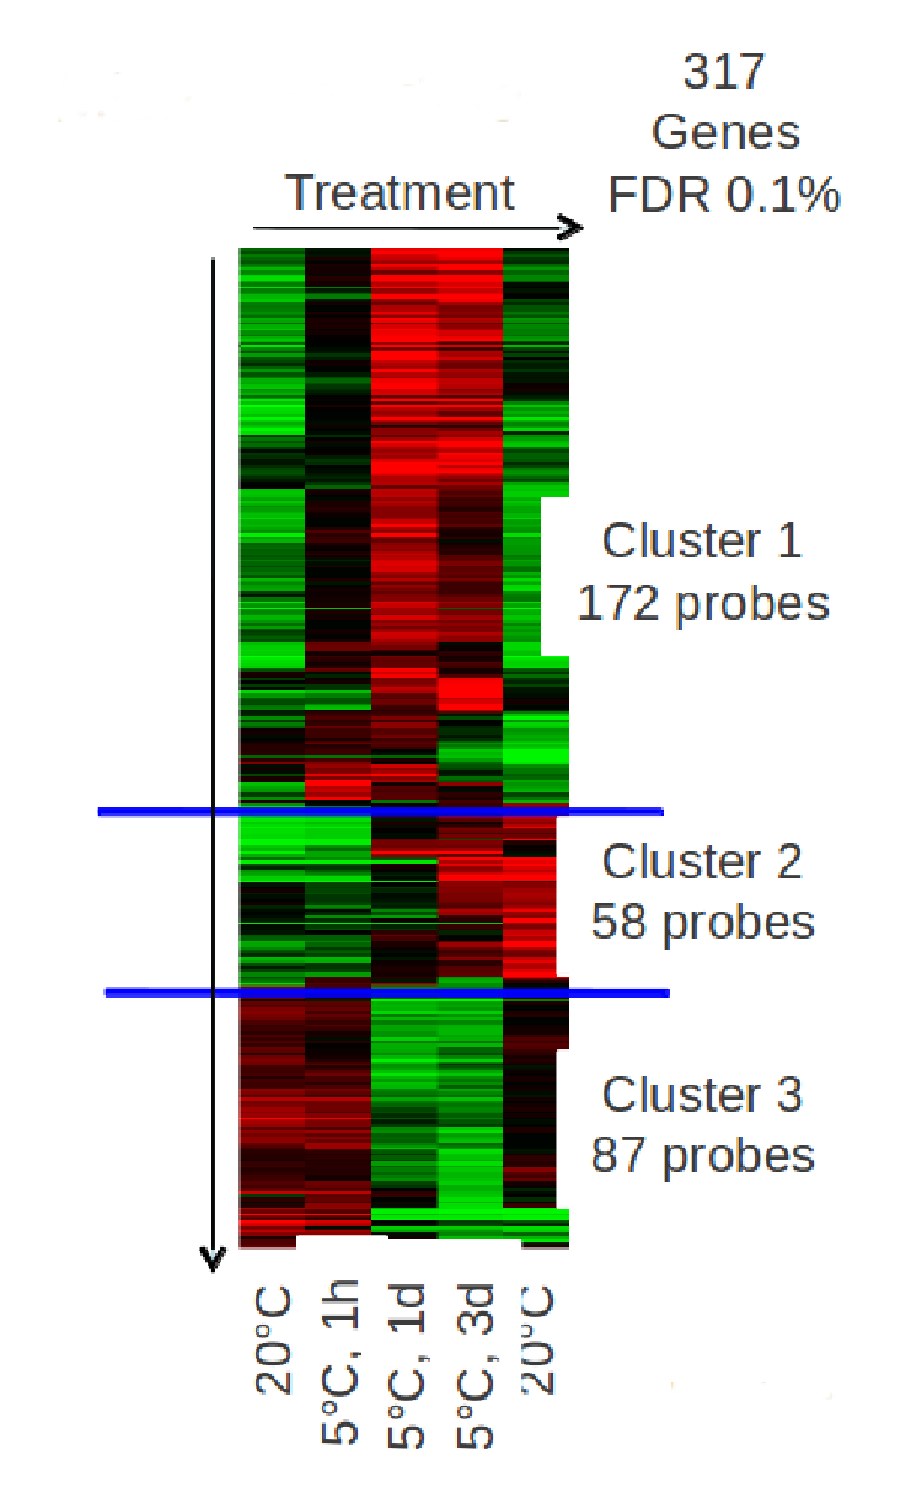
\includegraphics[scale=.5]{diagrams/mcd3.eps}
		\rule{35em}{0.5pt}
	\caption[Clustering of TF]
		{Clustering of TF}
	\label{fig:Clustering_TF}
\end{figure}

\textbf{Cluster 1 - Chill upregulated} basically related with
cell morphogenesis, cell growth, regulation of cell size, electron transport
regulation of cell growth, generation of precursor metabolites and energy,
anatomical structure morphogenesis, cellular metabolic process, proteolysis,
etc.

\textbf{Cluster 2 - Chill late upregulated} related with
chromosome organization and biogenesis, DNA packaging, chromatin architecture
chromatin modification, negative regulation of developmental process, 
chromatin remodelling, regulation of developmental process, DNA metabolic process
larval development (sensu Nematoda), organelle organization and biogenesis, 
post-embryonic development etc.

\textbf{Cluster 3 - Chill downregulated genes} related with
amino acid and derivative metabolic process, carboxylic acid metabolic process,
organic acid metabolic process, fatty acid metabolic process,
amino acid metabolic process, monocarboxylic acid metabolic process, etc. 
Rest of the genes were placed in the group 'Others'.

Figure \ref{fig:Clustering_TF} shows heat map generated from DNA 
microarray data to reflect the gene expression values at
different temperature and their basic clusters \cite{Cossins:2007}\footnote{Some portion of the result
is unpublished result; came to know through a presentation}.
Based on the above clusters we have tried to find out the the transcription factors
active for different clusters. We have managed to find out the active
transcription factor for each clusters and Table \ref{table:Active_TF_diff_clusters}
shows the numbers.


\begin{table}[]
  \centering
  \begin{tabular}{l l }
    \toprule
    \textbf{Clusters} & \textbf{Active TF} \\
    \midrule
    1. {\color{blue}Chill upregulated} & {\color{green}\bf 6} \\ 
    2. {\color{blue}Chill late upregulated} & {\color{green}\bf245} \\ 
    3. {\color{blue}Chill downregulated} & {\color{green}\bf128} \\
    4. {\color{blue} Others} & {\color{green}\bf 203} \\
  \bottomrule
  \end{tabular}
  \caption[Active TF on different clusters]
	  {Active TF on different clusters}
  \label{table:Active_TF_diff_clusters}
\end{table}


\section{Ranking Differentially expressed gene expressions}
\cite{Kalaitzis:2011} analysed the time series gene expression and filter the quiet or inactive genes
from the differentially expressed genes. They have developed the model considering the temporal nature of data 
using Gaussian process. We have used this model to rank our time series gene expression and ranked the 
differentially expressed gene expressions. 
We tried to rank the three replicates of our data separately and later determine the
Pearson correlation between ranking score of different samples.

\begin{figure}[t]
	\centering
		%\includegraphics[scale=.8,keepaspectratio]{diagrams/RankingScoreWithValue.eps}
		\includegraphics[scale=.7,keepaspectratio]{diagrams/RankingScoreLogValue.eps}
		\rule{35em}{0.5pt}
	\caption[Pearson's correlation between different ranking scores]
		{Pearson's correlation between different ranking scores}
	\label{fig:ranking_scores}
\end{figure}

Figure \ref{fig:ranking_scores} shows the Pearson correlation between different ranking scores.
The correlation coefficient for all three relations (between sample 1 and sample 2, sample 2 and sample 3 and
sample 3 and sample 1) were quite high. Which indicates the similarity of 
differentially expressed genes and quiet genes of different samples or replication of time series data.
So, if required, based on these ranking we can easily filter out some of the quiet genes and keep the
other genes for further experiments.
%\section{Pearson correlation between ranked gene expressions}
% Chapter 4

\chapter{Gaussian Process Regression} % Main chapter title

\label{Chapter4} % For referencing the chapter elsewhere, use \ref{Chapter1} 

\lhead{Chapter 4. \emph{Gaussian Process Regression}} % This is for the header on each page - perhaps a shortened title

%----------------------------------------------------------------------------------------

\section{Brief History of Gaussian Process}
The Gaussian processes is one of the most simple and widely used families of stochastic processes 
for modeling dependent data observed over time, or space, or time and space together. As a general
setting, Gaussian process of many types have been studied and incorporated in research for decades.
%L$\acute{e}$vy process
The Wiener process (e.g. \cite{Papoulis:1991}) (one of the best known L\'{e}vy processes) is a 
particular type of Gaussian process. The story of using Gaussian process is still a long one. 
\cite{Kolmogorov:1941} and \cite{Wiener:1949} used Gaussian process for time series prediction
date backs to the 1940's.
But probably the history of Gaussian process is even older. 
The Brownian motion is a Gaussian process. This is because the distribution of a random vector 
is a linear combination of vector which have a normal distribution (\cite{Castaneda:2012}).
Thorvald N. Thiele was the first to propose the mathematical theory of Brownian motion. He also 
introduce the likelihood function during the period 1860-1870 when he was serving 
as a assistant to professor H. L. d'Arrest at the Copenhagen Observatory, Denmark. 

Since the 1970's Gaussian process have been widely adopted in the field of meteorology and
geostatistics. Around that time Gaussian process regression was named as kriging and 
used by \cite{Matheron:1973} for prediction in geostatistics. \cite{O'Hagan:1978} used 
Gaussian process in the field of statistics for multivariate input regression problem.
For general purpose function approximators \cite{Bishop:1995} used neural networks,
\cite{Neal:1996} showed the link between Gaussian process and neural networks and
in the machine learning context \cite{Williams_and_Rasmussen:1996} first described 
Gaussian process regression. 

Over the last two decades Gaussian process in machine learning has turned to a major interest
and much work has been done. \cite{Rasmussen_and_Williams:2006} perhaps the most widely used and 
cited article on Gaussian process for machine learning and most of the discussed in this chapter 
can be found there in detailed form.

%----------------------------------------------------------------------------------------

\section{The Regression Problem}
Machine learning problems can be roughly categorized into three basic classes. 
\begin{enumerate}
 \item Supervised learning: inferring a function from labelled training data
 \item Unsupervised learning: to find hidden structure of unlabelled data 
 \item reinforcement learning: take action by maximizing the cumulative reward. 
\end{enumerate}
\cite{MacKay:2003}, \cite{Bishop:2006} describes the concepts in detail.
Supervised learning may be further sub-categorized in two fundamental tasks: regression and 
classification. Regression problem deals with estimating the relationship among some dependent
variables with some independent variables, whereas classification identifies the desired 
discrete output levels.

Regression is the task of making some prediction of a continuous output variable at a desired
input, based on a training input output data set. The input data can be any type of 
object or real valued features located in $\mathbb{R}^D$ which have some predictability 
for an unobserved location. 

By definition of regression, it is obvious that there will be some inference based on a function
mapping the outputs from a set of given inputs, because by inferring a function we can predict 
the response for a desired input. In the case of Bayesian inference, a prior distribution 
over function is required. Then the model go through some training process and update the prior, 
based on the training data set $\mathcal{D}$ constructed with $N$ input vectors, such as
$\{\textbf{X},\textbf{y}\}$, 
where $\textbf{X}\equiv{\{{\textbf{x}_n}\}_{n=1}^N}$, $ \textbf{x}_n\in\mathbb{R}^D $ 
are the training inputs and 
$\textbf{y}\equiv{\{{y_n}\}_{n=1}^N}$, $ \textbf{y}_i\in\mathbb{R}$
are the training outputs. Now a key question arises, how can we consider a distribution
over an infinite dimensional object as a function?

Although using plain and simple statistics regression
problem can be solved, but to model a more complex and specific learning task with improved
reliability and robustness Gaussian process is a better selection. 
Gaussian process models can be used for regression model having an object featuring 
infinite dimensionality. Even at present Gaussian process have been
advanced beyond the regression model and now using for classification, 
unsupervised learningcite{}, reinforcement learning cite{} and many more. %TODO citation

We assume the outputs considered at the training level may contain some noise and observed
from the underlying mapping function $f(\textbf{x})$. The objective of the regression problem
is to construct $f(\textbf{x})$ from the data $\mathcal{D}$. This task is ill-defined and 
dealing with noisy data leads to an exercise in reasoning under uncertainty. Hence, a single 
estimate of $f(\textbf{x})$ clearly could be misleading, rather a probability distribution over
likely functions could be much more appealing. A regression model based on Gaussian process 
is a fully probabilistic Bayesian model, and definitely will serve for our purpose. In contrast with
other regression models, here we will get the opportunity to choose the best estimate of 
$f(\textbf{x})$. If we consider a probability distribution on functions $p(f)$ as the Bayesian
prior for regression, then from data Bayesian inference can be used to make predictions:
\begin{equation} \label{eq:2.1}
p(f|\mathcal{D})= \frac{p(\mathcal{D}|f)p(f)}{p(\mathcal{D})} 
\end{equation}


The dynamic activity of transcription factors can be viewed as a regression task.

\section{Gaussian Process definition}
A Gaussian process is a collection of random variables, any finite number of which have a 
joint Gaussian distribution (\cite{Rasmussen_and_Williams:2006}). It is a continuous
stochastic process and defines probability distributions for functions. It can be also viewed
as a random variables indexed by a continuous variable: $ f(\textbf{x})$ chosen from a random
function variables $ \textbf{f} = \{ f_1, f_2, f_3,..., f_N\}$, with corresponding indexed inputs
$ \textbf{X} = \{ \textbf{x}_1, \textbf{x}_2, \textbf{x}_3,..., \textbf{x}_N\}$. In Gaussian processes,
variables from these random functions are normally distributed and as a whole can be represent as a
multivariate Gaussian distribution:
\begin{equation} \label{eq:2.2}
p(\textbf{f}|\textbf{X})= \mathcal{N}(\boldsymbol\mu,\textbf{K}),
\end{equation}
where $\boldsymbol\mu$ is the mean and $\textbf{K}$ is covariance of Gaussian distribution
$\mathcal{N}(\boldsymbol\mu,\textbf{K})$
The Gaussian distribution is over vectors but the Gaussian process is over functions.

We need to define the mean function and covariance function for a Gaussian process prior.
If $f(\textbf{x})$ is a real process, a Gaussian process is completely defined by its mean function
and covariance function given in \ref{eq:2.3} and \ref{eq:2.4} respectively.
Usually the $m(\textbf{x})$  and the covariance function $k(\textbf{x},\textbf{x\textprime})$
are defined as-
\begin{equation} \label{eq:2.3}
m(\textbf{x})= \mathbb{E}[f(\textbf{x})],
\end{equation}
\begin{equation} \label{eq:2.4}
k(\textbf{x},\textbf{x\textprime})= 
\mathbb{E}[(f(\textbf{x})-m(\textbf{x}))(f(\textbf{x}\textprime)-m(\textbf{x}\textprime))],
\end{equation}
where $\mathbb{E}$ represents the expected value.
We denote the Gaussian process as-
\begin{equation} \label{eq:GP}
f\left(\textbf{x} \right)\sim \mathcal{GP} \left(m \left(\textbf{x}\right), k \left(\textbf{x},\textbf{x\textprime}\right) \right).
\end{equation}

The covariance matrix $\textbf{K}$ is constructed from the covariance function
$k(\textbf{x},\textbf{x\textprime})$ and 
$\textbf{K}_{ij}=k(\textbf{x}_i,\textbf{x}_j)$.

\section{GP: Covariances}
For convenience, we often define the mean of the prior of the GP as zero but the
posterior mean of the GP $p(f|\mathcal{D})$ obtained from the GP regression is not a zero
mean process.

Based on our problem we are free to design our covariance function. The mandatory requirement 
of a covariance matrix is symmetric positive semi-definite. So as long as the covariance function
generates symmetric positive semi-definite matrix, we can use that function for a Gaussian process.
Smoothness, periodicity, amplitude, lengthscale etc. are the basic properties while choosing 
a Gaussian process covariance function. It is very crucial to choose a appropriate function
for further Gaussian process Modelling. The main goal of this thesis is to develop a
covariance function able to solve our problem, hopefully more robust and flexible way.
Here first we will discuss about some of the very well known and widely used covariance
functions. The in detail description will be found at \cite{Rasmussen_and_Williams:2006}.


\subsection{Exponentiated Quadratic covariance function}
Exponentiated Quadratic covariance is the most widely used covariance function for Gaussian
process. This is also known as squared exponential (SE) covariance or radial basis function (RBF).
The exponentiated quadratic has become the de-facto default kernel for Gaussian process and
has the following form-
\begin{equation} \label{eq:EQ_cov}
K_{EQ}(r)= a^2 \exp \left(-\frac{r^2}{2l^2}\right)
\end{equation}
where $r=\lVert \textbf{x}-\textbf{x}\textprime \rVert$. 
Here $\lVert \textbf{x}-\textbf{x}\textprime \rVert$ is invariant to translation and rotation.
So, Exponentiated Quadratic covariance is stationary, as well as isotropic.
Here the parameter for output variance $a$ and lengthscale parameter $l$ govern the property of
sample functions and commonly known as hyperparameters. Parameter $a$ determines the typical amplitude, i.e. 
average distance of the function away from the mean. $l$ controls the lengthscale, i.e. the length 
of the wiggles of the function. 

\begin{figure}[t]
	\centering
		%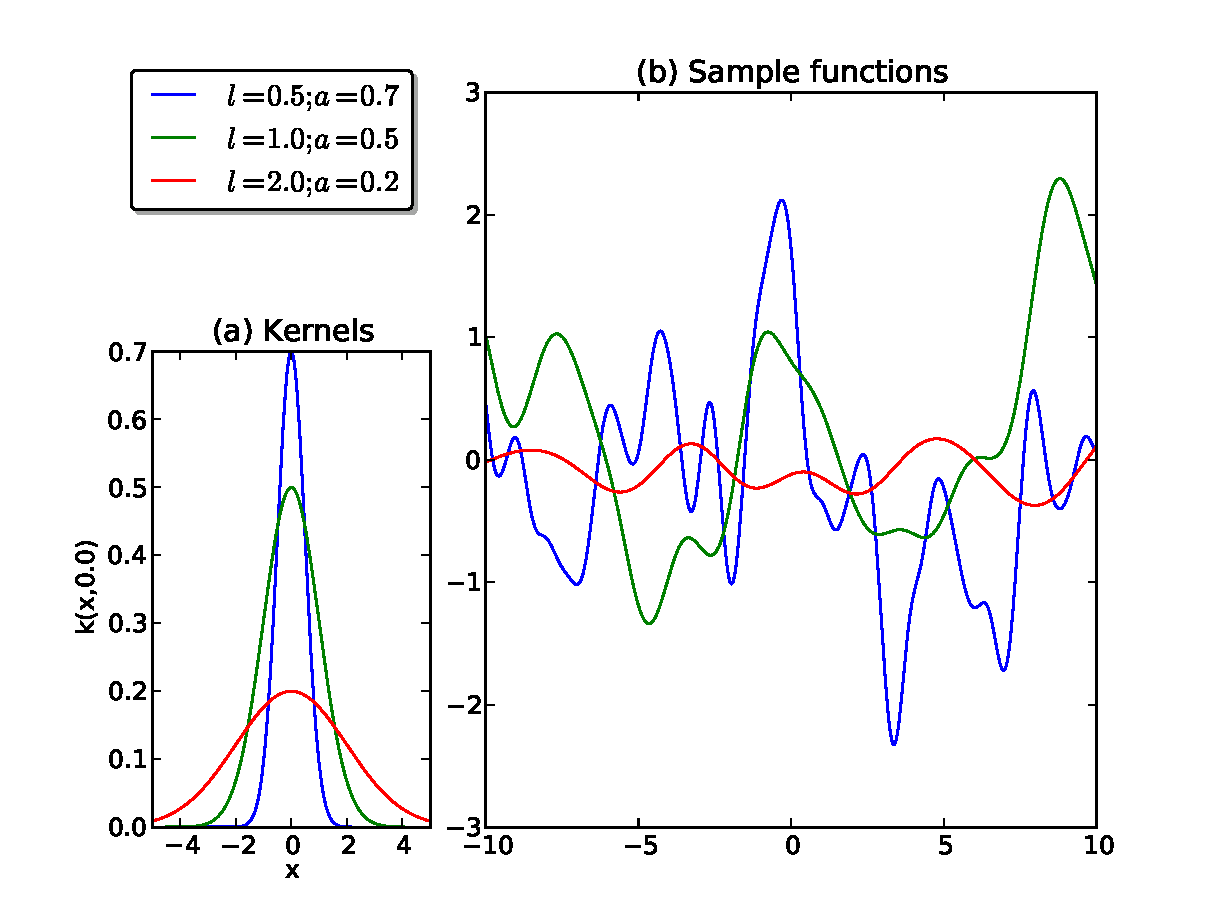
\includegraphics[width=10cm,keepaspectratio]{diagrams/SE_cov.pdf}
		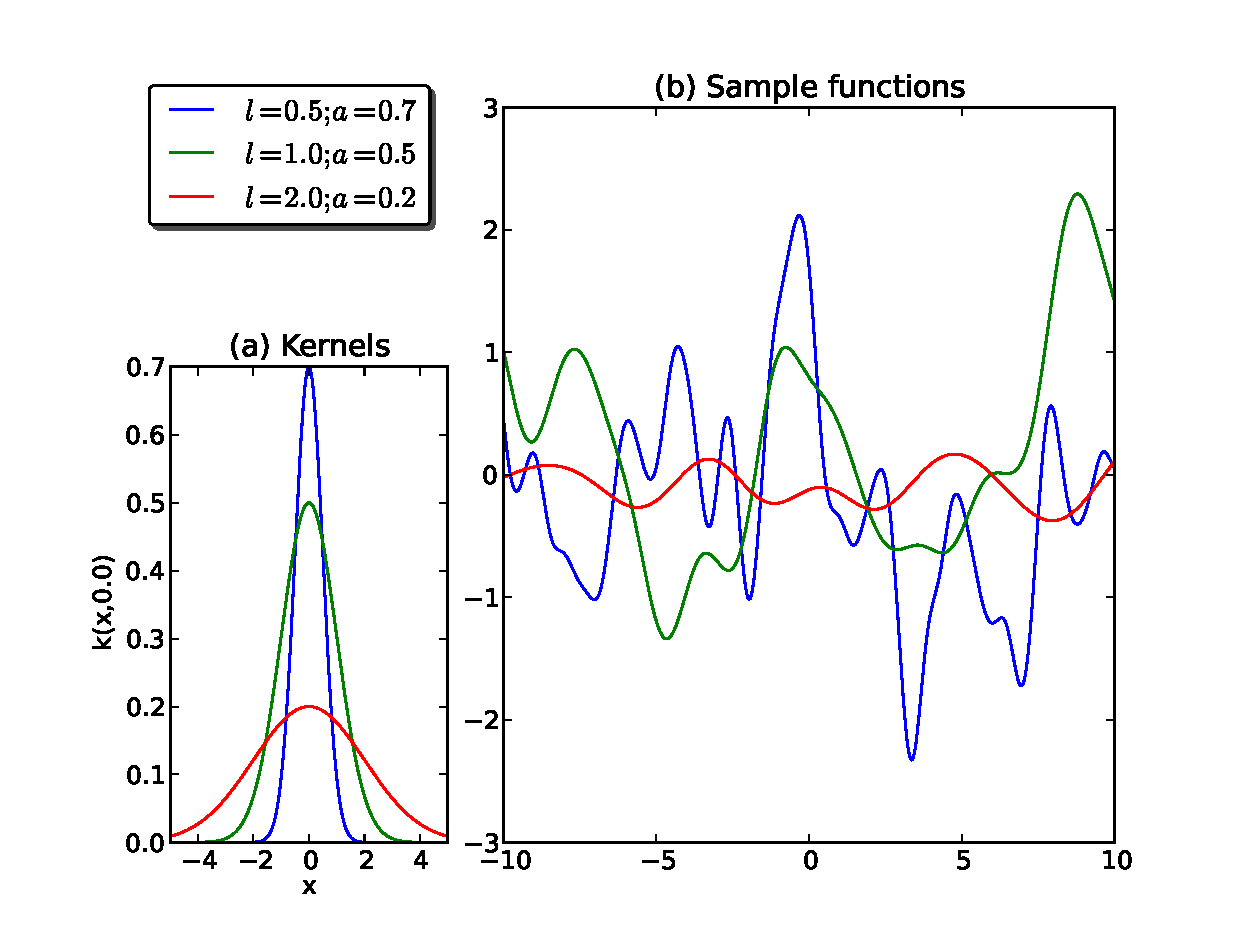
\includegraphics[width=14cm,keepaspectratio]{diagrams/SE_cov.eps}
		\rule{35em}{0.5pt}
	\caption[Exponentiated Quadratic kernel and sample functions]
		{Exponentiated Quadratic kernel and sample functions}
	\label{fig:Exponentiated_Quadratic_covariance}
\end{figure}

Figure \ref{fig:Exponentiated_Quadratic_covariance}$(a)$ represents the kernel and 
Figure \ref{fig:Exponentiated_Quadratic_covariance}$(b)$ shows random sample 
functions drawn from Gaussian process using Exponentiated Quadratic covariance with different
lengthscale and amplitude hyperparameter. The random function was generated for a given input
range by drawing a sample from the multivariate Gaussian using equation \ref{eq:2.2} with zero mean. 
The smoothness of the sample function depends on the equation \ref{eq:EQ_cov}. Function variable
located closer in the input space are highly correlated, whereas function variable located at distance
are loosely correlated or even uncorrelated. Exponentiated Quadratic covariance might be
too smooth to perform any realistic regression task. Depending on the basic nature of the function
other covariance function could be interesting.

\subsection{Rational Quadratic covariance function}

Rational Quadratic covariance function is equivalent to adding together multiple
exponentiated quadratic covariance function having different lengthscale.
Gaussian process prior kernel function expect smooth function with many lengthscale.
Here the parameter $\alpha$ can control the relative weights for lengthscale variations.
Exponentiated quadratic covariance function can be viewed as a special case of rational quadratic 
covariance function. If $\alpha \to \infty$, then both of the functions become identical.
\begin{equation} \label{eq:RQ_cov}
K_{RQ}(r)= a^2 \left(1+ \frac{r^2}{2 \alpha l^2}\right)^{-\alpha}
\end{equation}
where $r=\lVert \textbf{x}-\textbf{x}\textprime \rVert$. 
Figure \ref{fig:Rational_Quadratic_covariance} (a) shows the kernels and (b) shows
three different random sample functions drawn with different setting of hyperparameters 
$a$ and $l$.

\begin{figure}[t]
	\centering
		%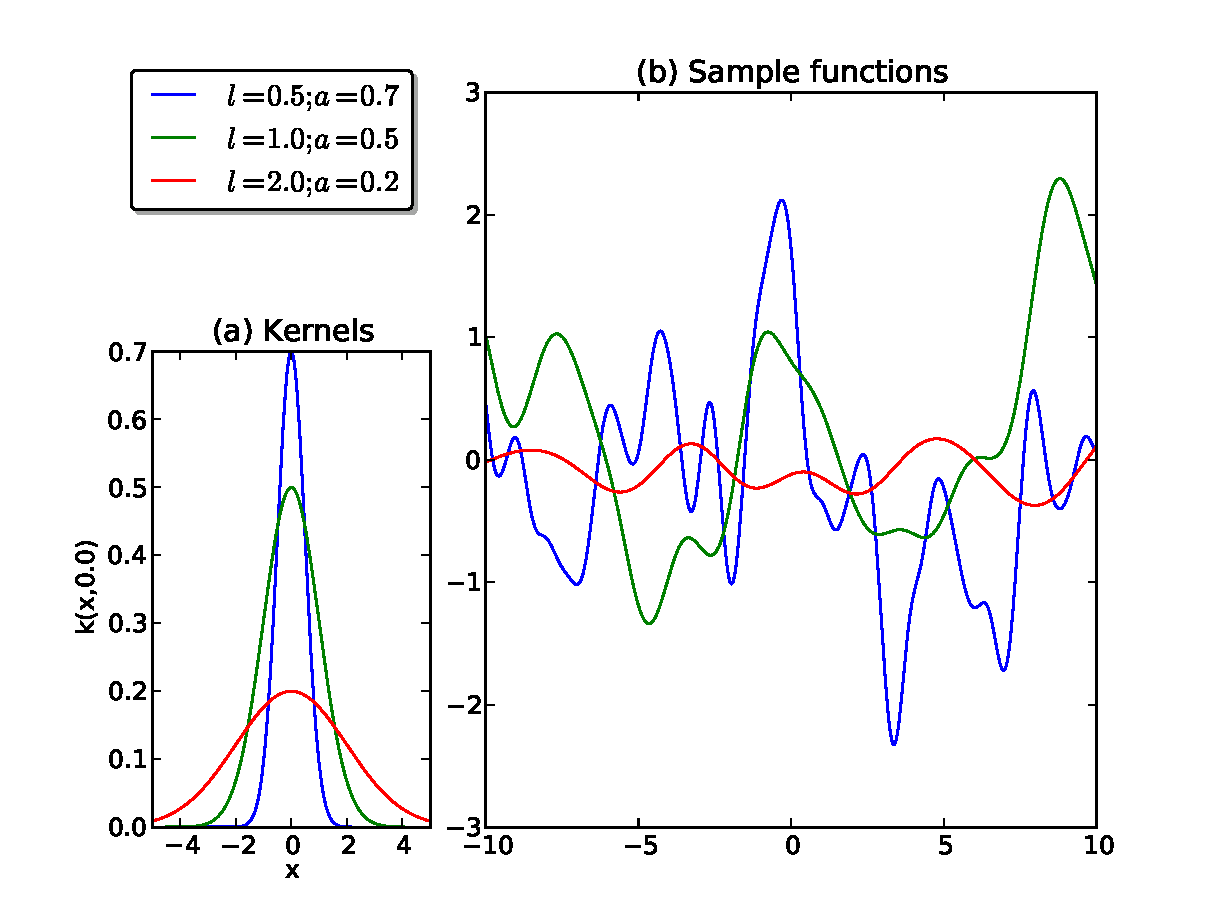
\includegraphics[width=10cm,keepaspectratio]{diagrams/SE_cov.pdf}
		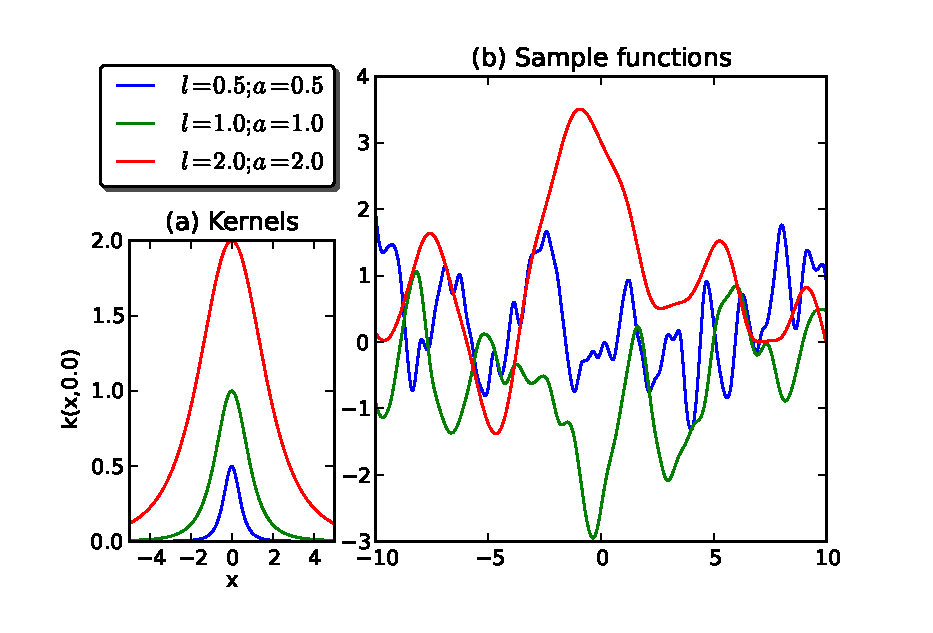
\includegraphics[width=14cm,keepaspectratio]{diagrams/RQ_edit_cov.eps}
		\rule{35em}{0.5pt}
	\caption[Rational Quadratic kernel and random sample functions]
		{Rational Quadratic kernel and random sample functions}
	\label{fig:Rational_Quadratic_covariance}
\end{figure}

\subsection{The Mat{\'e}rn covariance function}
The Mat{\'e}rn class of covariance function are given by equation \ref{eq:Matern_cov}-
\begin{equation} \label{eq:Matern_cov}
K_{Mat}(r)= a^2\frac{2^{1-\nu}}{\Gamma(\nu)}\left(\frac{\sqrt{2\nu}r}{l}\right)^\nu K_{\nu}
	  \left(\frac{\sqrt{2\nu}r}{l}\right)
\end{equation}
where $a, l, \nu$ are positive hyperparameter, $K_{\nu}$ is a modified Bessel function and
$\Gamma \left(.\right)$ is the Gamma function. Hyperparameter $\nu$ controls the roughness 
of the function and as like Exponentiated quadratic covariance function the parameters
$a$ and $l$ controls the amplitude and lengthscale respectively. Though for $\nu \to \infty$
we can obtain the exponentiated quadratic kernel, but for finite value of $\nu$ the sample 
functions are significantly rough. 
\begin{figure}[htbp]
	\centering
		%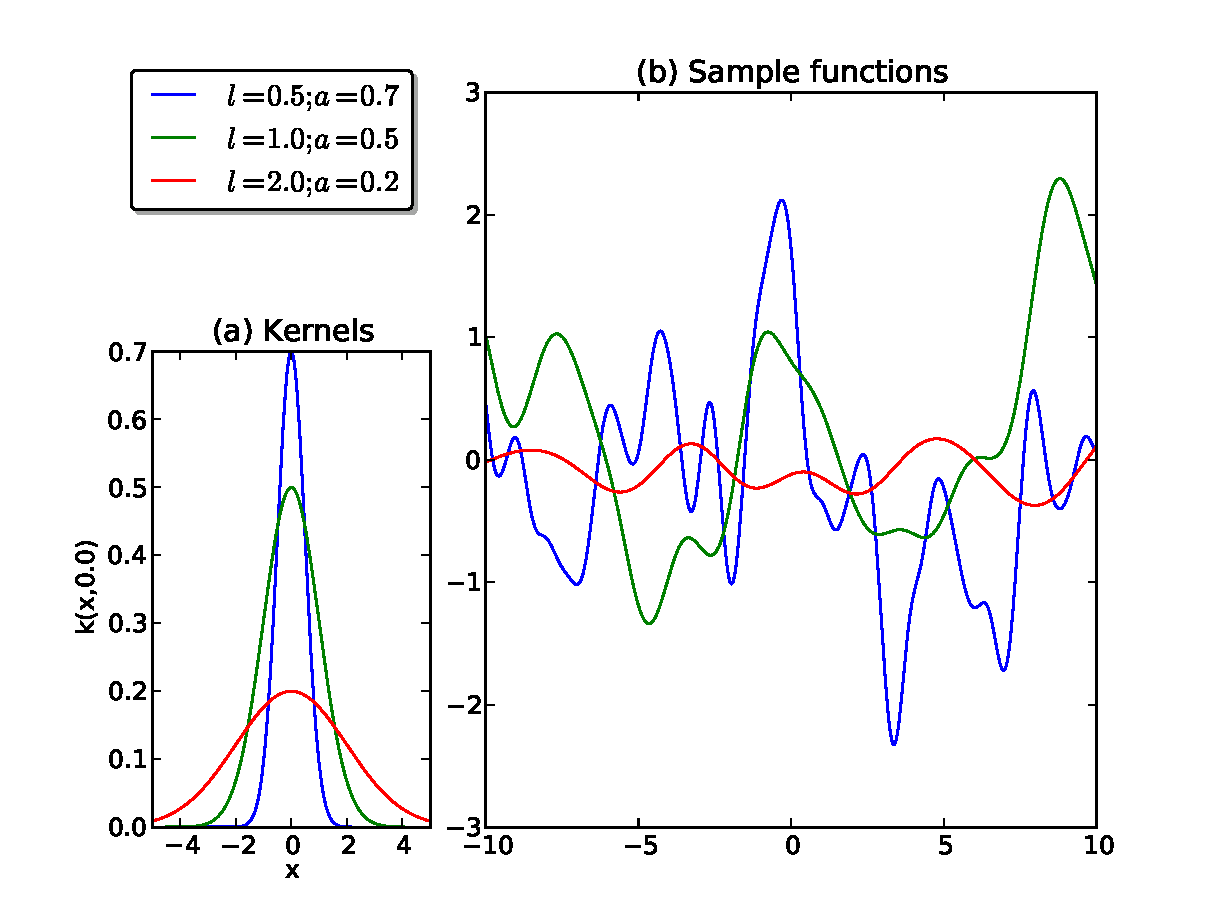
\includegraphics[width=10cm,keepaspectratio]{diagrams/SE_cov.pdf}
		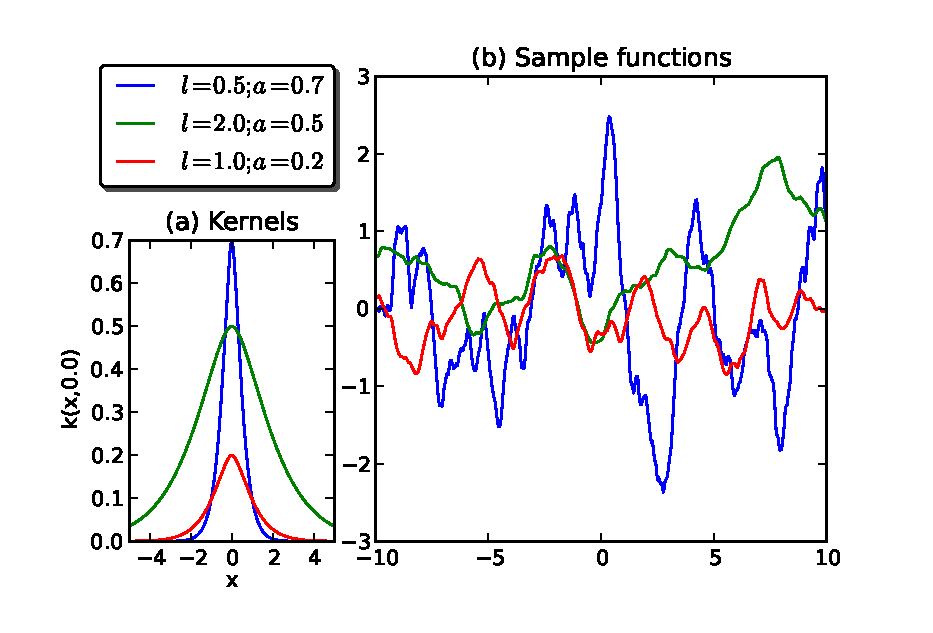
\includegraphics[width=14cm,keepaspectratio]{diagrams/Mat32_cov.eps}
		\rule{35em}{0.5pt}
	\caption[The Mat{\'e}rn32 kernel and random sample functions]
		{The Mat{\'e}rn32 kernel and random sample functions}
	\label{fig:Matern32_covariance}
\end{figure}
The simpler form of Mat{\'e}rn covariance function is obtained when $\nu$ is half integer:
$\nu = p+1/2$, where $p$ is a non-negative integer. The covariance function can be expressed 
as a product of an exponential and a polynomial of order $p$. \cite{Abramowitz:1965} 
derived the general expression as follows-
\begin{equation} \label{eq:MaternGeneral}
K_{\nu=p+1/2}(r)= \exp \left( - \frac{\sqrt{2\nu}r}{l}\right)\frac{\Gamma\left(p+1\right)}{\Gamma\left(2p+1\right)}
		\sum_{i=0}^{p}\frac{\left(p+i\right)!}{i!\left(p-i\right)!}
		\left(\frac{\sqrt{8\nu}r}{l}\right)^{p-i}
\end{equation}
The most interesting cases for machine learning
are $\nu =3/2$ and $\nu=5/2$, for which we get the following equations respectively-
\begin{equation} \label{eq:Matern32}
K_{\nu=3/2}(r)= \left(1+ \frac{\sqrt{3}r}{l} \right)\exp \left( - \frac{\sqrt{3}r}{l} \right)
\end{equation}
\begin{equation} \label{eq:Matern52}
K_{\nu=5/2}(r)= \left(1+ \frac{\sqrt{5}r}{l} + \frac{5r^2}{3l^2} \right)
		\exp \left( - \frac{\sqrt{5}r}{l} \right)
\end{equation}

\subsection{The Ornstein-Uhlenbeck Process}
The Ornstein-Uhlenbeck process (\cite{Ornstein_Uhlenbeck:1930}) is a special case of 
Mat{\'e}rn class covariance functions. The Ornstein-Uhlenbeck process was 
developed as a mathematical model of the velocity of a particle moving with Brownian motion.
\begin{figure}[t]
	\centering
		%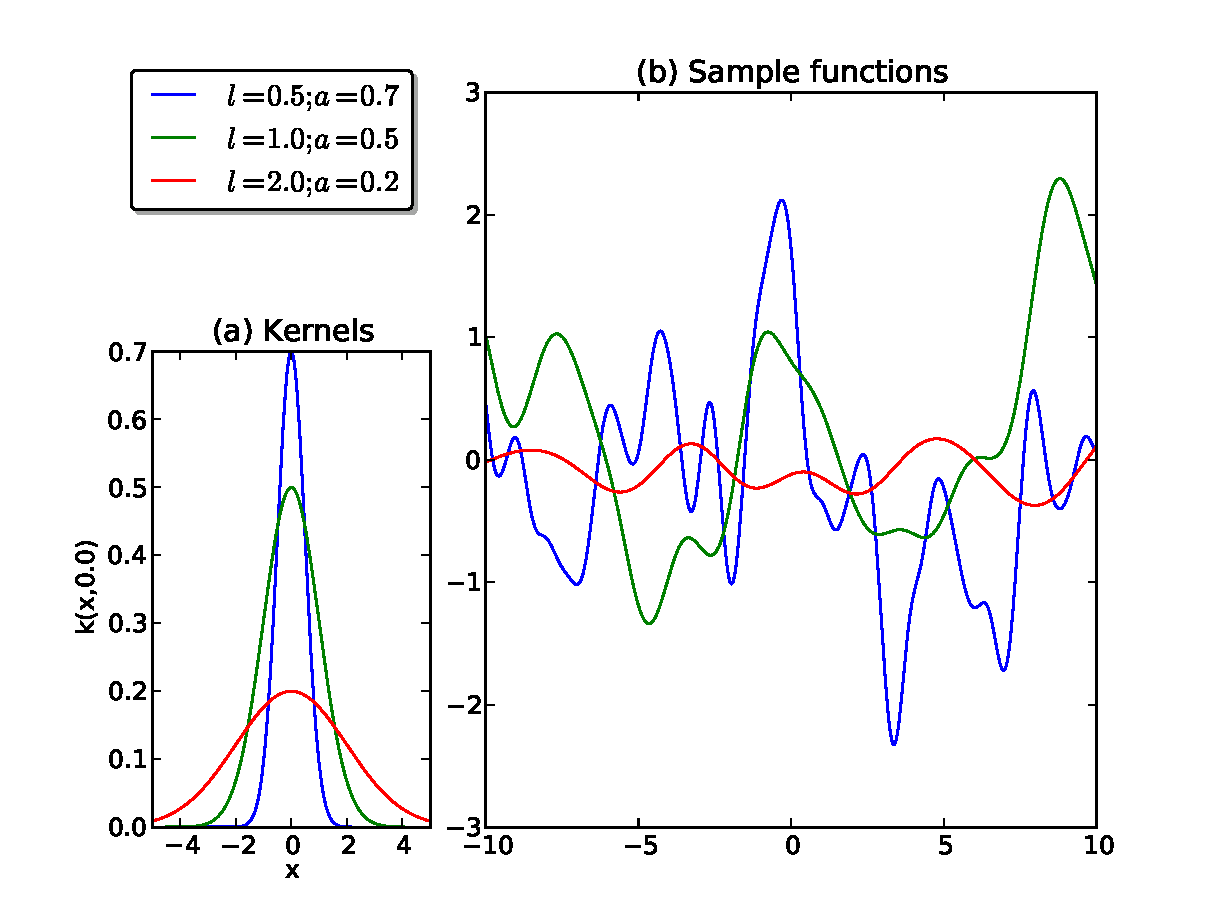
\includegraphics[width=10cm,keepaspectratio]{diagrams/SE_cov.pdf}
		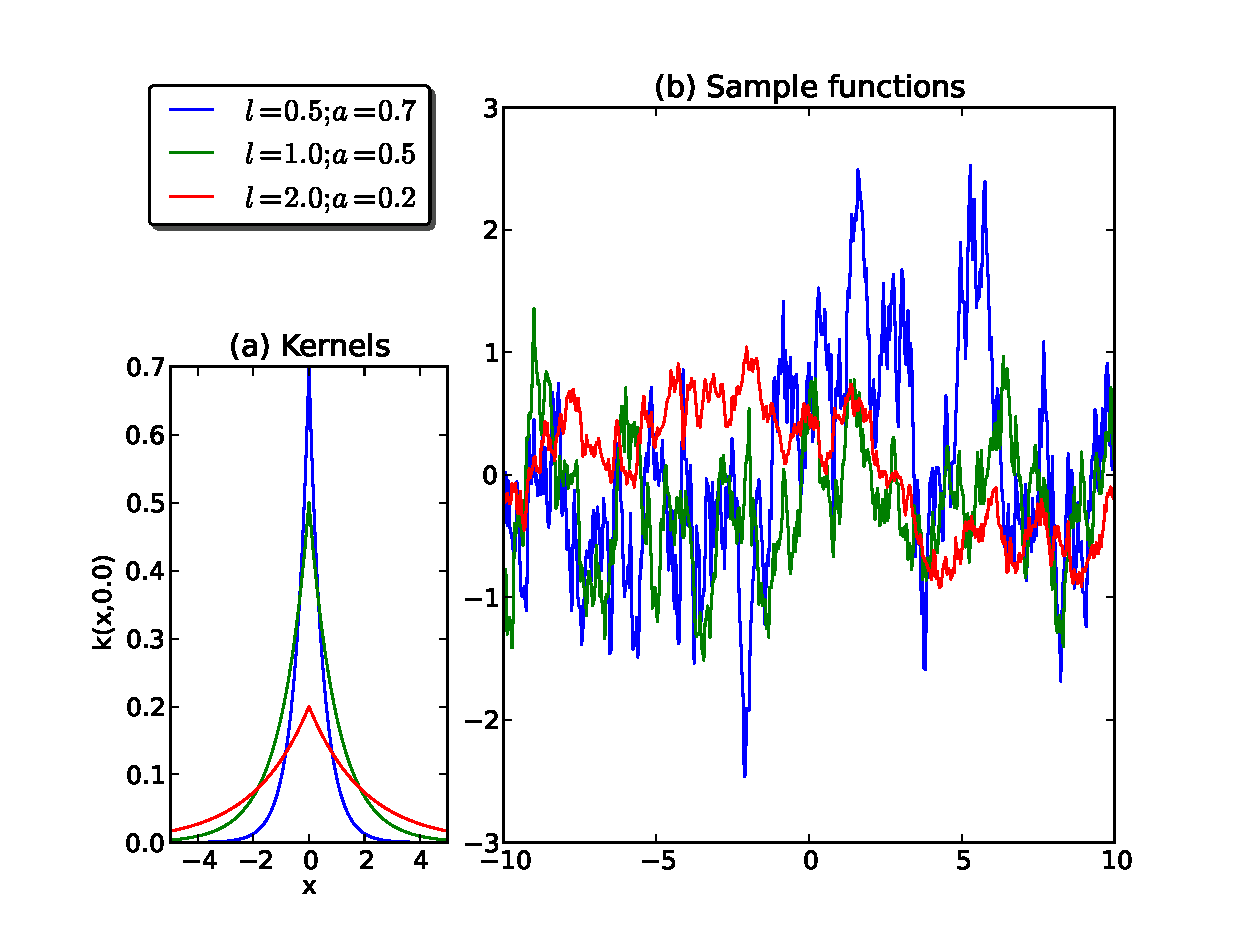
\includegraphics[width=14cm,keepaspectratio]{diagrams/OU_cov.eps}
		\rule{35em}{0.5pt}
	\caption[The OU kernel and random sample functions]
		{The OU kernel and random sample functions}
	\label{fig:OU_covariance}
\end{figure}
The OU process can be found setting up $\nu=1/2$ and expressed as Equation \ref{eq:OU}.
Figure \ref{fig:OU_covariance}$(a)$ shows the kernel and
Figure \ref{fig:OU_covariance}$(b)$ shows the sample functions form the OU process having the 
exactly same amplitude parameter $a$ and lengthscale parameter $l$.  
\begin{equation} \label{eq:OU}
K_{\nu=1/2}(r)=	\exp \left(-\frac{r}{l} \right)
\end{equation}

Figure \ref{fig:DifferentKernels} shows examples of some basic kernels- (a). Exponentiated Quadratic kernel, 
(b). Mat{\'e}rn52 kernel (c). Ornstein-Uhlenbeck kernel (d). Cosine kernel. These kernels are the 
realization of Exponentiated Quadratic covariance function(Equation \ref{eq:EQ_cov}), 
Mat{\'e}rn52 covariance function 
(Equation \ref{eq:Matern52}), Ornstein-Uhlenbeck covariance function (Equation \ref{eq:OU}) 
and Cosine function\footnote{We have not described the Cosine covariance function here. 
The in detail description will be found at \cite{Rasmussen_and_Williams:2006}} respectively.

\begin{figure}[t]
	\centering
		%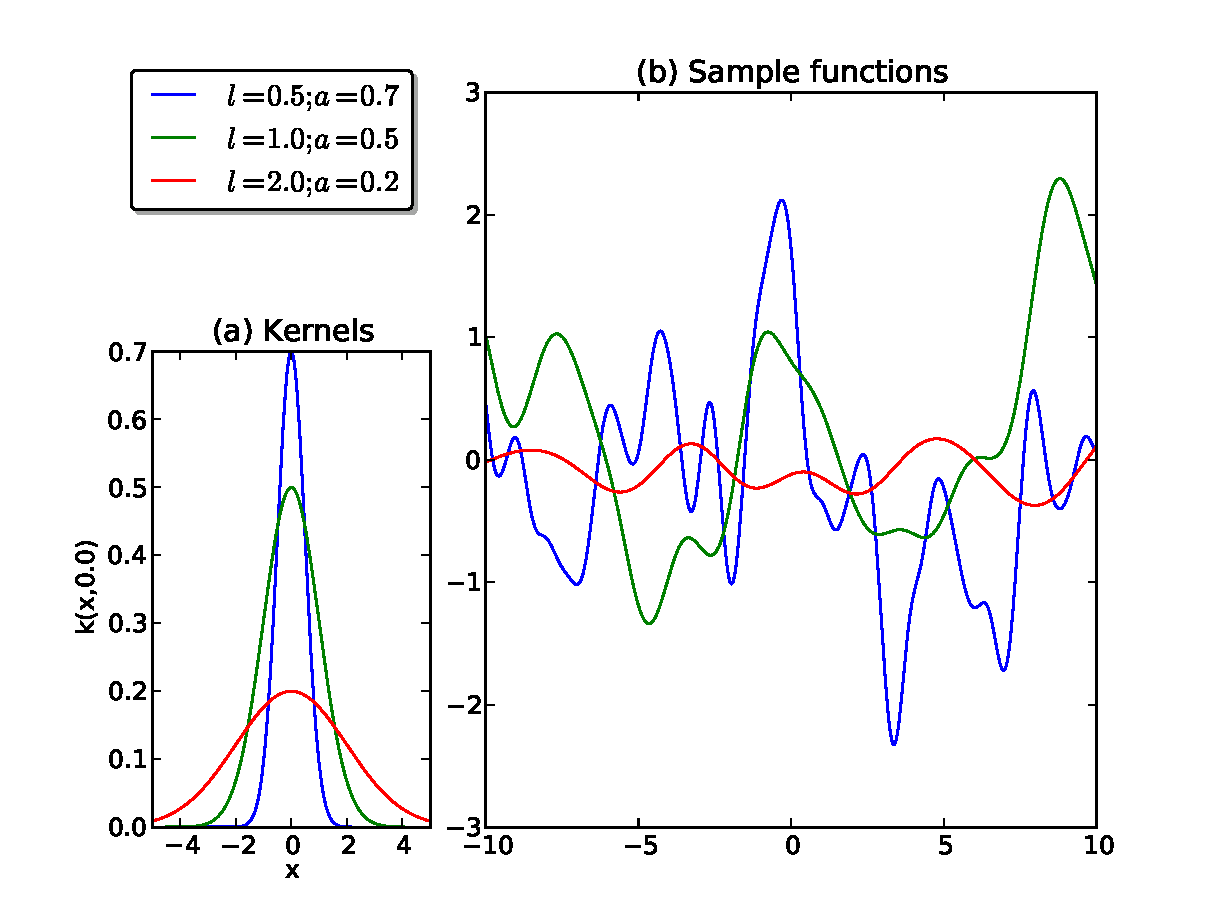
\includegraphics[width=10cm,keepaspectratio]{diagrams/SE_cov.pdf}
		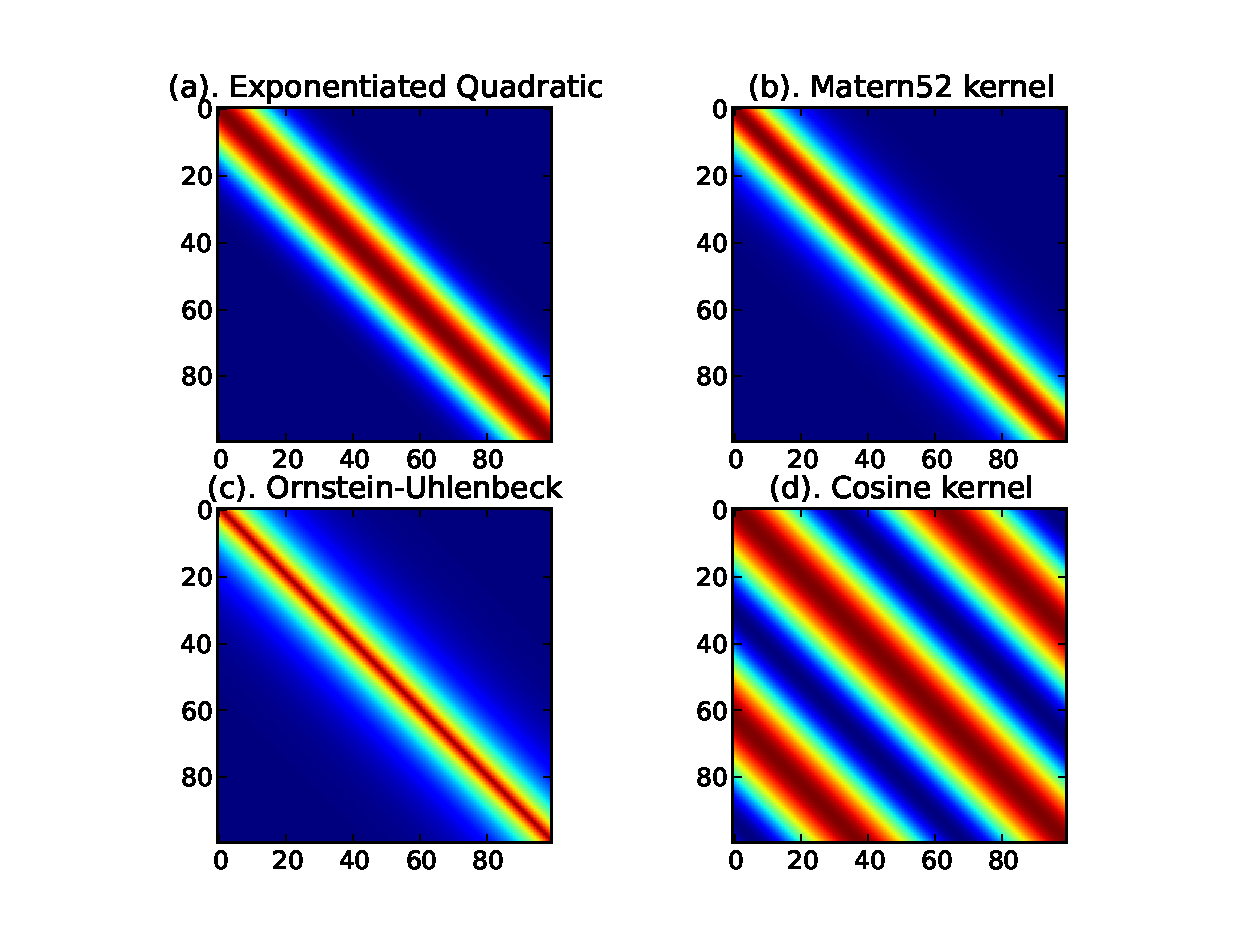
\includegraphics[width=\textwidth,keepaspectratio]{diagrams/DifferentKernels.eps}
		\rule{35em}{0.5pt}
	\caption[Representation of some basic kernels ]
		{Representation of some basic kernels (a). Exponentiated Quadratic kernel, 
		(b). Mat{\'e}rn52 kernel (c). Ornstein-Uhlenbeck kernel (d). Cosine kernel  }
	\label{fig:DifferentKernels}
\end{figure}

\section{Gaussian Process Regression}
Gaussian process regression can be done using the marginal and conditional properties of multivariate
Gaussian distribution. Lets consider that we have some observations $\mathbf{f}$ of a function at observation
point $\mathbf{x}$. Now we wish to predict the values of that function at observation points $\mathbf{x_\star}$,
which we are representing by $\mathbf{f_\star}$. Then the joint probability of $\mathbf{f}$ and $\mathbf{f_\star}$
can be obtained from equation \ref{eq:jointPro_f_f*}-

\begin{equation} \label{eq:jointPro_f_f*}
p \left( \begin{bmatrix} \mathbf{f} \\\mathbf{f_\star} \end{bmatrix} \right) =
\mathcal{N}\left( \begin{bmatrix} \mathbf{f} \\\mathbf{f_\star} \end{bmatrix} \middle|
\mathbf{0}, \begin{bmatrix} \mathbf{K_{x,x}} & \mathbf{K_{x,x_\star}} \\
			    \mathbf{K_{x_\star,x}} & \mathbf{K_{x_\star,x_\star}} \end{bmatrix} \right)
\end{equation}

where the covariance matrix $ \mathbf{K_{x,x}}$ has elements derived from the covariance function 
$ k \left(x,x\textprime \right)$, such that the $ \left(i,j \right)^{th}$ element of $ \mathbf{K_{x,x}}$ is
given by $k \left( \mathbf{x} \left[ i\right],\mathbf{x} \left[ i\right] \right) $ 
The conditional property of a multivariate Gaussian is used to perform regression the. The conditional
property is can be represented by the equation \ref{eq:condProMvG}: 

\begin{equation} \label{eq:condProMvG}
p \left( \mathbf{f} \middle| \mathbf{f_\star} \right) =
\mathcal{N}\left( \mathbf{f_\star} \middle| \mathbf{K_{x_\star,x}}  \mathbf{K^{-1}_{x,x}} \mathbf{f,} \mathbf{K_{x_\star,x_\star}} - 
\mathbf{K_{x_\star,x}} \mathbf{K^{-1}_{x,x}} \mathbf{K_{x,x_\star}}\right)
\end{equation}

In ideal case the observations $\mathbf{f}$ is noise free but in practice it is always corrupted with some noise.
Lets consider $\mathbf{y}$ is the corrupted version of $\mathbf{f}$. If we consider this noise as Gaussian noise
then we can write $p \left( \mathbf{y} \middle| \mathbf{f} \right) = \mathcal{N} \left( \mathbf{y} \middle| \mathbf{f},
\sigma^2 \mathbf{I} \right) $, where $ \sigma^2 $ is the variance of the noise and $\mathbf{I}$ is the identity
matrix with appropriate size and marginalise the observation $\mathbf{f}$. Then the joint probability of 
$\mathbf{y}$ and $\mathbf{f_\star}$ can be represented by the equation \ref{eq:jointPro_y_f*}.

\begin{equation} \label{eq:jointPro_y_f*}
p \left( \begin{bmatrix} \mathbf{y} \\\mathbf{f_\star} \end{bmatrix} \right) =
\mathcal{N}\left( \begin{bmatrix} \mathbf{y} \\\mathbf{f_\star} \end{bmatrix} \middle|
\mathbf{0}, \begin{bmatrix} \mathbf{K_{x,x}}+ \sigma^2\mathbf{I} & \mathbf{K_{x,x_\star}} \\
			    \mathbf{K_{x_\star,x}} & \mathbf{K_{x_\star,x_\star}} \end{bmatrix} \right)
\end{equation}

Regression with Gaussian process is Bayesian method. From the knowledge of a $prior$ over a function we proceed to a
$posterior$ and this happens in a closed from of equation \ref{eq:condProMvG}. 

\begin{figure}[t]
	\centering
		%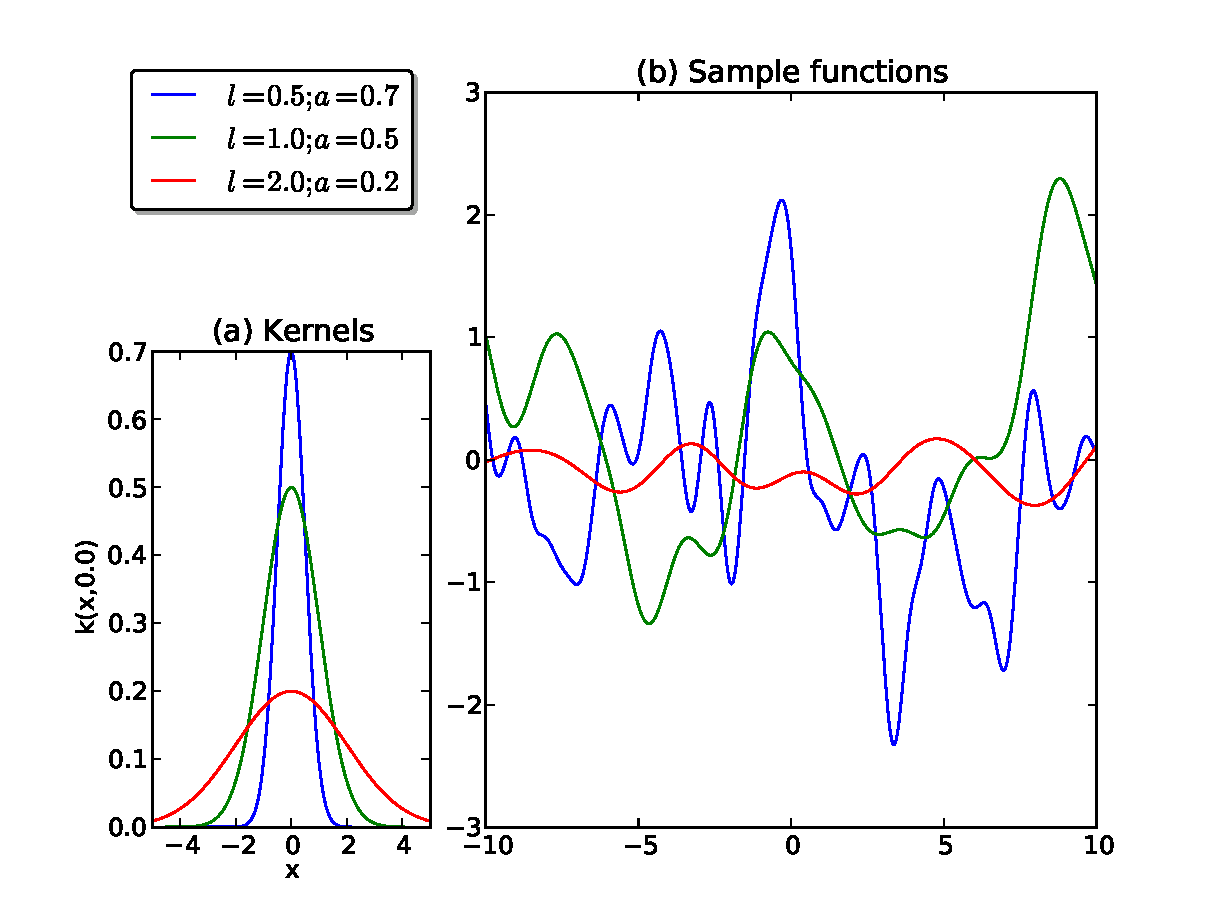
\includegraphics[width=10cm,keepaspectratio]{diagrams/SE_cov.pdf}
		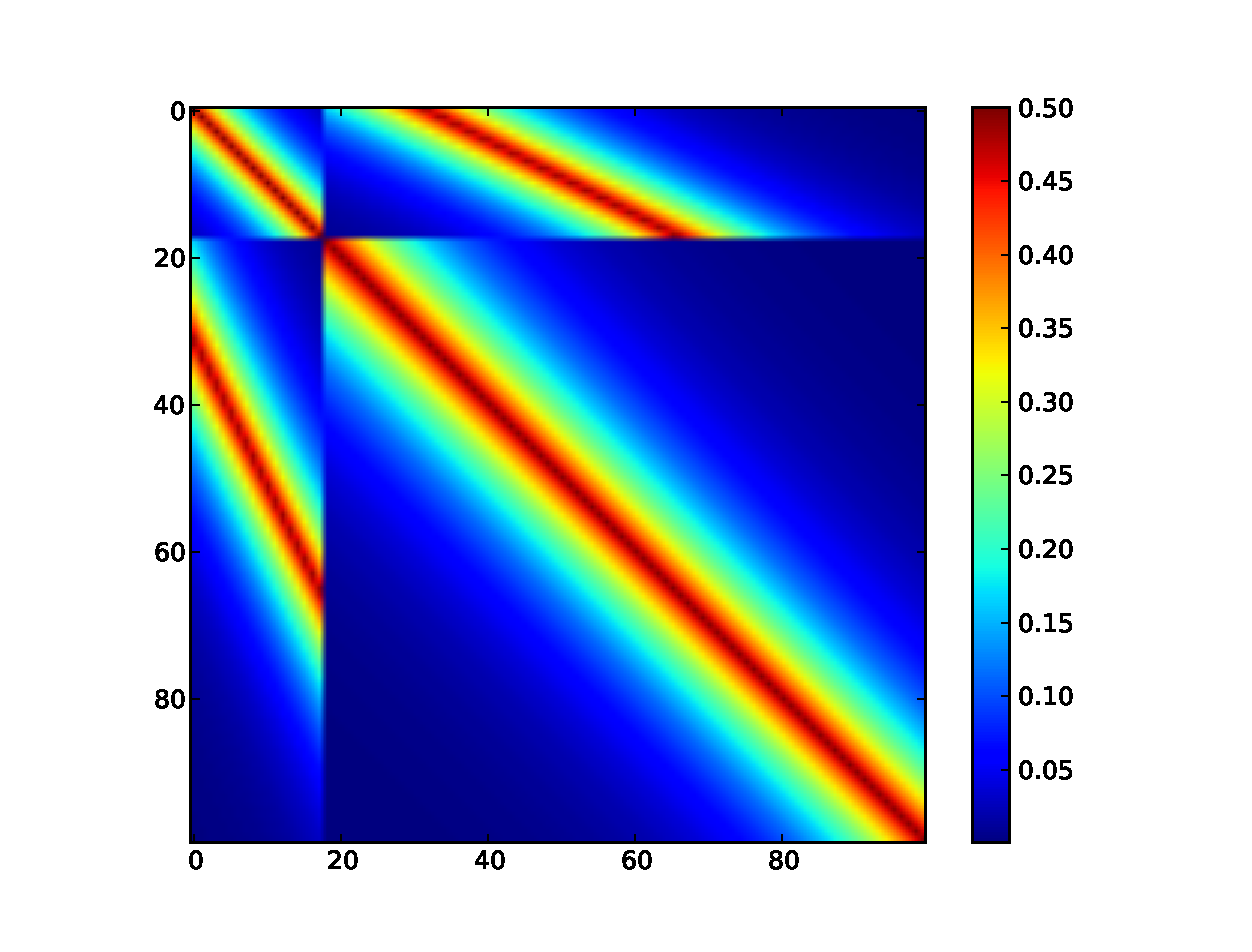
\includegraphics[width=0.8\textwidth,keepaspectratio]{diagrams/Cov_Structure.eps}
		\rule{35em}{0.5pt}
	\caption[Overall representation of covariances between training and test data]
		{Overall representation of covariances between training and test data}
	\label{fig:Covariances_Structure}
\end{figure}

Figure \ref{fig:Covariances_Structure} shows the overall covariance structure between some training and test data.
For this example we choose 18 training points and 82 test points. We observed the shaded structure because some of
the training data are closer to some of the test data. Observing this structure we can also figure out the closeness
between training and test data. 

\subsection{Making prediction}
The probability density is represented by functions. Due to consistency this density is known as a process. Also by this
property, any future values of $\mathbf{f_\star}$ which are unobserved can be predicted without affecting $\mathbf{f}$.
To make prediction of the test data we use the conditional distribution. In ideal case the conditional distribution
is $ p\left( \mathbf{f_\star} \middle| \mathbf{f} \right) $ and if we consider the noise then the conditional distribution
will be $ p\left( \mathbf{f_\star} \middle| \mathbf{y} \right) $. Both of the distribution are also Gaussian,
\begin{equation} \label{eq:prediction}
  \mathbf{f_\star}  \sim \left( \boldsymbol{\mu}_f, \mathbf{C}_f \right)
\end{equation}

The mean of the conditional distribution of Equation \ref{eq:prediction} is:
\begin{equation} \label{eq:prediction_mean}
  \boldsymbol{\mu}_f = \mathbf{K_{x,x_\star}^T} \left[ \mathbf{K_{x,x}}+ \sigma^2\mathbf{I} \right]^{-1} \mathbf{y}
\end{equation}

and the covariance of the conditional distribution of Equation \ref{eq:prediction} given by:
\begin{equation} \label{eq:prediction_cov}
  \mathbf{C}_f = \mathbf{K_{x_\star,x_\star}} -
		\mathbf{K_{x,x_\star}^T} \left[ \mathbf{K_{x,x}}+ \sigma^2\mathbf{I} \right]^{-1} \mathbf{K_{x,x_\star}}
\end{equation}

These results can be calculated using block matrix inverse rules. The derivation can found 
in appendix section (Appendix \ref{AppendixA}). Figure \ref{fig:dempGPReg} shows a simple example of regression
using Gaussian process.

\begin{figure}[t]
	\centering
		%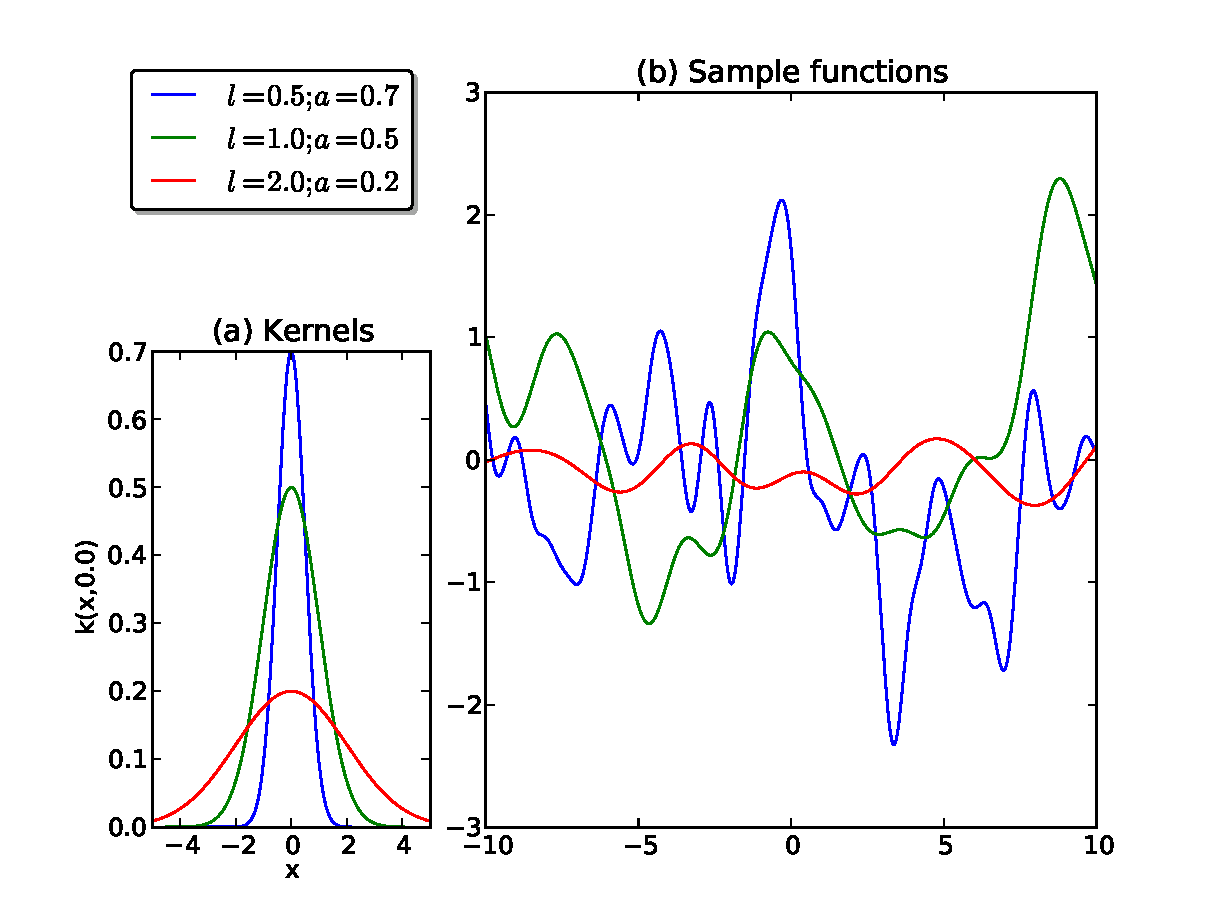
\includegraphics[width=10cm,keepaspectratio]{diagrams/SE_cov.pdf}
		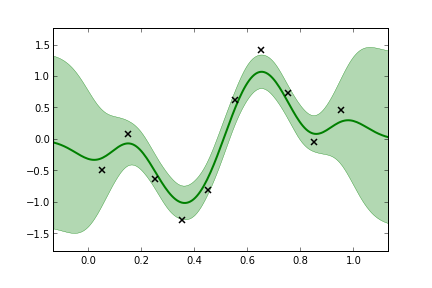
\includegraphics[width=10cm,keepaspectratio]{diagrams/demoGPReg.png}
		\rule{35em}{0.5pt}
	\caption[Simple example of regression using Gaussian process]
		{Simple example of regression using Gaussian process}
	\label{fig:dempGPReg}
\end{figure}

\subsection{Hyperparameter Learning}
To construct the covariance function
still we need to consider the hyperparameters and optimize those. The most efficient and commonly used 
optimization technique for hyperparameters can be done using maximum likelihood. If we consider all the hyperparameters
$\alpha$, $\sigma^2$ and $l$ in to a vector $\boldsymbol{\theta}$, then we can use gradient methods to optimize
$p \left(\mathbf{y}\middle|\boldsymbol{\theta}\right)$ with respect to $\boldsymbol{\theta}$. The Log
likelihood is given by:

\begin{equation} \label{eq:Likelihood}
 p \left(\mathbf{y}\middle|\boldsymbol{\theta}\right) =
    - \frac{D}{2}log2\pi - \frac{1}{2}\times log \left| \mathbf{K_{x,x}} + \sigma^2\mathbf{I}\right|
    - \frac{1}{2}\mathbf{y}^T \left[\mathbf{K_{x,x}} + \sigma^2\mathbf{I} \right]^{-1}\mathbf{y}
\end{equation}

We can have the Log maximum likelihood by:
\begin{equation} \label{eq:LML}
 \boldsymbol{\theta}_{max} = argmax \left( p\left(\mathbf{y}\middle|\boldsymbol{\theta}\right) \right)
\end{equation}

\section{Toward the GP model of TFA}
Simo S\"arkk\"a indicated an analogical pathway \footnote{Not published yet, came through some discussions}
to construct a kernel function for Gaussian process from
Markovian assumption based probabilistic approach of \cite{Sanguinetti:2006}.
In the earlier probabilistic approach gene specific TFAs was obtained from-
\begin{equation} \label{eq:tfa_SanG_updateCh4}
  \bold{b}_{n(t+1)} \sim \mathcal{N} (\gamma \bold{b}_{nt} + (1-\gamma)\boldsymbol{\mu},(1-\gamma^2)\bold{\Sigma})
\end{equation}
For a discrete time variable $k$ the above equation can be rewrite as-
\begin{equation}
\textbf{b}_{n(k+1)} \sim \mathcal{N}\left(\gamma \textbf{b}_{nk} + (1 - \gamma) \boldsymbol{\mu}, (1 - \gamma^2) \boldsymbol{\Sigma}\right),
\end{equation}
and
\begin{equation}
\textbf{b}_{n_1} \sim \mathcal{N}\left(\boldsymbol{\mu}, \boldsymbol{\Sigma}\right)
\end{equation}
Let's now form a continuous model which has these same finite-dimensional distributions. 
First construct a one-dimensional process with the property-
\begin{equation}
u_{k+1} \sim \mathcal{N}\left(\gamma u_k + \left(1 - \gamma\right) \mu, (1 - \gamma^2)s \right),
\end{equation}
where $\mu$ and $s$ are scalar.

We can now assume that $u_k$'s are actually values $u_{t_k}$ from a continuous process $u(t)$ and  
let's assume that- 
\begin{equation}
t_k = kDt.
\end{equation}

A good candidate for this kind of model is the mean-reverting $Ornstein-Uhlenbeck$ model 
(\cite{Ornstein_Uhlenbeck:1930})-
\begin{equation}
du = -\lambda \left(u - \mu\right) dt + q^{1/2} dB,
\end{equation}
where $B$ is a standard Brownian motion (i.e., Wiener process). 
This equation can now be solved on the time instants $t_k$ and the result is a recursion
\begin{equation}
u(t_k) = a u(t_{k-1}) + b \mu + w_{k-1},
\end{equation}
where $w_{k-1} \sim \mathcal{N}(0,c)$ with-\\
$a = \exp(-\lambda Dt)$\\~\\
$b = \int_0^Dt \exp(-\lambda (Dt-s)) ds\\
 = 1 - \exp(-\lambda Dt)$\\~\\
$c = \int_0^Dt \exp(-\lambda (Dt-s)) q \exp(-\lambda (Dt-s)) ds \\
= q \int_0^Dt \exp(-2 \lambda (Dt-s)) ds\\
= [q / (2 \lambda)] [1 - \exp(-2 \lambda Dt)]$

That is,
\begin{equation}
u_{k+1} \sim \mathcal{N}\left(a u_k + b \mu, c\right).
\end{equation}

We can now match the coefficients:
\begin{equation} \label{eq:a}
a = \exp(-\lambda Dt) = \gamma
\end{equation}
\begin{equation} \label{eq:b}
b = 1 - \exp(-\lambda Dt) = 1 - \gamma
\end{equation}
\begin{equation} \label{eq:c}
c = (1 - \gamma^2) s = [q / (2 \lambda)] [1 - \exp(-2 \lambda Dt)]
\end{equation}

Equation \ref{eq:a} quite luckily has a nice solution 
$\gamma = \exp(-\lambda Dt)$ and from Equation \ref{eq:c} we will have another solution
$s = q / (2 \lambda)$,
which can be inverted to give
$\lambda = -[1 / Dt] \log \gamma$ and
$q = -[2 s / Dt] \log \gamma$. 

If we arbitrarily fix $Dt = 1$, we get
$\lambda = -\log \gamma$\\
$q = -2 s \log \gamma$.

We can now recall that the (stationary) covariance function of the Ornstein-Uhlenbeck process we get-

$k_u(t,t')
  = [q / (2 \lambda)] \exp(-\lambda {\left|t-t'\right|})\\
  = s \exp((\log \gamma) {\left|t-t'\right|})\\
  = s \exp({\left|t-t'\right|}(\log \gamma))\\
  = s \exp(\log \gamma^{\left|t-t'\right|})\\
  = s \gamma^{\left|t-t'\right|}$.

When we start from variance $s = q / \left[2 \lambda\right]$, then the process will indeed be stationary 
from the start. Returning to the original vector valued $\textbf{b}$, because the system is separable, we can 
conclude that the implied covariance function is just obtained by formally replacing $s$ with 
$\boldsymbol{\Sigma}$ everywhere- 
\begin{equation}
\textbf{K}_b(t,t') = \boldsymbol{\Sigma} \boldsymbol{\gamma}^{\left|t-t'\right|}
\end{equation}

Thus is equivalent to considering the vector process of mean-reverting $Ornstein-Uhlenbeck$ model
\begin{equation}
\textbf{db} = -\lambda (\textbf{b} - \boldsymbol{\mu}) \textbf{dt} + Q^{1/2} \textbf{dB}.
\end{equation} 
% Chapter 5

\chapter{Gaussian Process Model of Gene Expressions} % Main chapter title

\label{Chapter5} % For referencing the chapter elsewhere, use \ref{Chapter1} 
\lhead{Chapter 5. \emph{Gaussian Process Model of Gene Expressions}} % This is for the header on each page - perhaps a shortened title
%\lhead{Chapter 5. \emph{Ranking Differentially Expressed C Elegans Gene Expressions}} % This is for the header on each page - perhaps a shortened title

%----------------------------------------------------------------------------------------

%\section{Ranking...}

In this chapter we design a covariance function for reconstructing transcription factor activities given gene 
expression profiles and a connectivity matrix (binding data) between genes and transcription factors. 
Our modelling framework builds on ideas of \cite{Sanguinetti:2006} 
who used a linear-Gaussian state-space modelling framework to infer the transcription factor activity 
of a group of genes. 

We note that the linear Gaussian model is equivalent to a Gaussian process with a particular covariance function. 
We therefore build a model directly from the Gaussian process perspective to achieve the same effect. 
We introduce a computational trick, based on  judicious application of singular value decomposition, 
to enable us to efficiently fit the Gaussian process in a reduced 'TF activity' space. 

%----------------------------------------------------------------------------------------

First we load in the classic \cite{Spellman:1998} Yeast Cell Cycle data set. The cdc15 time series data has 
23 time points. We can load this gene expression data in with GPy.

Time series of synchronized yeast cells from the CDC-15 experiment of \cite{Spellman:1998}. 
Two colour spotted cDNA array data set of a series of experiments to identify which genes in Yeast are 
cell cycle regulated.
We can make a simple helper function to plot genes from the data set (which are provided as a pandas array).

Our second data set is from ChiP-chip experiments performed on yeast by \cite{Lee:2002}. 
These give us the binding information between transcription factors and genes. 
In this notebook we are going to try and combine this binding information with 
the gene expression information to infer transcription factor activities.

\section{Model for Transcription Factor Activities}

We are working with $log$ expression levels in a matrix $\mathbf{Y} \in \Re^{n\times T}$ and 
we will assume a linear (additive) model giving the relationship between the expression level 
of the gene and the corresponding transcription factor activity which are unobserved, but we 
represent by a matrix $\mathbf{F} \in \Re^{q\times T}$. Our basic assumption is as follows. 
Transcription factors are in time series, so they are likely to be temporally smooth. 
Further we assume that the transcription factors are potentially correlated with one another 
(to account for transcription factors that operate in unison). 

\textbf{Correlation Between Transcription Factors}:  
If there are $q$ transcription factors then the correlation between different transcription factors is 
encoded in a covariance matrix, $\boldsymbol{\Sigma}$ which is $q\times q$ in dimensionality. 

\textbf{Temporal Smoothness}: 
Further we assume that the log of the transcription factors' activities is temporally smooth, 
and drawn from an underlying Gaussian process with covariance $\mathbf{K}_t$. 

\textbf{ Intrinsic Coregionalization Model}: 
We assume that the joint process across all $q$ transcription factor activities and across all time points 
is well represented by an intrinsic model of coregionalization where the covariance is given by the 
Kronecker product of these terms.
\begin{equation} \label{eq:K}
  \mathbf{K}_f = \mathbf{K}_t \otimes \boldsymbol{\Sigma}
\end{equation}

This is known as an intrinsic coregionalization model (\cite{Wackernagel:2003}). 
\cite{Alvarez:2012} presented the machine learning orientated review of these methods. 
The matrix $\boldsymbol{\Sigma}$ is known as the coregionalization matrix.

\section{Relation to Gene Expressions}

We now assume that the $j$th gene's expression is given by the product of the transcription factors that bind to 
that gene. Because we are working in log space, that implies a log linear relationship. At the $i$th time point, 
the log of the $j$th gene's expression, $\mathbf{y}_{i,j}$ is linearly related to the log of the transcription 
factor activities at the corresponding time point, $\mathbf{f}_{i, :}$. This relationship is given by the binding 
information from $\mathbf{S}$. We then assume that there is some corrupting Gaussian noise to give us the final 
observation.
\begin{equation} \label{eq:yij}
  \mathbf{y}_{i, j} = \mathbf{S}\mathbf{f}_{:, i} + \boldsymbol{\epsilon}_i
\end{equation}  
where the Gaussian noise is sampled from
\begin{equation} \label{eq:epsi}
  \epsilon_i \sim \mathcal{N}(\mathbf{0}, \sigma^2 \mathbf{I})
\end{equation}

\section{Gaussian Process Model of Gene Expression}

We consider a vector operator which takes all the separate time series in $\mathbf{Y}$ and stacks the time series 
to form a new vector $n\times T$ length vector $\mathbf{y}$. A similar operation is applied to form a $q \times T$ 
length vector $\mathbf{f}$. Using Kronecker products we can now represent the relationship between $\mathbf{y}$ and 
$\mathbf{f}$ as follows:  
Standard properties of multivariate Gaussian distributions tell us that
\begin{equation} \label{eq:mGPd}
\mathbf{y} \sim \mathcal{N}(\mathbf{0}, \mathbf{K}),
\end{equation}
where
\begin{equation} \label{eq:K}
\mathbf{K} = \mathbf{K}_t \otimes \mathbf{S} \boldsymbol{\Sigma} \mathbf{S}^\top + \sigma^2 \mathbf{I}.
\end{equation}
This results in a covariance function that is of size $n$ by $T$ where $n$ is number of genes and $T$ is number of 
time points. However, we can get a drastic reduction in the size of the covariance function by considering 
the singular value decomposition of $\mathbf{S}$. 
The matrix $\mathbf{S}$ is $n$ by $q$ matrix, where $q$ is the number of transcription factors. It contains a 1 
if a given transcription factor binds to a given gene, and zero otherwise. 
The likelihood of a multivariate Gaussian is:
\begin{equation} \label{eq:Likelihood}
L = -\frac{1}{2} \log |\mathbf{K}| - \frac{1}{2} \mathbf{y}^\top \mathbf{K}^{-1} \mathbf{y}
\end{equation}

In the worst case, because the vector $\mathbf{y}$ contains $T\times n$ points ($T$ time points for 
each of $n$ genes) we are faced with $O(T^3n^3)$ computational complexity. We are going to use a rotation trick to 
get the likelihood. 

\section{The Main Computational Trick}

\subsection{Rotating the Basis of a Multivariate Gaussian}
For any multivariate Gaussian you can rotate the data set and compute a new rotated covariance which is valid for the 
rotated data set. Mathematically this works by first inserting $\mathbf{R}\mathbf{R}^\top$ into the likelihood at 
three points as follows:
\begin{equation} \label{eq:LikelihoodRotation}
  L = -\frac{1}{2} \log |\mathbf{K}\mathbf{R}^\top\mathbf{R}| 
      - \frac{1}{2} \mathbf{y}^\top\mathbf{R}^\top\mathbf{R} \mathbf{K}^{-1}\mathbf{R}^\top\mathbf{R} \mathbf{y} 
      + \text{const}
\end{equation}
The rules of determinants and a transformation of the data allows us to rewrite the likelihood as
\begin{equation} \label{eq:LikelihoodRotationRerite}
  L = -\frac{1}{2} \log |\mathbf{R}^\top\mathbf{K}\mathbf{R}| 
      - \frac{1}{2} \hat{\mathbf{y}}^\top \left[\mathbf{R}^\top\mathbf{K}\mathbf{R}\right]^{-1}\hat{\mathbf{y}} 
      + \text{const}
\end{equation}
where we have introduced the rotated data: $\hat{\mathbf{y}}=\mathbf{R} \mathbf{y}$. 
Geometrically what this says is that if we want to maintain the same likelihood, then when we rotate our data set by 
$\mathbf{R}$ we need to rotate either side of the covariance matrix by $\mathbf{R}$, which makes perfect sense 
when we recall the properties of the multivariate Gaussian. 

\subsection{A Kronecker Rotation}
In this paper we are using a particular structure of covariance which involves a Kronecker product. 
The rotation we consider will be a Kronecker rotation (\cite{Stegle:2011}). 
We are going to try and take advantage of the fact that the matrix $\mathbf{S}$ is square meaning that 
$\mathbf{S}\boldsymbol{\Sigma}\mathbf{S}^\top$ is not full rank (it has rank of most $q$, but is size $n\times n$, and 
we expect number of transcription factors $q$ to be less than number of genes $n$). 

When ranks are involved, it is always a good idea to look at singular value decompositions (SVDs). The SVD of 
$\mathbf{S}$ is given by:
\begin{equation} \label{eq:SVD}
\mathbf{S} = \mathbf{Q} \boldsymbol{\Lambda} \mathbf{V}^\top
\end{equation}
where $\mathbf{V}^\top \mathbf{V} = \mathbf{I}$, $\boldsymbol{\Lambda}$ is a diagonal matrix of positive values, 
$\mathbf{Q}$ is a matrix of size $n\times q$: it matches the dimensionality of $\mathbf{S}$, but we have 
$\mathbf{Q}^\top \mathbf{Q} = \mathbf{I}$. Note that because it is not square, $\mathbf{Q}$ is not in itself a 
rotation matrix. However it could be seen as the first $q$ columns of an $n$ dimensional rotation matrix 
(assuming $n$ is larger than $q$, i.e. there are more genes than transcription factors). 

If we call the $n-q$ missing columns of this rotation matrix $\mathbf{U}$ then we have a valid rotation matrix 
$\mathbf{R}=\begin{bmatrix} \mathbf{Q}& \mathbf{U}\end{bmatrix}$. Although this rotation matrix is only rotating 
across the $n$ dimensions of the genes, not the additional dimensions across time. In other words we are choosing 
$\mathbf{K}_t$ to be unrotated. To represent this properly for our covariance we need to set 
$\mathbf{R} = \mathbf{I} \otimes \begin{bmatrix} \mathbf{Q}& \mathbf{U}\end{bmatrix}$. This gives us a structure 
that when applied to a covariance of the form $\mathbf{K}_t\otimes \mathbf{K}_n$ it will rotate $\mathbf{K}_n$ 
whilst leaving $\mathbf{K}_t$ untouched.

When we apply this rotation matrix to $\mathbf{K}$ we have to consider two terms, 
the rotation of $\mathbf{K}_t \otimes \mathbf{S}\boldsymbol{\Sigma}\mathbf{S}^\top$, 
and the rotation of $\sigma^2 \mathbf{I}$.

Rotating the latter is easy, because it is just the identity multiplied by a scalar so it remains unchanged
\begin{equation} \label{eq:RotatingNoise}
\mathbf{R}^\top\mathbf{I}\sigma^2 \mathbf{R}= \mathbf{I}\sigma^2
\end{equation}
The former is slightly more involved, for that term we have
\begin{equation} \label{eq:svdONK}
\left[\mathbf{I}\otimes \begin{bmatrix}\mathbf{Q} & \mathbf{U}\end{bmatrix}^\top \right]\mathbf{K}_t \otimes 
\mathbf{S}\boldsymbol{\Sigma}\mathbf{S}^\top
\left[ \mathbf{I} \otimes \begin{bmatrix}\mathbf{Q} & \mathbf{U}\end{bmatrix}\right]
=
\mathbf{K}_t \otimes \begin{bmatrix}\mathbf{Q} & \mathbf{U}\end{bmatrix}^\top 
\mathbf{S} \boldsymbol{\Sigma}\mathbf{S}^\top \begin{bmatrix}\mathbf{Q} & \mathbf{U}\end{bmatrix}.
\end{equation}

Since $\mathbf{S} = \mathbf{Q}\boldsymbol{\Lambda}\mathbf{V}^\top$ then we have
\begin{equation} \label{eq:yqprime}
  \begin{bmatrix}\mathbf{Q} & \mathbf{U}\end{bmatrix}^\top \mathbf{S}\boldsymbol{\Sigma}\mathbf{S}^\top\begin{bmatrix}\mathbf{Q} & \mathbf{U}\end{bmatrix} 
    = 
  \begin{bmatrix}\boldsymbol{\Lambda} \mathbf{V}^\top \boldsymbol{\Sigma}\mathbf{V} \boldsymbol{\Lambda} &\mathbf{0} \\ \mathbf{0} & \mathbf{0}\end{bmatrix}.
\end{equation}
This prompts us to split our vector $\hat{\mathbf{y}}$ into a $q$ dimensional vector $\hat{\mathbf{y}}_u = \mathbf{U}^\top \mathbf{y}$ and 
an $n-q$ dimensional vector $\hat{\mathbf{y}}_q =\mathbf{Q}^\top \mathbf{y}$. The Gaussian likelihood can be written as
\begin{equation} \label{eq:LikelihoodParts}
L = L_u + L_q + \text{const}
\end{equation}
where
\begin{equation} \label{eq:Lq}
L_q = -\frac{1}{2} \log |\mathbf{K}_t\otimes
	  \boldsymbol{\Lambda}\mathbf{V}^\top\boldsymbol{\Sigma}\mathbf{V}\boldsymbol{\Lambda}+\sigma^2\mathbf{I}| 
	- \frac{1}{2} \hat{\mathbf{y}}_q^\top \left[\mathbf{K}_t\otimes 
	  \boldsymbol{\Lambda}\mathbf{V}^\top\boldsymbol{\Sigma}\mathbf{V}\boldsymbol{\Lambda}+\sigma^2\mathbf{I}\right]^{-1} \hat{\mathbf{y}}_q
\end{equation}
and
\begin{equation} \label{eq:Lu}
L_u = -\frac{T(n-q)}{2} \log \sigma^2  -\frac{1}{2\sigma^2} \hat{\mathbf{y}}_u^\top \hat{\mathbf{y}}_u
\end{equation}
Strictly speaking we should fit these models jointly, but for the purposes of illustration we will firstly use 
a simple procedure. Firstly, we fit the noise variance $\sigma^2$ on $\hat{\mathbf{y}}_u$ alone using $L_u$. 
Once this is done, fix the value of $\sigma^2$ in $L_q$ and optimize with respect to the other parameters.

With the current design the model is switching off the temporal correlation. The next step in the analysis will be to 
reimplement the same model as described by \cite{Sanguinetti:2006} 
and recover their results. That will involve using an Ornstein Uhlenbeck covariance and 
joint maximisation of the likelihood of $L_u$ and $L_q$.

\begin{figure}[]
	\centering
		%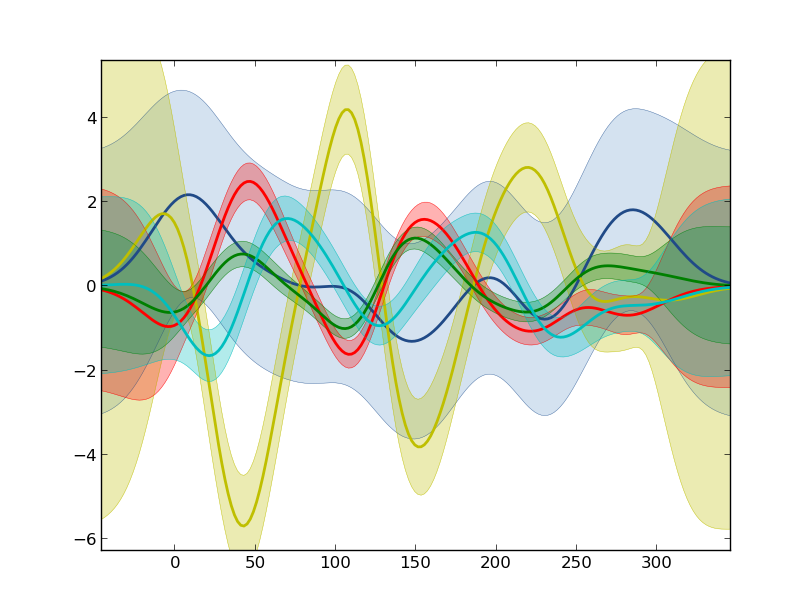
\includegraphics[width=14cm,keepaspectratio]{diagrams/RBFWh9TF.png}
		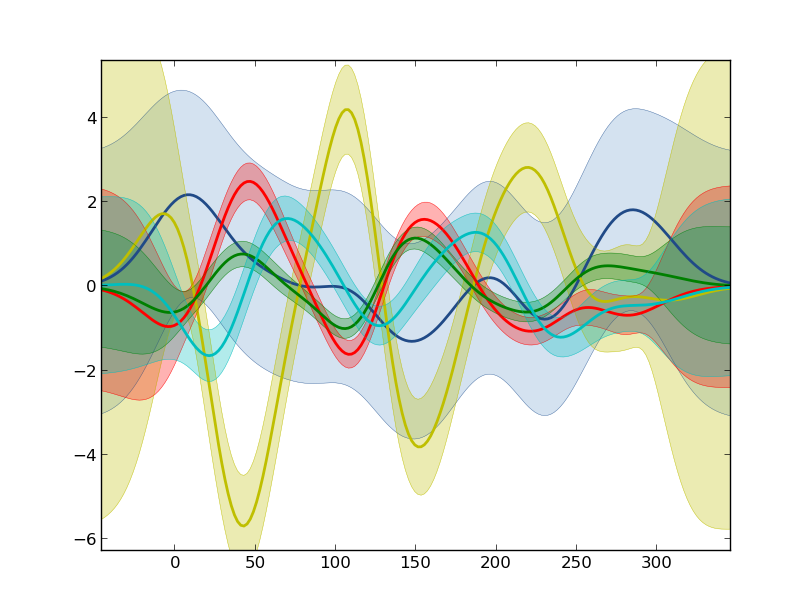
\includegraphics[width=0.9\textwidth,keepaspectratio]{diagrams/RBFWh9TF.png}
		\rule{35em}{0.5pt}
	\caption[Variation of activities of Transcription factors with RBF+white kernels]
		{Variation of activities of Transcription factors RBF+white kernels}
	\label{fig:TFA_with_RBFnWhKernel}
\end{figure}

\begin{figure}[]
	\centering
		%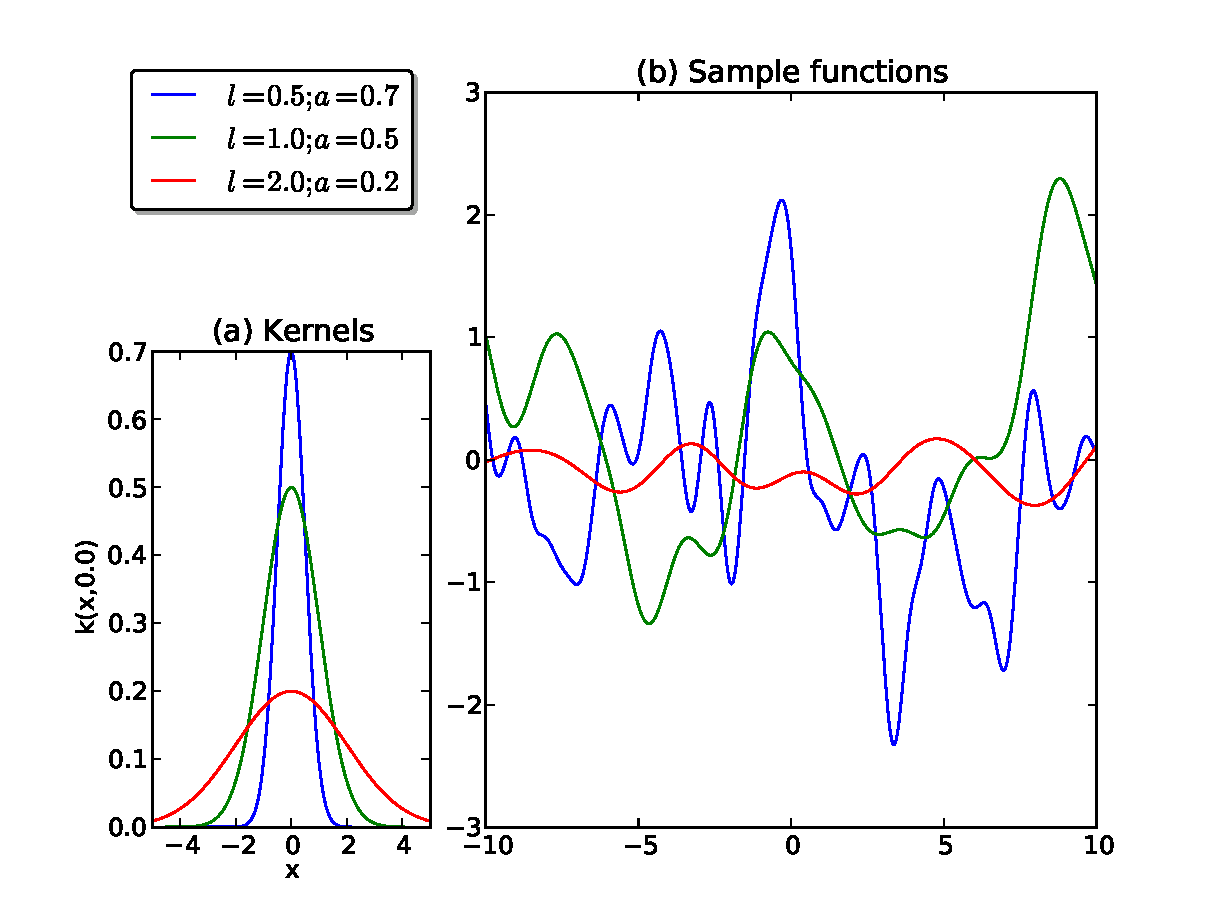
\includegraphics[width=10cm,keepaspectratio]{diagrams/SE_cov.pdf}
		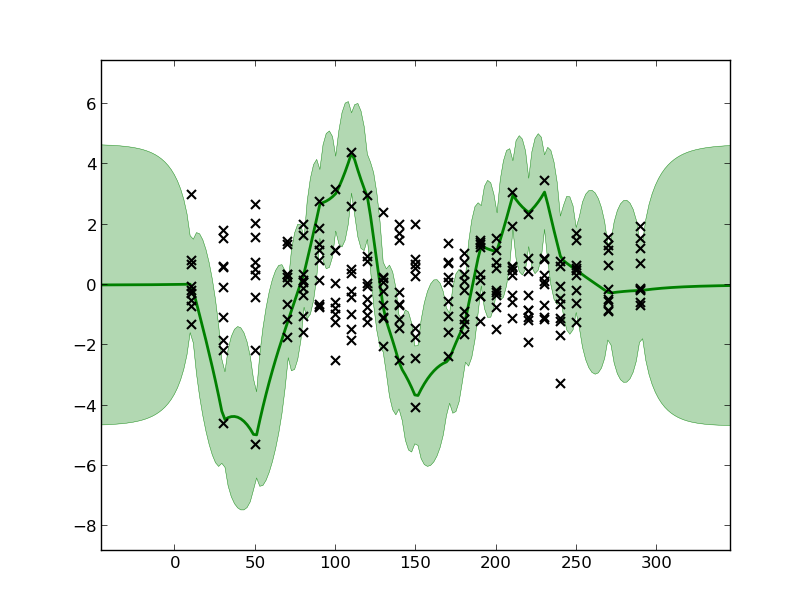
\includegraphics[width=0.9\textwidth,keepaspectratio]{diagrams/ACE2_OU_Wh_9TF.png}
		\rule{35em}{0.5pt}
	\caption[Transcription factor activity of ACE2]
		{Transcription factor activity of ACE2}
	\label{fig:TFA_of_of_ACE2}
\end{figure}
Exponentiated Quadratic kernel is very smooth kernel compared to Ornstein-Uhlenbeck kernel and 
perhaps is not a very good choice for the determination of actual transcription factors activities.
Still it can figure out the basic nature of the activities with over smoothness.
Figure \ref{fig:TFA_with_RBFnWhKernel} shows activities of different transcription factors while
the model was developed considering Exponentiated Quadratic kernel with White kernel in additive form.

Figure \ref{fig:TFA_of_of_ACE2}\footnote{The complete model is still in progress. 
After the final model exact figure might be updated from this one}
shows transcription factor activity of ACE2.
While developing the model we choose Ornstein-Uhlenbeck kernel and White kernel in additive form.
We believe that the Ornstein-Uhlenbeck kernel will consider the basic nature of the transcription
factors activity while White kernel will deal the noise associated the collected gene expression
data.

Figure \ref{fig:kern_6TF} shows the pictorial representation of intrinsic coregionalization kernel 
(Equation \ref{eq:K}) $\textbf{K}_f$ considering 20 transcription factors 
where covariance matrix $\boldsymbol{\Sigma}$ of  was 
constructed using Ornstein-Uhlenbeck kernel and White kernel in additive form.

\begin{figure}[t]
	\centering
		%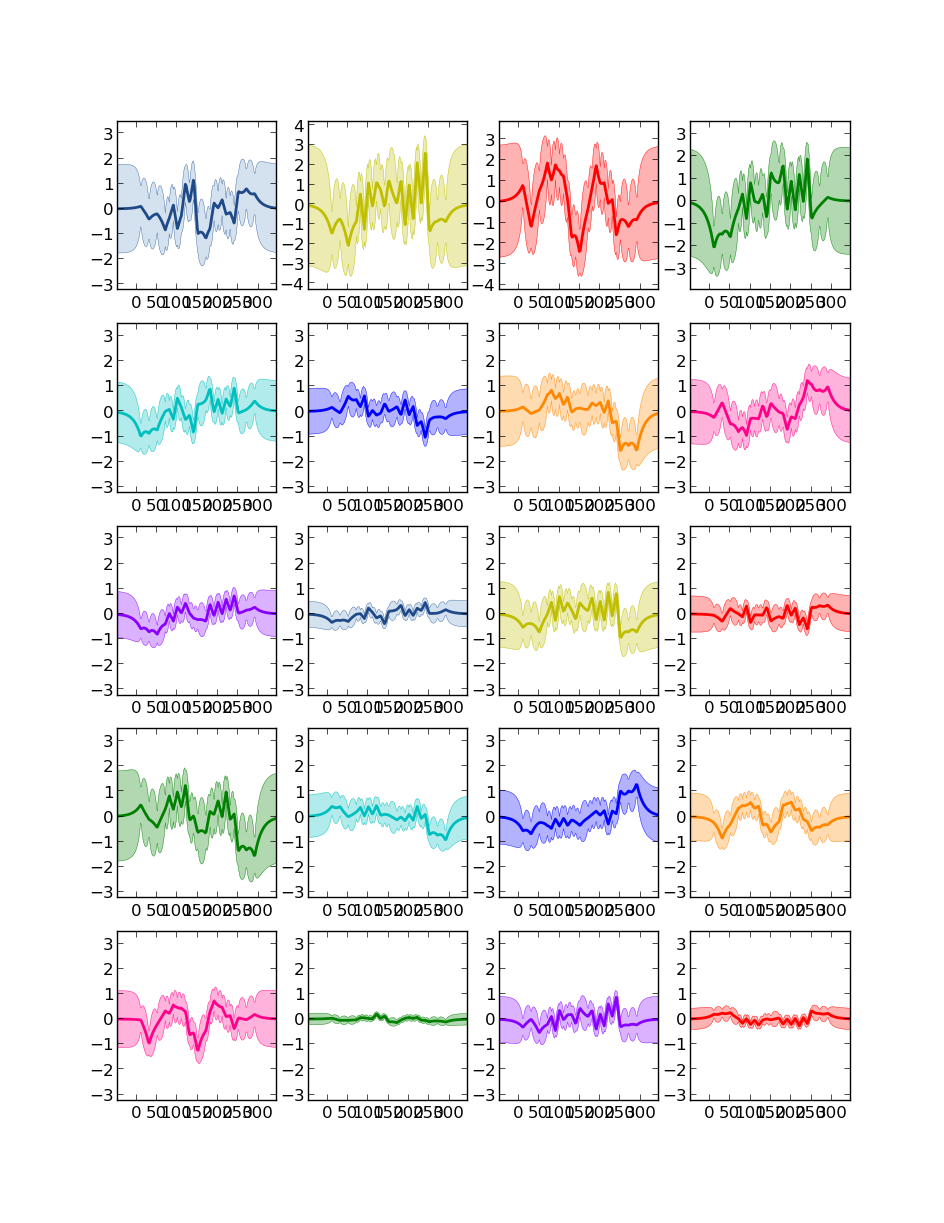
\includegraphics[width=17cm,keepaspectratio]{diagrams/OU20TF.png}
		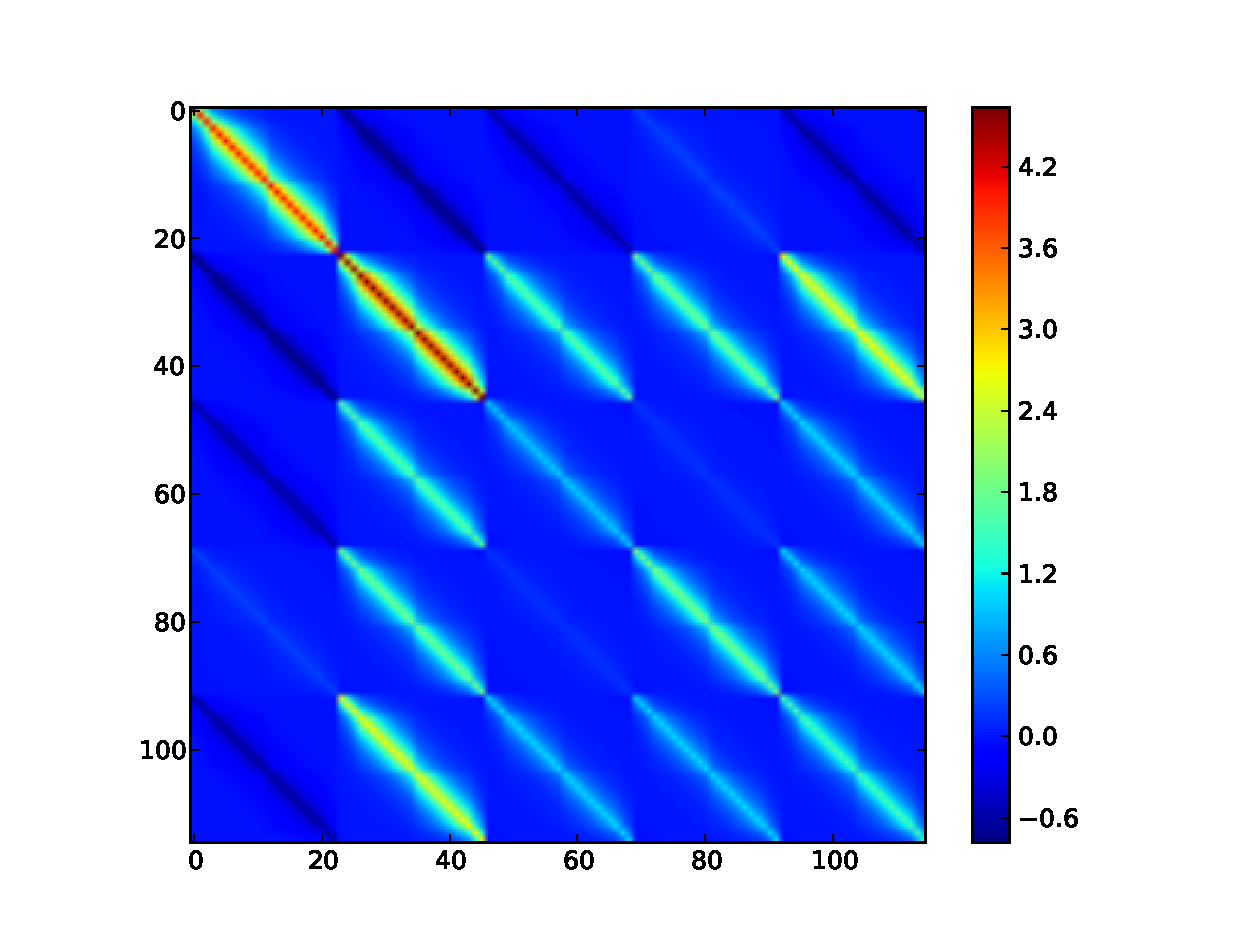
\includegraphics[width=\textwidth,keepaspectratio]{diagrams/kern_6TF.eps}
		\rule{35em}{0.5pt}
	\caption[Kernel of Intrinsic Coregionalization model $\textbf{K}_f$ considering 6 
		 Transcription factors where covariance matrix $\boldsymbol{\Sigma}$
		 was constructed using Ornstein-Uhlenbeck kernel and White kernel in additive form]
		{Kernel of Intrinsic Coregionalization model $\textbf{K}_f$ considering 6 
		 Transcription factors where covariance matrix $\boldsymbol{\Sigma}$ 
		 of $\left( Equation \ref{eq:K} \right)$ was constructed 
		 using Ornstein-Uhlenbeck kernel and White kernel in additive form}
	\label{fig:kern_6TF}
\end{figure}


Figure \ref{fig:TFA_of_20TF} shows some examples of transcription factors activities where
 model was developed with Ornstein-Uhlenbeck kernel and White kernel.

\begin{figure}[]
	\centering
		%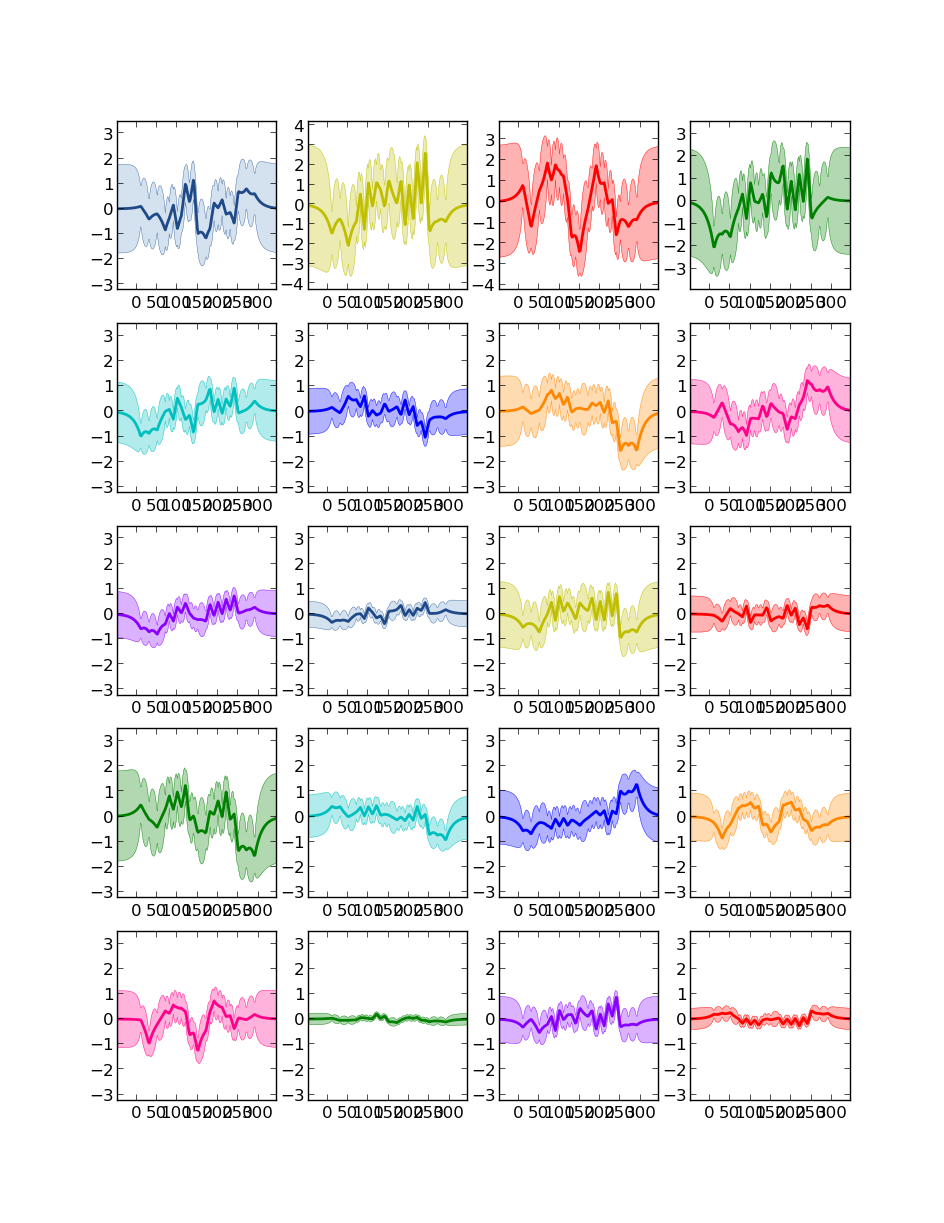
\includegraphics[width=17cm,keepaspectratio]{diagrams/OU20TF.png}
		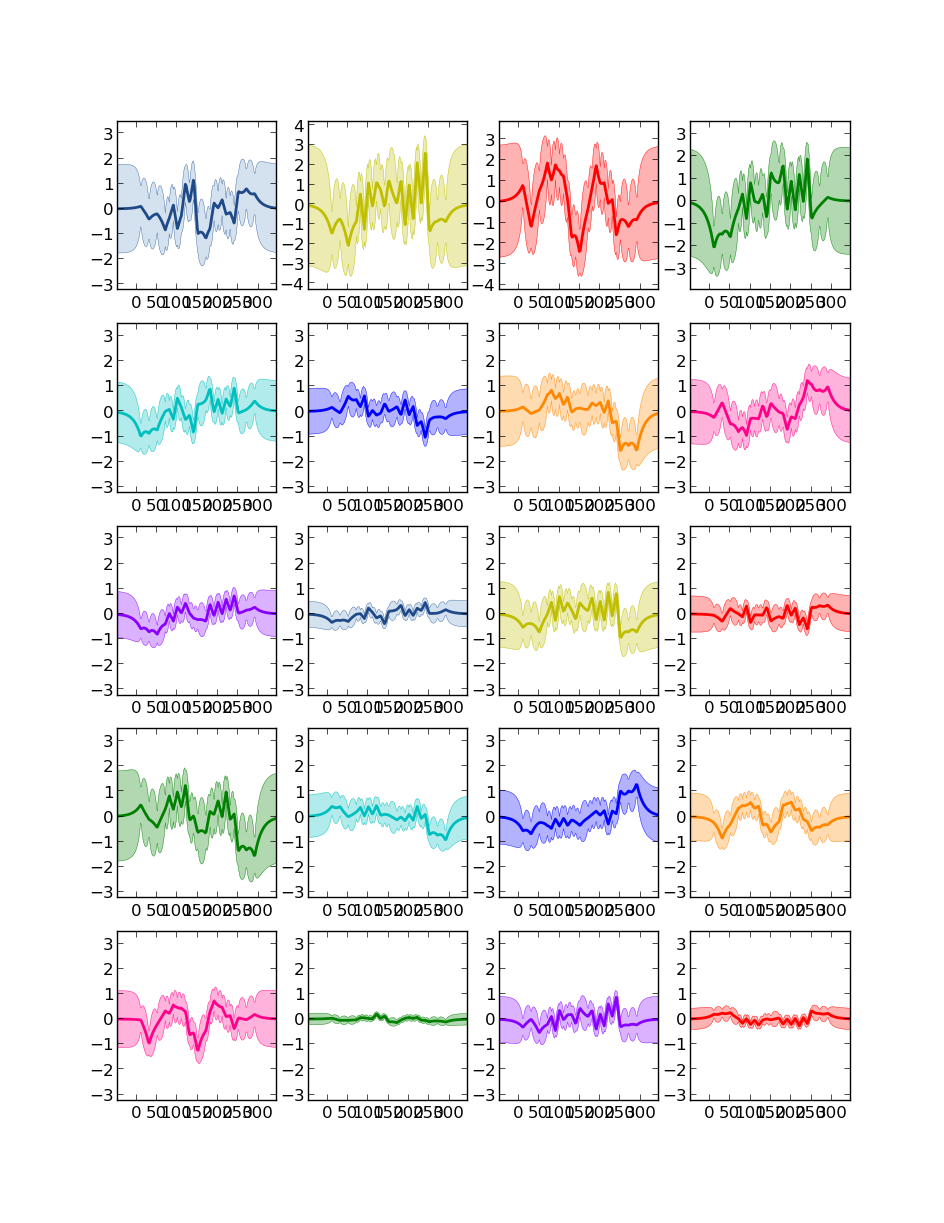
\includegraphics[width=1.1\textwidth,keepaspectratio]{diagrams/OU20TF.png}
		\rule{35em}{0.5pt}
	\caption[Transcription factor activity of different TF using Ornstein-Uhlenbeck kernel and White kernel]
		{Transcription factor activity of different TF using Ornstein-Uhlenbeck kernel and 
		White kernel in additive form}
	\label{fig:TFA_of_20TF}
\end{figure}

%TODO

\section{Making prediction}
Using Kronecker product we can rewrite the Equation \ref{eq:mGPd} as:
\begin{equation} \label{eq:predicYq}
  \mathbf{y_q}  \sim \mathcal{N} \left( \mathbf{0}, 
    \mathbf{K}_{t,t} \otimes \boldsymbol{\Lambda} \mathbf{V}^T\boldsymbol{\Sigma} \mathbf{V} \boldsymbol{\Lambda} +
    \sigma^2\mathbf{I}\right)
\end{equation}
Standard properties of multivariate Gaussian distributions tells us can split equation \ref{eq:predicYq} into
\begin{equation} \label{eq:gEp}
  \mathbf{y_q} = \mathbf{g} + \boldsymbol{\epsilon}
\end{equation}
where $\mathbf{g}$ and $\boldsymbol{\epsilon}$ are also Gaussian distributions and can be represented by:
\begin{equation}\label{eq:g}
  \mathbf{g} \sim \mathcal{N} \left( \mathbf{0}, 
    \mathbf{K}_{t,t} \otimes 
    \boldsymbol{\Lambda} \mathbf{V}^T\boldsymbol{\Sigma} \mathbf{V} \boldsymbol{\Lambda} \right)
\end{equation}
\begin{equation}\label{eq:Epsi}
  \boldsymbol{\epsilon} \sim \mathcal{N} \left(\mathbf{0},\sigma^2\mathbf{I}\right)
\end{equation}
Now we can represent the matrix $\mathbf{F}$ of transcription factor activity as:
\begin{equation}\label{eq:F}
  \mathbf{F} = \mathbf{I} \otimes \mathbf{V} \Lambda^{-1} \mathbf{g}
\end{equation}
\begin{equation}\label{eq:Sigma}
  \boldsymbol{\Sigma} = \mathbf{W}\mathbf{W}^T + diag\left(\boldsymbol{\kappa}\right)
\end{equation}
where $\boldsymbol{\kappa}$ is the kappa value from coregionalization matrix.
\begin{equation} \label{eq:predictionF}
  \mathbf{F}  \sim \mathcal{N} \left( \mathbf{0},\mathbf{K}_{t,t} \otimes \boldsymbol{\Sigma}\right)
\end{equation}
Now we can find the conditional distribution of $g$ for given $y_q$ by:
\begin{equation}\label{eq:gGivenYq}
 p\left(\mathbf{g} \middle| \mathbf{y}_q\right) \sim 
    \mathcal{N} \left( \boldsymbol{\mu}_g, \mathbf{C}_g\right)
\end{equation}
with a mean given by:
\begin{equation} \label{eq:prediction_MuG}
  \boldsymbol{\mu}_g = 
    \left[ \mathbf{K}_{t_\star,t} \otimes \boldsymbol{\Lambda} \mathbf{V}^T\boldsymbol{\Sigma} \mathbf{V} \boldsymbol{\Lambda}  \right] 
    \left[ \mathbf{K}_{t,t} \otimes \boldsymbol{\Lambda} \mathbf{V}^T\boldsymbol{\Sigma} \mathbf{V} \boldsymbol{\Lambda} + \sigma^2 \mathbf{I} \right]^{-1}\mathbf{y}_q
\end{equation}
and the covariance given by:
\begin{equation} \label{eq:prediction_Cg}
\boldsymbol{C}_g = 
    \left[ \mathbf{K}_{t_\star,t_\star} \otimes \boldsymbol{\Lambda} \mathbf{V}^T\boldsymbol{\Sigma} \mathbf{V} \boldsymbol{\Lambda}  \right] - \\
    \left[ \mathbf{K}_{t_\star,t} \otimes \boldsymbol{\Lambda} \mathbf{V}^T\boldsymbol{\Sigma} \mathbf{V} \boldsymbol{\Lambda}  
    \left[ \mathbf{K}_{t,t} \otimes \boldsymbol{\Lambda} \mathbf{V}^T\boldsymbol{\Sigma} \mathbf{V} \boldsymbol{\Lambda} + \sigma^2 \mathbf{I} \right]^{-1} 
    \mathbf{K}_{t_\star,t} \otimes \boldsymbol{\Lambda} \mathbf{V}^T\boldsymbol{\Sigma} \mathbf{V} \boldsymbol{\Lambda} \right]
\end{equation}

The mean of the conditional distribution of Equation \ref{eq:predicYq} %\ref{eq:predictionTFA} 
is:
\begin{equation} \label{eq:prediction_MuF}
  \boldsymbol{\mu}_F = 
    \mathbf{K}_{t_\star,t} \otimes \boldsymbol{\Sigma} \mathbf{V} \boldsymbol{\Lambda}
    \left[ \mathbf{K}_{t,t} \otimes \boldsymbol{\Lambda} \mathbf{V}^T\boldsymbol{\Sigma} \mathbf{V} \boldsymbol{\Lambda} + \sigma^2 \mathbf{I} \right]^{-1}\mathbf{y}_q
\end{equation}

and the covariance of the conditional distribution of Equation \ref{eq:predicYq} %\ref{eq:predictionTFA} 
given by:
\begin{equation} \label{eq:prediction_CF}
  \boldsymbol{C}_F = 
    \mathbf{K}_{t_\star,t_\star} \otimes \boldsymbol{\Sigma} -
    \mathbf{K}_{t_\star,t} \otimes \boldsymbol{\Sigma}\mathbf{V} \boldsymbol{\Lambda}
    \left[ \mathbf{K}_{t,t} \otimes \boldsymbol{\Lambda} \mathbf{V}^T\boldsymbol{\Sigma} \mathbf{V} \boldsymbol{\Lambda} + \sigma^2 \mathbf{I} \right]^{-1} 
    \left[ \mathbf{K}_{t_\star,t} \otimes \boldsymbol{\Lambda} \mathbf{V}^T\boldsymbol{\Sigma}\right]
\end{equation}

 
% Chapter 5

\chapter{Conclusion and Future work} % Main chapter title

\label{Chapter6} % For referencing the chapter elsewhere, use \ref{Chapter1} 

\lhead{Chapter 6. \emph{Conclusion and Future work}} % This is for the header on each page - perhaps a shortened title

%----------------------------------------------------------------------------------------
We have developed a tool based on programming language \emph{R} named \emph{chipDyno} using the model of
\cite{Sanguinetti:2006} which integrate the connectivity information between genes and transcription
factors, and micro array data. The probabilistic nature of the model can determine the significant
regulations in a given experimental condition.

Earlier the model was developed for a unicellular microorganism (yeast) but we have successfully
manage to determine the gene specific transcription factor activity for \textit{C. elegans}, a
multicellular eukaryote. We were also successful to filter out the quiet genes from the
differentially expressed genes.

To elucidate pathways and processes relevant to human biology 
and disease \textit{C. elegans} is been using as a vital model. 
Different orthology-prediction methods (\cite{Daniel:2011}) are using 
to compile a list of \textit{C. elegans} orthologs of human genes. Already 
a  list of 7,663 unique protein-coding genes were resulted in that list and this
represents ~38\% of the 20,250 protein-coding genes predicted in \textit{C. elegans}. 
When human genes introduced into \textit{C.Elegans} human genes replaced their homologous. 
On the contrary, many \textit{C. elegans}
genes can function with great deal of similarity to human like mammalian genes. So, 
the biological insight acquire from \textit{C. elegans} may be directly applicable to more 
complex organism like human.

Lots of computational approaches on gene expression data for time series analysis are not
well suited where time points are irregularly spaced. Even in commonly used state-space
model time points must occur at regular intervals. On the other side gene expression
experiments with regular samples may not be cost effective or optimal from the perspective of
statistics. It is expected that models with irregular time points might be more informative if 
the time points are selected considering some temporal features. Gaussian process is not 
restricted to equally spaced time series data. Already Gaussian process regression have been 
successfully applied to overcome this issue and analyse time series data (\cite{Kalaitzis:2011}).
So our expected model will overcome the restriction of temporal sampling of equally spaced
time intervals. 
%----------------------------------------------------------------------------------------

\section{Future Work}
\cite{Sanguinetti:2006} model to infer the transcription factor 
activity is a linear- Gaussian state-space model. We believe that this linear Gaussian
model is equivalent to Gaussian process with a specific covariance function.
We have developed a model directly from Gaussian process to achieve the same goal.
We are quite close to develop a valid covariance function for reconstructing transcription
factor activities given gene expression profile and binding information between genes and
transcription factors. Here we will introduce a computational trick using
singular value decomposition and intrinsic coregionalization model. We believe
this method will enable us to efficiently fit the Gaussian process in a
reduced transcription factor activity space.

Amyotrophic lateral sclerosis (ALS), also known as ``Lou Gehrig's Disease'' or motor neurone disease 
(MND), is an irreversible progressive neurodegenerative adult onset that affects motor neurons 
in the brain and the spinal cord. Muscle denervation spreads over neuromuscular system and 
leads toward death by failure of the respiratory system with in few years of system 
onset (\cite{Peviani:2010}). 
This lethal invariable disorder has median survival of less than 5 years, only 20\% 
of the affected people can survive more than 5 years and 10\% of the patients 
can survive more than 10 years. Mutation in the Cu/Zn superoxide dismutase (SOD1) gene 
is responsible for around 20\% of the familial motor neurone disease \cite{Nardo:2013}. 
Transgenic mice can express human SOD1 mutation and nicely replicates different 
histopathological and clinical features of motor neurone disease. Mimic of these murine models 
of different clinical phenotypes observed from human MND patients are widely using by the 
researchers to determine the disease progression. But we didn't found any evidence of gene expression 
analysis that attempt to analyse motor neuron disease considering the genetic background on 
different phenotype of this murine disease. So gene expression analysis for different murine models 
could reveal interesting information. 
\cite{Nardo:2013} used two mouse models to analyse fast and slow disease progression of ALS.
We will use our Gaussian process based model to infer the 
transcription factor activity on gene expression data obtained from different murine models and 
try to find out some fascinating insights.

Clustering of gene expression time series is another major interest of the research to get the view of
groups of co-regulated or associated genes. It is assumed that gene involved in the same biological 
process will be expressed with a similarity sharing underlying time series. \cite{Cossins:2007}
did some additional cluster analysis (not published yet!) based on some phenotype properties. Again 
it is very common to have multiple biological replicates of the gene expression time series data. 
Just taking average of the replicates surely lead toward discarding insight. Recently \cite{Hensman:2013} used
a hierarchy of Gaussian process to model a gene specific and replicate specific temporal covariance.
They also used this model for clustering application. Using this Gaussian process based hierarchical
clustering analysis of \cite{Hensman:2013} we will try to find some robust clusters for the gene
expression data of \textit{C. elegans}. Once if we can do so, it will easily lead us to find out the active
transcription factors related with these clusters and their subsequent dynamic behaviour as well. 
%% Chapter 7

\chapter{Intro...} % Main chapter title

\label{Chapter7} % For referencing the chapter elsewhere, use \ref{Chapter1} 

\lhead{Chapter 7. \emph{Intro...}} % This is for the header on each page - perhaps a shortened title

%----------------------------------------------------------------------------------------

For this we used the fact that $v_{k,\ell}$ is only present in the $k$ them of the sum over $i$, the other terms are zero. We then differentiate the quadratic (giving a factor of 2) and finally multiply by the gradient of $-\mathbf{u}_{i}^\top\mathbf{v}_j$ with respect to $v_{k,\ell}$ which is $-u_{i,\ell}$. 
%\input{Chapters/Chapter8} 

%----------------------------------------------------------------------------------------
%	THESIS CONTENT - APPENDICES
%----------------------------------------------------------------------------------------

\addtocontents{toc}{\vspace{2em}} % Add a gap in the Contents, for aesthetics

\appendix % Cue to tell LaTeX that the following 'chapters' are Appendices

% Include the appendices of the thesis as separate files from the Appendices folder
% Uncomment the lines as you write the Appendices

% Appendix A

\chapter{Summery of DDP Progress} % Main appendix title

\label{AppendixB} % For referencing this appendix elsewhere, use \ref{AppendixA}

\lhead{Appendix A. \emph{Summery of DDP Progress}} % This is for the header on each page - perhaps a shortened title

Based on the plan of the Doctoral Development Programme (DDP) various activities have been completed-

\section{Posters Presentation and talks}
\subsection{Posters}
\begin{itemize}
 \item Rahman M A,  Lawrence N D, ``A Probabilistic Dynamic Model for Transcription Factor Activity of C. Elegans'', Machine Learning Summer School and AISTATS joint poster session, Reykjavic, Iceland 2014.
\end{itemize}
\subsection{Workshop Notebook}
\begin{itemize}
 \item Rahman M A,  Lawrence N D, ``Inferring Transcription Factor Activities by Combining Binding Information with Gene Expression Profiles'', Available online, url-
 \url{http://nbviewer.ipython.org/github/SheffieldML/notebook/blob/master/compbio/transcriptionFactorActivities.ipynb}
\end{itemize}
\subsection{Talks}
\begin{itemize}
 \item Rahman M A, Lawrence N D, ``Dynamic model for transcription factor activity of C. Elegans'', Sheffield Institute for Translational Neuroscience (SITraN), University of Sheffield, November 2013.
 \item Rahman M A, Lawrence N D, ''A probabilistic dynamic model for transcription factor activity of C. Elegans``, Sheffield Institute for Translational Neuroscience (SITraN), University of Sheffield, May 2013.
\end{itemize}


\section{Participation in Conference, Workshop and Summer schools}

As a part of DDP progress I have participated a number of Conference, Workshop and Summer schools given bellow-
\begin{itemize}
\item Gaussian Process Summer School 2013, University of Sheffield, UK was organized by our lab ML@SITraN from June 10 to June 12, 2013 followed by Workshop on Latent Force Model 2013. I was an organizing member here.
\item I have attended the Natural Computing Applications Forum (NCAF) Meeting at University of Oxford, Oxford, UK from July 04 to July 05, 2013.
\item I have attend the Machine Learning Summer School (Advanced Topics in Machine Learning) at Technical University of Denmark, Copenhagen, Denmark on August 2013.
\item Gaussian Process Winter School 2014, University of Sheffield, UK was organized by our lab ML@SITraN from January 13 to January 16, 2014. I was a organizing member here. Workshop on Spatiotemporal Modelling with Gaussian Processes was collocated with GPWS 2014.
\item I have attended the Mathematical and Statistical Aspects of Molecular Biology (MASAMB) 2014 workshop at University of Sheffield, UK from April 09 to April 10, 2014
\item I have attended the conference of Artificial Intelligence and Statistics (AISTATS) 2014 at Reykjavik, Iceland followed by the Machine Learning Summer School (MLSS2014).
\item Gaussian Process Summer School 2014, University of Sheffield, UK was organized by our lab ML@SITraN from September 15 to September 17, 2014. Workshop on Gaussian Processes for Feature Extraction was collocated with GPSS 2014. I was a organizing member here.
\end{itemize}

\section{Demonstration}
As a part of DDP progress the activities relating to teaching and demonstrating are given bellow-
\begin{itemize}
\item COM4509/COM6509 Machine Learning and Adaptive Intelligence with Professor Neil D Lawrence(ACADEMIC YEAR 2014-15). 
\item COM161: Introduction to Programming and Problem-Solving and COM160: Computer Problem Solving and Object-Oriented Design with Professor Mark Hepple (ACADEMIC YEAR 2014-15).
\item COM1005/COM2007: Machines and Intelligence with Professor Rob Gaizauskas (ACADEMIC YEAR 2014-15).
\item FCE101: Introduction to Bioengineering (ACADEMIC YEAR 2011-12) with Professor Neil D lawrence.
\end{itemize}

\section{Participation in DDP Courses}
To improve the core concepts of research I have attended the following courses/modules:

\begin{itemize}
 \item COM - COM4509~COM6509: Machine Learning and Adaptive Intelligence(GRADUATE YEAR 2011-12).
 \item COM4508/6508: Introduction to Computational Systems Biology (GRADUATE YEAR 2011-12).
 \item FCE - FCE6100: Research Ethics and Integrity (GRADUATE YEAR 2011-12).
 \item COM - COM6930: Research Teamwork in Computer Science (GRADUATE YEAR 2011-12).
 \item COM - COM6940: Presentation of Computer Science Research (GRADUATE YEAR 2011-12).
 \item COM - COM6950: Developments in Computer Science (GRADUATE YEAR 2011-12).
\end{itemize}

\section{Other activities related to DDP}
\begin{itemize}
 \item Take part in the poster presentation at the research retreat of Department of Computer Science, University of Sheffield.
 \item Reading, understanding and writing about relevant research, and implementing simple algorithms to improved research related skills.
 \item Maintaining a personal website detailing any research and experiments that have been done.
 \item Made contact with experts from a different department/universities to get the in-depth knowledge on Machine Learning and System Biology.
\end{itemize}
%\input{Appendices/AppendixB}
%\input{Appendices/AppendixC}

\addtocontents{toc}{\vspace{2em}} % Add a gap in the Contents, for aesthetics

\backmatter

%----------------------------------------------------------------------------------------
%	BIBLIOGRAPHY
%----------------------------------------------------------------------------------------

\label{Bibliography}

\lhead{\emph{Bibliography}} % Change the page header to say "Bibliography"

%\bibliographystyle{unsrtnat} % Use the "unsrtnat" BibTeX style for formatting the Bibliography

%\bibliography{Bibliography} % The references (bibliography) information are stored in the file named "Bibliography.bib"

\bibliographystyle{apalike}
%\bibliographystyle{plainnat}

\bibliography{Bibliography}

%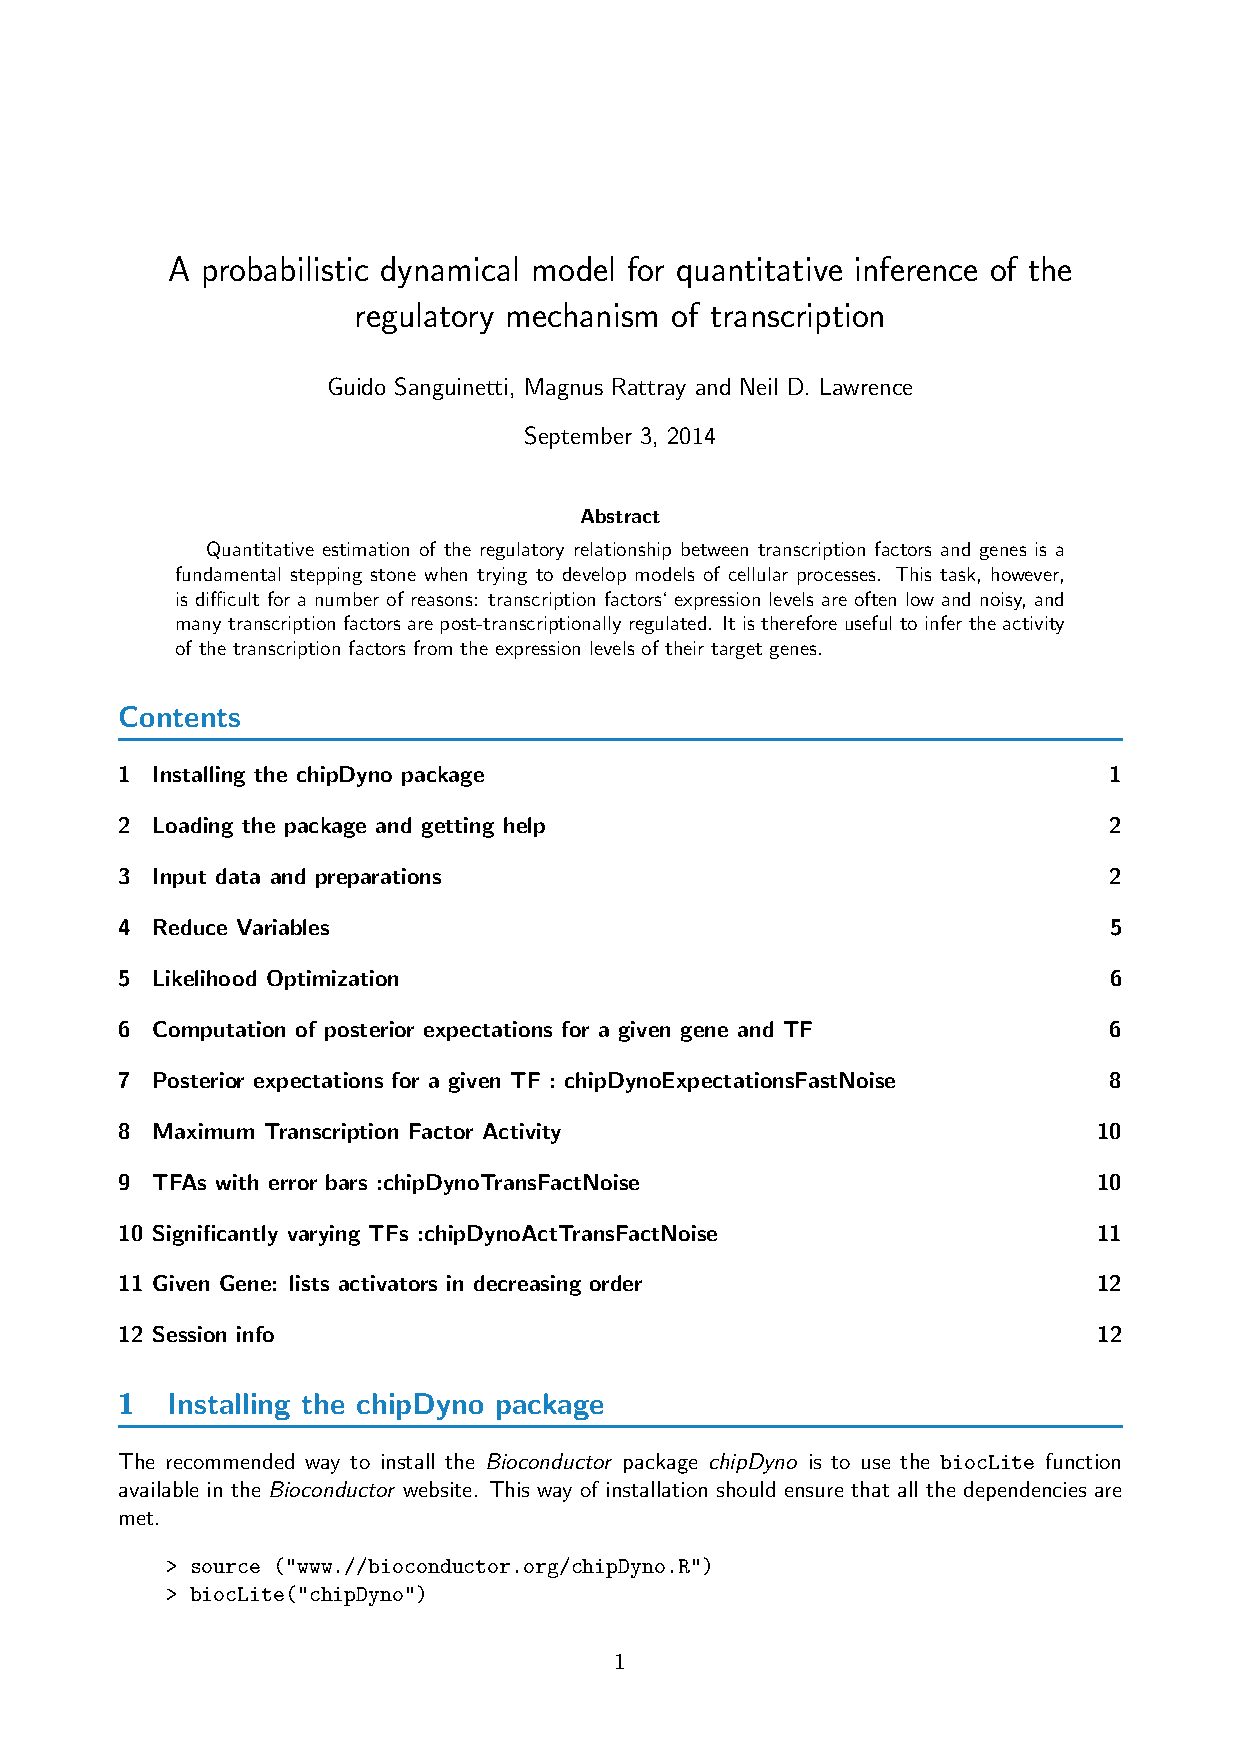
\includepdf[pages=-]{/home/muhammad/Dropbox/Git/mlprojects/chipDyno/SweaveDoc/chipDyno_test.pdf}
% pdftk main.pdf chipDyno_test.pdf cat output report.pdf

%pdftk main.pdf chipDynoForReport.pdf cat output muhammadTransferReportDraft.pdf
%pdftk main.pdf GanttchartTransferReport.pdf chipDynoForReport.pdf cat output muhammadTransferReport.pdf


\end{document}  

%pdflatex -shell-escape main.tex
%pdftotext main.pdf - | egrep -e '\w\w\w+' | iconv -f ISO-8859-15 -t UTF-8 | wc -w